\documentclass[12pt]{amsart}

\usepackage{amssymb,amsfonts,amsmath,amsthm}
\usepackage[dvipsnames]{xcolor}
\usepackage{enumerate,enumitem,tikz-cd,tikz,mathrsfs,graphicx,marvosym,wasysym,epigraph,afterpage}
%mathrsfs is for \mathscr, marvosym for \Coffeecup, graphicx for \heartsuit, wasysym is for \twonotes
\usepackage[colorlinks=true, urlcolor=purple, linkcolor=RoyalBlue, citecolor=magenta, pdfborder={0 0 0}]{hyperref}
%\usepackage[document]{ragged2e}
\usetikzlibrary{backgrounds}

\setlength\epigraphwidth{.6\textwidth}
%\setlength\epigraphrule{0pt}
\setlength{\parindent}{0pt}

\newcommand\blankpage{
    \null
    \thispagestyle{empty}
    \addtocounter{page}{-1}
    \newpage}

\newtheorem{thm}{Theorem}[section]
\newtheorem{cor}[thm]{Corollary}
\newtheorem{prop}[thm]{Proposition}
\newtheorem{lem}[thm]{Lemma}
\newtheorem{defn}[thm]{Definition}
\theoremstyle{definition} 
\newtheorem{exmp}[thm]{Example}
\newtheorem{rem}[thm]{Remark}


\begin{document}
\begin{titlepage}
  \begin{center}
\begin{tikzpicture}
\node[opacity=0.7] at (0,0) {
\includegraphics[width=4cm]{LOGO}};  
\end{tikzpicture}
  \end{center}
\begin{center}
{\small{ FACOLT\`A DI SCIENZE MATEMATICHE FISICHE E NATURALI\\
Corso di Laurea Magistrale in Matematica}}
\end{center}
\vspace{20 mm}

\begin{center}
{\huge \texttt{FUNCTORIAL FLAVOURS}}  \\
\vspace{5 mm}
{\huge \texttt{OF BRIDGELAND'S SLICINGS}}
\vspace{40mm}
\end{center}
\par
\noindent
\begin{minipage}[t]{0.49\textwidth}
{\large{ Advisor:\\
Prof.\\
Domenico Fiorenza}
\begin{center}
\begin{tikzpicture}
\node at (0,0) {
\includegraphics[width=5cm]{firmaprof}};  
\end{tikzpicture}
\end{center}
}
\end{minipage}
\hfill
\begin{minipage}[t]{0.49\textwidth}\raggedleft
{\large{ Candidate:\\
Giovanni Luca Marchetti\\
serial 1574632}
\begin{center}
\begin{tikzpicture}
\node at (0,0) {
\includegraphics[width=5cm]{firmamia}};  
\end{tikzpicture}
\end{center}
}
\end{minipage}
\vspace{18mm}
\begin{center}
{\large{ Sessione Estiva \\Anno Accademico 2016-2017}\\
Dipartimento di Matematica `Guido Castelnuovo'}
\end{center}
\end{titlepage}

\clearpage
\afterpage{\blankpage}

\clearpage
\epigraph{\textit{I should have been a pair of ragged claws \\ Scuttling across the floors of silent seas.}}{T. S. Eliot}
\vspace{40 mm}

\begin{tikzpicture}[overlay]
\node[opacity=0.1] at (6.3,-1) {
\includegraphics[width=30cm]{Libra}};  
\end{tikzpicture}
{
\hypersetup{linkcolor=black} 
\tableofcontents 
}

\newpage
\thispagestyle{empty}
\vspace*{50 mm}
\begin{flushright}
\textit{\`{A} la folie.}
\end{flushright}
\section{Ouverture}
\epigraph{\textit{Professor Soergel studies the fact that the sphere is round, and he likes it.}}{???}
\vspace{10 mm}
One manifestly challenging and highly creative task is to capture the geometry of some space (whatever the latter means) via clear and clean information. An historically notable breakthrough in that direction is probably the discovery by Euler of his famous formula for convex polyhedra, which we can regard as the date of birth of homological algebra. It was clear since then that a space should be regarded as a numerical (or, more generally, algebraic) object sliced into pieces, each describing the features appearing at a given dimensional level. These pieces interact by means of a 'boundary' map forming what we call today a 'chain complex' (i.e., an objects of a derived category), whose '(co)homology' measures how distant is the geometry from being quite trivial (having no holes, for example). However, there is also another interaction appearing when considering what's happening above a fixed dimension and not exactly in it; one obtains different maps arranged in a sequence called 'Postnikov tower', in honour of the well known parallel behavior arising in topology. The scope of this thesis is indeed to convince the reader that these towers synthesize most of the foundational aspects of homological algebra and allow us to understand fractal noninteger dimensions by slicing (algebrisations of) spaces into finer pieces. \\

We shall now get more in detail. As mentioned above, by (co)homology we mean the well known functor $$\mathscr{D}^b(\mathscr{A}) \overset{H^n}{\longrightarrow} \mathscr{A}$$ from the (bounded) derived category of some abelian category $\mathscr{A}$ to $\mathscr{A}$ itself. We shall expand our classical view of cohomology by first regarding these data from a different perspective. Truncating a complex in $\mathscr{D}^b(\mathscr{A})$ at the indices in which its cohomology doesn't vanish defines a factorization of the initial morphism, the abovementioned Postnikov tower of the complex, whose successive cones are, up to translation, the cohomology of the complex (with decreasing indices) and thus lie in $\mathscr{A}[n]$ for some $n \in \mathbb{Z}$ (where we think of $\mathscr{A}$ sitting in its derived category as the complexes concentrated in degree $0$). We then have a collection $\{ \mathscr{A}[n] \}_{n \in \mathbb{Z}}$ of subcategories indexed by integers which induces Postikov towers. This, with the obvious vanishing property of negative Ext groups, is the celebrated concept of 'bounded t-structure' ('t' stands for 'truncation') by Beilinson, Bernstein and Deligne. We can now think of a bounded t-structure (which makes sense in abstract triangulated categories) as a generalized cohomology theory: indeed, the abelianity of the subcategories we consider (which are the same up to translation) and the functoriality of the cones of the Postnikov towers (which we think of as the cohomology induced by the bounded t-structure) are automatic. A triangulated category tipically contains a lot of bounded t-structures different from the 'standard' one we described above, the most famous (and firstly discovered) being the one of 'perverse sheaves' on a stratified space. \\

By going deeper, a crucial motivation can be found in the ideas of David Mumford. We consider a compact Riemann surface $C$. For a coherent sheaf $F$ we can define its phase as $$- \frac{\textnormal{rk}(F)}{\textnormal{deg}(F)} \in \overline{\mathbb{Q}}=\mathbb{Q} \sqcup \{ \infty \}$$ 
We call a sheaf semistable if all its subsheaves have smaller phase and denote $\mathscr{P}_{\phi}$ the full subcategory of semistable sheaves of phase $\phi$. Now we again have a collection $\{ \mathscr{P}_{\phi} \}_{\phi \in \overline{\mathbb{Q}}}$ of subcategories of $\textnormal{Coh}(C)$ with a similar vanishing property (there is no nonzero morphism between two semistable sheaves if the first one has strictly greater phase). Moreover, each coherent sheaf has a filtration by subobjects, called 'Harder-Narasimhan filtration', whose successive quotients are semistable with decreasing phase. Combining these filtrations with the Postnikov towers of the standard t-structure on $\mathscr{D}^b(\textnormal{Coh}(C))$, one gets a collection $$\{ \mathscr{P}_{\phi}[n] \}_{(n,\phi) \in \mathbb{Z} \times \overline{\mathbb{Q}}}$$ of subcategories which has its own Postnikov towers with decreasing indices with respect to the lexicographical product on $\mathbb{Z} \times \overline{\mathbb{Q}}$. Now, if we choose a monotne embedding of $\overline{\mathbb{Q}}$ into the interval $]0,1] \subseteq \mathbb{R}$, then we get an embedding $$\mathbb{Z} \times \overline{\mathbb{Q}} \hookrightarrow \mathbb{Z} \times ]0,1] = \mathbb{R}$$ 
and we can then think of our subcategories as indexed by real numbers. These kind of phenomena also appear in string theory as '$\Pi$-stability': physicists think of $D$-branes as coherent sheaves on a Calabi-Yau manifold, and systems of (anti-)$D$-branes linked by tachyons as complexes of sheaves. Then a phase of such a system is a real number (the argument of its central charge precisely) that counts its symmetries and, by defining semistable branes just as in Mumford stability, one has an approximation (or 'decay', in a more concrete language) of each object in the derived category by semistables of decreasing phase. In other words, one gets Postnikov towers again.  \\

All this motivated Tom Bridgeland to define an $\mathbb{R}$-slicing in a triangulated category as a collection of subcategories indexed by real numbers with the above properties (vanishing and existence of Postnikov towers), generalizing both bounded t-structures and Mumford stability. Those $\mathbb{R}$-slicings can finally be regarded as cohomology theories where dimension is allowed to be real (intead of just integer). Thinking of the above example from string theory, this point of view reminds of Poincare's philosophy: dimension is just a shadow of simmetry, and thus it is natural to index both cohomology and simmetries by the same set. However, from a formal perspective, Bridgeland's approach is slightly redundant: both the main definition and its basic properties don't depend on any special feature of $\mathbb{R}$, but just on its ordering and the action it carries by $\mathbb{Z}$. Following Gorodentsev, Kuleshov and Rudakov, this leads us to introduce the notion of $\mathbb{Z}$-poset and consider $J$-slicings, where $J$ is a $\mathbb{Z}$-poset, as an immediate generalization of Bridgeland's ones. In this unified language, many things appear clearer: the set of all $J$-slicings on a fixed triangulated category is functorial in $J$ and this gives rise to a very natural approach to tilting theory by Happel, Reiten and Smal\o{} and can be exploited to recover classical constructions of nonstandard bounded t-structures like perverse sheaves and the diagonal t-structure from Koszul duality in a simple way.\\ 

Moreover, the formalism of $\mathbb{R}$-slicings doesn't explain the theory of semiorthogonal decompositions: these are important objects which appear in many areas of literature (and are intesively used even in the the context of Bridgeland stability) and arise in our language as $J$-slicings when $\mathbb{Z}$ acts trivially on $J$. Such $J$'s clearly don't map to $\mathbb{R}$ as $\mathbb{Z}$-posets, and thus semiorthogonal decompositions cannot be reconducted to Bridgeland's slicings. Another reason to pursue such a generality is the fact that Mumford stability extends to higher dimensional varieties as Gieseker stability, where the phase of a sheaf becomes its whole Hilbert function. This means that in this case $J$ should be taken as a set of polynomial germs with some natural ordering, and $\mathbb{R}$ is then again not sufficient. \\

Needless to say, the language of categories will serve us as a main tool. Besides the examples, which will be taken from all around, this thesis is purely categorical. The main backround required to the reader is some knowledge of algebraic categories (abelian and their derived ones) and basics from order theory. \\ \\

%\subsection{Ringraziamenti} Per difesa o per amore

\afterpage{\blankpage}
\section{Abstract homological algebra}
\epigraph{\textit{Tea is nought but this: first you heat the water, then you make tea. Then you drink it properly. That is all you need to know.}}{Sen No Rikyu}
\vspace{10 mm}
Before starting, let us fix some anti-Bourbaki categorical conventions. We'll often consider objects of a category up to isomorphism. This means, for example, that when an isomorphism is obvious or canonical we'll just write equality and that all subcategories are assumed to be saturated (i.e. closed under isomorphisms). To keep things clean, we will avoid writing names for morphisms as much as possible and will denote $1$ the identity of any object in any category. We do not really care about foundational issues and will almost always assume our categories to be (essentially) small. There will occasionaly be lines preceeded by the \twonotes \ symbol. Those will be just vague streams of consciousness and are mainly meant as decorations. \\

\subsection{Triangulated categories}
We begin by introducing the abstract framework in which homological algebra usually takes place: the so called triangulated categories. These are immediate generalizations of derived categories which do not depend on an underlying abelian category. Indeed, one just has a notion of 'distinguished triangle', which we can think of as some kind of short exact sequence, and an autoequivalence which corresponds to shifting the indices of a complex in the derived category. By attaching a distinguished triangle to its shifts one builds up the idea of induced long exact sequence and this is the essential tool of homological algebra. \\

Triangulated categories first appeared in Jean-Louis Verdier's PhD thesis supervised by Alexander Grothendieck (\cite{ver}), still a solid reference today. A more modern and ramified treatment can be found in the classical textbook \cite{gel}. However, we give a slightly different presentation: following \cite{may}, one of the usual axioms for triangulated categories results redundant and we prove it as a proposition accordingly. On the other hand, as it had been for many years with the fifth postulate in euclidean geometry and with the axiom of choice in set theory, it is not known whether \textit{(Tr4)} below follows from the other axioms. 

\begin{defn}
Let $\mathscr{D}$ be an additive category, $\Sigma$ an additive autoequivalence of $\mathscr{D}$. We denote for all $n \in \mathbb{Z}$, $*[n]=\Sigma^n(*)$. A \textbf{triangle} in $\mathscr{D}$ is a diagram of the form $X \longrightarrow Y \longrightarrow Z \longrightarrow X[1]=\Sigma(X)$, which we denote for simplicity: $$X \longrightarrow Y \longrightarrow Z \longrightarrow$$
The triangles of $\mathscr{D}$ form then an additive category, where the morphisms are triples $a,b,c$ fitting in a commutative diagram: 
\begin{center}
\begin{tikzcd}[ampersand replacement=\&]
X \arrow{r} \arrow{d}{a} \& Y \arrow{r} \arrow{d}{b} \& Z \arrow{d}{c} \arrow{r} \& X[1] \arrow{d}{a[1]} \\
X' \arrow{r} \& Y' \arrow{r} \& Z' \arrow{r} \& X'[1]
\end{tikzcd}
\end{center}
A \textbf{triangulated category} is an additive category $\mathscr{D}$ equipped with an additive autoequivalence $\Sigma$, called \textbf{translation}, and a full (saturated) subcategory of its triangles $\bigtriangleup$, whose objects we call \textbf{distinguished triangles} of $\mathscr{D}$, so that: 
\begin{enumerate}
\item [(Tr1)] The triangle $$X \overset{1}{\longrightarrow} X \longrightarrow 0 \longrightarrow$$ is distinguished. We call it the \textbf{trivial} triangle.
\item [(Tr2)] Any morphism $X \longrightarrow Y$ in $\mathscr{D}$ extends to a distinguished triangle $X \longrightarrow Y \longrightarrow Z \longrightarrow $. We call $Z$ a \textbf{cone} of that morphism. 
\item [(Tr3)] The triangle $X \overset{f}{\longrightarrow} Y \longrightarrow Z \longrightarrow $ is distinguished if and only if the triangle $$Y \longrightarrow Z \longrightarrow  X[1]  \overset{-f[1]}{\longrightarrow} $$ is distinguished. We call the second triangle the \textbf{rotation} of the first one.
\item [(Tr4)] If  $X \overset{f}{\longrightarrow} Y \overset{h}{\longrightarrow} Z' \longrightarrow $, $Y \overset{g}{\longrightarrow} Z \longrightarrow X' \longrightarrow$ and $X \overset{gf}{\longrightarrow} Z \longrightarrow Y'$ are distinguished triangles, then there is a distinguished triangle $Z' \longrightarrow Y' \longrightarrow X' \longrightarrow $, called a \textbf{braid} generated by $gf$, so that the following commutes: \\
\begin{center}
\scalebox{0.8}{
\begin{tikzcd}[ampersand replacement=\&]
  X \arrow[bend left=35]{rr}{gf} \arrow{rd}{f} \& \&  Z \arrow[bend left=35]{rr} \arrow{rd} \& \& X' \arrow[bend left=35]{rr} \arrow{rd} \& \& Z'[1] \\
 \& Y \arrow{ru}{g} \arrow{rd}{h} \& \& Y' \arrow{ru} \arrow{rd} \& \& Y[1] \arrow{ru}{h[1]} \& \\
 \& \& Z' \arrow{ru} \arrow[bend right=35]{rr} \& \& X[1] \arrow{ru}{f[1]} \& \&
\end{tikzcd}
}
\end{center}
\end{enumerate}
\end{defn}

Let $\mathscr{D}$ be a triangulated category. Observe that the opposite category $\mathscr{D}^{\textnormal{op}}$ equipped with translation functor $\Sigma^{-1}$ is clearly triangulated.\\
We put the sign in \textit{(Tr3)} because, if $X \overset{f}{\longrightarrow} Y \overset{g}{\longrightarrow} Z \overset{h}{\longrightarrow} $ is a distinguished triangle in $\mathscr{D}$, each three consecutive morphisms in the following long sequence form a distinguished triangle: $$\cdots \overset{-g[-1]}{\longrightarrow} Z[-1] \overset{-h[-1]}{\longrightarrow} X \overset{f}{\longrightarrow} Y \overset{g}{\longrightarrow} Z \overset{h}{\longrightarrow} X[1] \overset{-f[1]}{\longrightarrow} Y[1] \overset{-g[1]}{\longrightarrow} \cdots$$ 

\begin{exmp}\label{bbe}
Let $\mathscr{A}$ be an abelian category. Recall that its derived category $\mathscr{D}(\mathscr{A})$ is the homotopy category of chain complexes in $\mathscr{A}$ localized to quasi-isomorphisms (i.e. morphisms which induce isomorphisms in homology). The translation functor of $\mathscr{D}(\mathscr{A})$ shifts the indices of a complex and changes the sign of the differential. Moreover, the cone $\textnormal{cone}(f)$ of a morphism $f$ of complexes is the total complex of $f$ (seen as a double complex). If we take as distinguished triangles in $\mathscr{D}(\mathscr{A})$ those isomorphic to triangles of the form $$X \overset{f}{\longrightarrow} Y \longrightarrow \textnormal{cone}(f) \longrightarrow$$
the derived category becomes tiangulated. Moreover, the bounded derived category $\mathscr{D}^b(\mathscr{A})$ (consisting of complexes with homology vanishing for a cofinite set of indices) is a triangulated subcategory of $\mathscr{D}(\mathscr{A})$. 
\end{exmp}

\begin{prop}\label{s}
\textnormal{($3 \times 3$ Lemma)} Suppose that $X \overset{f}{\longrightarrow} Y \overset{g}{\longrightarrow} Z \overset{h}{\longrightarrow}$, $X' \overset{f'}{\longrightarrow} Y' \longrightarrow Z' \longrightarrow $, $X \overset{a}{\longrightarrow} X' \overset{a'}{\longrightarrow} X'' \overset{a''}{\longrightarrow} $, $Y \overset{b}{\longrightarrow} Y' \longrightarrow Y'' \longrightarrow $ are distinguished triangles in $\mathscr{D}$. If the upper left square of the below diagram commutes, then there are distinguished triangles $Z \longrightarrow Z' \longrightarrow Z'' \longrightarrow $, $X'' \longrightarrow Y'' \longrightarrow Z'' \longrightarrow $ so that the following commutes:  
\begin{center}
\begin{tikzcd}[ampersand replacement=\&]
X \arrow{r}{f} \arrow{d}{a} \& Y \arrow{r}{g} \arrow{d}{b} \& Z \arrow{r}{h} \arrow{d} \& X[1] \arrow{d}{a[1]} \\
X' \arrow{r}{f'} \arrow{d}{a'} \& Y' \arrow{r} \arrow{d} \& Z' \arrow{r} \arrow{d} \& X'[1] \arrow{d}{a'[1]} \\
X'' \arrow{r} \arrow{d}{a''} \& Y'' \arrow{r} \arrow{d} \& Z'' \arrow{r} \arrow{d} \& X''[1] \arrow{d}{-a''[1]} \\
X[1] \arrow{r}{f[1]} \& Y[1] \arrow{r}{g[1]} \& Z[1] \arrow{r}{h[1]} \& X[2] 
\end{tikzcd}
\end{center}
(caution: the bottom row may not be distinguished).
\end{prop}

\begin{proof}
By taking a cone of $bf=f'a$, we have a distinguished triangle $X \overset{bf}{\longrightarrow} Y' \longrightarrow V \longrightarrow $. By taking braids generated by $bf$ and $f'a$ respectively, we have then two distinguished triangles: $$Z \overset{s}{\longrightarrow} V \overset{t}{\longrightarrow} Y'' \longrightarrow$$   $$X'' \overset{s'}{\longrightarrow} V \overset{t'}{\longrightarrow} Z' \longrightarrow$$ 
By taking a cone of $ts'$, we get a distinguished triangle  $$X'' \longrightarrow Y'' \longrightarrow Z'' \longrightarrow$$ 
which is one of the triangles of the thesis. \\
Now, by rotation we get a distinshed triangle $V \overset{t}{\longrightarrow} Y'' \longrightarrow Z[1] \overset{-s[1]}{\longrightarrow}$ and by taking a braid generated by $ts'$ we have another distinguished triangle: 
$$Z' \longrightarrow Z'' \longrightarrow Z[1] \longrightarrow $$
Rotating this last triangle, we have the other triangle of the thesis. \\
The commutativity follows by the way we applied \textit{(Tr4)}. 
\end{proof}

\begin{prop}\label{a}
Let $X \longrightarrow Y \longrightarrow Z \longrightarrow$ and $X' \longrightarrow Y' \longrightarrow Z' \longrightarrow$ distinguished triangles of $\mathscr{D}$, $Y \overset{b}{\longrightarrow} Y'$ a morphism. Then the following are equivalent:  \\
\begin{enumerate}
\item there is a morphism $X \overset{a}{\longrightarrow} X'$ so that the first square of the below diagram commutes  
\item there is a morphism $Z \overset{c}{\longrightarrow} Z'$ so that the second square of the below diagram commutes  
\item $b$ extends to a morphism between the two triangles:
\end{enumerate} 
\begin{center}
\begin{tikzcd}[ampersand replacement=\&]
X \arrow{r} \arrow{d}{a} \& Y \arrow{r} \arrow{d}{b} \& Z \arrow{d}{c} \arrow{r} \& X[1] \arrow{d}{a[1]} \\
X' \arrow{r} \& Y' \arrow{r} \& Z' \arrow{r} \& X'[1]
\end{tikzcd}
\end{center}
\end{prop}

\begin{proof}
Clearly, \textit{(3)} implies the other ones. To show that \textit{(1)} implies \textit{(3)}, take cones of $a$ and $b$ and apply the $3 \times 3$ Lemma. But rotating the triangles, we see by the same argument that \textit{(2)} implies \textit{(3)}. 
\end{proof}

The above Proposition means that we can start with two among three of the morphisms involved in a morphisms of triangles and obtain the third. We will refer to this opertation as \textbf{completing} the two morphisms to a morphism of triangles. \\

\begin{prop}\label{b}
The composition of any two consecutive morphisms of a distinguished triangle is $0$.
\end{prop}

\begin{proof}
Let $X \overset{f}{\longrightarrow} Y \overset{g}{\longrightarrow} Z \longrightarrow$ be a distinguished triangle. Then complete $f$ and the identity of $X$ to a morphism of of triangles between that triangle and the trivial one: 
\begin{center}
\begin{tikzcd}[ampersand replacement=\&]
X \arrow{r}{1} \arrow{d}{1} \& X \arrow{r} \arrow{d}{f} \& 0 \arrow{d} \arrow{r} \& X[1] \arrow{d}{1} \\
X \arrow{r}{f} \& Y \arrow{r}{g} \& Z \arrow{r} \& X[1]
\end{tikzcd}
\end{center}
That shows $gf=0$. For the other cases, just rotate the triangle.  
\end{proof}

\begin{defn}
Let $\mathscr{A}$ be an abelian category. A functor $\mathscr{D} \overset{H}{\longrightarrow} \mathscr{A}$ is \textbf{cohomological} if for each distinguished triangle $X \longrightarrow Y \longrightarrow Z \longrightarrow$ of $\mathscr{D}$ its image $$H(X) \longrightarrow H(Y) \longrightarrow H(Z)$$ 
is exact in $\mathscr{A}$. 
\end{defn}

\begin{exmp}
Using the spectral sequence of a double complex one sees that the $i$-th homology functor $\mathscr{D}(\mathscr{A}) \overset{H^i}{\longrightarrow} \mathscr{A}$ is cohomological for each $i \in \mathbb{Z}$. This will be anyway proved in a general context in the next section. 
\end{exmp}

\begin{prop}
For each object $E \in \mathscr{D}$, the functors $\textnormal{Hom}_{\mathscr{D}}(E, *)$ and $\textnormal{Hom}_{\mathscr{D}}(*,E)$ are cohomological (with values in $\textnormal{Mod}_{\mathbb{Z}}$ and $\textnormal{Mod}^{\textnormal{op}}_{\mathbb{Z}}$ respectively). 
\end{prop}

\begin{proof}
We'll just show that the first functor is cohomological, for the other one the argument is dual. Let $X \overset{f}{\longrightarrow} Y \overset{g}{\longrightarrow} Z \longrightarrow$ be a distinguished triangle, $E \overset{a}{\longrightarrow} Y$ a morphism so that $ga=0$. Complete $a$ and $0 \longrightarrow Z$: 
\begin{center}
\begin{tikzcd}[ampersand replacement=\&]
E \arrow{r}{1} \arrow{d}{b} \& E \arrow{r} \arrow{d}{a} \& 0 \arrow{d} \arrow{r} \& E[1] \arrow{d}{b[1]} \\
X \arrow{r}{f} \& Y \arrow{r}{g} \& Z \arrow{r} \& X[1]
\end{tikzcd}
\end{center}
This shows that, for some $b$, $fb=a$, as desired. 
\end{proof}

\begin{defn}
A triangle $X \longrightarrow Y \longrightarrow Z  \longrightarrow$ in $\mathscr{D}$ (not necessarily distinguished) is \textbf{special} if for each $E \in \mathscr{D}$ the induced long sequence of abelian groups:
\begin{center}
\scalebox{0.9}{
\begin{tikzcd}[ampersand replacement=\&]
 \cdots \longrightarrow \textnormal{Hom}_{\mathscr{D}}(E,X) \arrow{r} \& \textnormal{Hom}_{\mathscr{D}}(E,Y) \arrow{r} \ar[draw=none]{d}[name=X, anchor=center]{} \&  \textnormal{Hom}_{\mathscr{D}}(E,Z) \ar[rounded corners, to path={ -- ([xshift=2ex]\tikztostart.east) |- (X.center) \tikztonodes -| ([xshift=-2ex]\tikztotarget.west) -- (\tikztotarget)}]{dll}[at end]{} \\
 \textnormal{Hom}_{\mathscr{D}}(E,X[1]) \arrow{r} \& \textnormal{Hom}_{\mathscr{D}}(E,Y[1]) \arrow{r} \& \textnormal{Hom}_{\mathscr{D}}(E,Z[1]) \longrightarrow \cdots 
\end{tikzcd}
}
\end{center}
is exact.
\end{defn}

To be clear, saying that $\textnormal{Hom}_{\mathscr{D}}(E,*)$ is cohomological means that distingusihed triangles are special. The converse is not true in general: if we change the sign of one of the morphisms in a distinguished triangle we obtain a special triangle which doesn't have to be distinguished.\\

\begin{prop}\label{c}
Let 
\begin{center}
\begin{tikzcd}[ampersand replacement=\&]
X \arrow{r} \arrow{d}{a} \& Y \arrow{r} \arrow{d}{b} \& Z \arrow{d}{c} \arrow{r} \& X[1] \arrow{d}{a[1]} \\
X' \arrow{r} \& Y' \arrow{r} \& Z' \arrow{r} \& X'[1]
\end{tikzcd}
\end{center}
be a morphism of special triangles. If two among $a,b,c$ are isomorphisms, then so is the third. 
\end{prop}

\begin{proof}
As usual, up to rotation, we'll show the statement in the case $a$ and $c$ are isomorphisms. For each $E \in \mathscr{D}$, we have the diagram: 
\begin{center}
\scalebox{0.75}{
\begin{tikzcd}[ampersand replacement=\&, column sep=small]
\textnormal{Hom}_{\mathscr{D}}(E,Z[-1]) \arrow{r} \arrow{d} \& \textnormal{Hom}_{\mathscr{D}}(E,X)  \arrow{r} \arrow{d} \& \textnormal{Hom}_{\mathscr{D}}(E,Y)  \arrow{d} \arrow{r} \& \textnormal{Hom}_{\mathscr{D}}(E,Z) \arrow{r} \arrow{d} \& \textnormal{Hom}_{\mathscr{D}}(E,X[1]) \arrow{d} \\
\textnormal{Hom}_{\mathscr{D}}(E,Z'[-1]) \arrow{r}  \& \textnormal{Hom}_{\mathscr{D}}(E,X')  \arrow{r}  \& \textnormal{Hom}_{\mathscr{D}}(E,Y')  \arrow{r} \& \textnormal{Hom}_{\mathscr{D}}(E,Z') \arrow{r}  \& \textnormal{Hom}_{\mathscr{D}}(E,X'[1]) \\
\end{tikzcd}
}
\end{center}
The rows are exact since the triangles are special, and the two left and two right vertical morphisms are isomorphisms of abelian groups by hypothesis. By the Five Lemma for abelian categories we conclude that the middle vertical morphism is an isomorphism, and since this is true for each $E \in \mathscr{D}$, by the Yoneda Lemma we conclude that $b$ is an isomorphism. 
\end{proof}
 
It follows immediately that the cone of a morphism $f$ in $\mathscr{D}$ is unique up to (in general not unique) isomorphism, so we denote it $\textnormal{cone}(f)$. Unfortunately, it is not even possible to make a functorial choice for cones (indeed, when it's possible, then $\mathscr{D}$ is semisimple abelian, as shown in \cite{ver}) and thus we will always assume that an arbitrary choice of cones has been made in $\mathscr{D}$. We will establich a uniqueness property in the following theorem, which is a stronger version of \hyperref[a]{\textbf{Proposition \ref*{a}}}.\\

\begin{prop}\label{g}
Let $X \overset{f}{\longrightarrow} Y \longrightarrow Z \longrightarrow$ and $X' \longrightarrow Y' \overset{g}{\longrightarrow} Z' \longrightarrow$ distinguished triangles of $\mathscr{D}$, $Y \overset{b}{\longrightarrow} Y'$ a morphism. Then $b$ extends to a morphism of triangles: 
\begin{center}
\begin{tikzcd}[ampersand replacement=\&]
X \arrow{r}{f} \arrow{d}{a} \& Y \arrow{r} \arrow{d}{b} \& Z \arrow{d}{c} \arrow{r} \& X[1] \arrow{d}{a[1]} \\
X' \arrow{r} \& Y' \arrow{r}{g} \& Z' \arrow{r} \& X'[1]
\end{tikzcd}
\end{center}
if and only if $gbf=0$. Moreover, if that's the case and $\textnormal{Hom}_{\mathscr{D}}(X,Z'[-1])=0$, then $a$ and $c$ are unique. 
\end{prop}

\begin{proof}
The 'only if' part follows from \hyperref[b]{\textbf{Proposition \ref*{b}}}. For the 'if' part, applying the cohomological functor $\textnormal{Hom}_{\mathscr{D}}(X,*)$ to the second triangle, we get an exact sequence of abelian groups: $$\textnormal{Hom}_{\mathscr{D}}(X,Z[-1]) \longrightarrow \textnormal{Hom}_{\mathscr{D}}(X,X') \longrightarrow \textnormal{Hom}_{\mathscr{D}}(X,Y') \longrightarrow \textnormal{Hom}_{\mathscr{D}}(X,Z')$$
Since $bf$ is in the kernel of the last map of the above sequence by hypothesis, it is in the image of the second map and we can then take $a$ in its preimage. If $\textnormal{Hom}_{\mathscr{D}}(X,Z'[-1])=0$, then $a$ is unique since the second map is injective. To get $c$, just apply \hyperref[a]{\textbf{Proposition \ref*{a}}}.   
\end{proof}

\begin{prop}\label{i}
Let $X \overset{f}{\longrightarrow} Y$ be a morphism in $\mathscr{D}$. Then $f$ is an isomorphism if and only if $\textnormal{cone}(f)=0$. 
\end{prop}

\begin{proof}
Consider the diagram and the notation of \hyperref[b]{\textbf{Proposition \ref*{b}}}. Since $1$ is an automorphism of $X$, by \hyperref[c]{\textbf{Proposition \ref*{c}}} $0 \longrightarrow Z=\textnormal{cone}(f)$ is an isomorphism if and only if $f$ is an isomorphism. 
\end{proof}

Now we deal with direct sums. First of all, the following proposition shows that the cone commutes with direct sums. 

\begin{prop}\label{e}
Two triangles $X \longrightarrow Y \longrightarrow Z \longrightarrow$ and $X' \longrightarrow Y' \longrightarrow Z' \longrightarrow$ are both distinguished if and only if the triangle $$X \oplus X' \longrightarrow Y \oplus Y' \longrightarrow Z \oplus Z' \longrightarrow$$ 
is distinguished (the maps of the third triangle are the direct sums of the maps of the first two triangles).
\end{prop}

\begin{proof}
Let's show the 'only if' part. Denote $Q=\textnormal{cone}(X \oplus X' \longrightarrow Y \oplus Y')$. By completing the inclusions of the summands in the direct sums, we get a morphisms $Z \longrightarrow Q$ and $Z' \longrightarrow Q$. Denote $c$ the direct sum of these two morphisms. We have a morphism of triangles: 
\begin{center}
\begin{tikzcd}[ampersand replacement=\&]
X \oplus X' \arrow{r} \arrow{d}{1} \& Y \oplus Y' \arrow{r} \arrow{d}{1} \& Z \oplus Z' \arrow{d}{c} \arrow{r} \& X[1] \oplus X'[1] \arrow{d}{1} \\
X \oplus X' \arrow{r} \&  Y \oplus Y' \arrow{r} \& Q \arrow{r} \&  X[1] \oplus X'[1]
\end{tikzcd}
\end{center}
The upper triangle is special because it is direct sum of special triangles, and thus $c$ is an isomorphism. \\
For the 'if' part, the argument is similar. Denote $Q=\textnormal{cone}(X \longrightarrow Y)$. Completing the projections to the summands of the direct sums, we have a morphism $Z \oplus Z' \longrightarrow Q$, and composing with the incluzion of $Z$, we get $Z \longrightarrow Q$. This is an isomorphism by the same argument as above, since direct summands of special triangles are special by an easy check. 
\end{proof}

In other words, the cone commutes with direct sums or, more precisely, $\bigtriangleup$ is an additive subcategory of triangles closed under direct summands. As a consequence, we have that for each $X,Y \in \mathscr{D}$ the triangle $$X \longrightarrow X \oplus Y \longrightarrow Y \overset{0}{\longrightarrow} $$ is distinguished (the maps are inclusion and projection), because it is the sum of a trivial and a rotated trivial triangle. Conversely, we have the following result. 

\begin{prop}\label{d}
Let $X \overset{f}{\longrightarrow} Y \overset{g}{\longrightarrow} Z \overset{h}{\longrightarrow}$ be a distingusihde triangle of $\mathscr{D}$. If $h=0$, then $g$ has a right inverse. Moreover, for every right inverse $s$ of $g$, $$X \oplus Z \overset{(f \ s)}{\longrightarrow} Y$$ is an isomorphism. 
\end{prop}

\begin{proof}
Applying the cohomological functor $\textnormal{Hom}_{\mathscr{D}}(Z,*)$ to the triangle, we see get an exact sequence of abelian groups: $$\textnormal{Hom}_{\mathscr{D}}(Z,Y) \longrightarrow \textnormal{Hom}_{\mathscr{D}}(Z,Z) \longrightarrow \textnormal{Hom}_{\mathscr{D}}(Z,X[1])$$ The surjectivity of the first map is equivalent to $g$ having right inverse and to $h=0$. Thus the first statement of the theorem is proven. Now suppose $g$ has right inverse, and thus $h=0$. For each $W \in \mathscr{D}$, by applying the cohomological functor $\textnormal{Hom}_{\mathscr{D}}(W,*)$ to the triangle we get a short exact sequence of abelian groups: $$0 \longrightarrow \textnormal{Hom}_{\mathscr{D}}(W,X) \longrightarrow \textnormal{Hom}_{\mathscr{D}}(W,Y) \longrightarrow \textnormal{Hom}_{\mathscr{D}}(W,Z) \longrightarrow 0$$
By the splitting lemma $\textnormal{Hom}_{\mathscr{D}}(W,Y)=\textnormal{Hom}_{\mathscr{D}}(W,X \oplus Z)$ and by arbitrariness of $W$ we get, using the Yoneda lemma, the desired result. 
\end{proof}

\begin{defn}
A \textbf{triangle functor} between two triangulated categories $\mathscr{D}$ and $\mathscr{D}'$ with translation functors $\Sigma$ and $\Sigma'$ respectively is a functor $\mathscr{D} \overset{F}{\longrightarrow} \mathscr{D}'$ equipped with an isomorphism of functors $\{ \xi_X \}_{X \in \mathscr{D}}$ between $F \Sigma$ and $\Sigma'F$ so that for each distinguished triangle $X \longrightarrow Y \longrightarrow Z \overset{h}{\longrightarrow}$ in $\mathscr{D}$, the triangle $$F(X) \longrightarrow F(Y) \longrightarrow F(Z) \overset{\xi_X F(h)}{\longrightarrow}$$ is distinguished in $\mathscr{D}'$. \\
We denote $\textnormal{Aut}(\mathscr{D})$ the group of triangle autoequivalences of $\mathscr{D}$. 
\end{defn}

The class of triangulated categories has then a structure of a $2$-category, whose $1$-morphisms are triangle functors and a $2$-morphism between two triangle functors $F$ and $F'$ (with attached natural isomorphisms $\xi$ and $\xi'$ respectively) is a natural transformation $F \overset{\alpha}{\longrightarrow} F'$ so that the following commutes: 
\begin{center}
\begin{tikzcd}[ampersand replacement=\&]
  F\Sigma \arrow{r}{\xi} \arrow{d}{\alpha \Sigma} \& { \Sigma'F } \arrow{d}{\Sigma' \alpha} \\
F'\Sigma \arrow{r}{\xi'} \& { \Sigma'F' }
\end{tikzcd}
\end{center}

Observe that we always have $\Sigma \in \textnormal{Aut}(\mathscr{D})$ (we equip $\Sigma$ with $-1$, where $1$ is the identity of $\Sigma^2$). When obvious, we will omit the $\xi$ when speaking of triangle functors. \\
We do not require additivity in the definition of triangle and cohomological functors because it is automatic by the following proposition. 

\begin{prop}
Triangle and cohomological functors are additive.
\end{prop}

\begin{proof}
Let $\mathscr{D} \overset{F}{\longrightarrow} \mathscr{D}'$ be a triangle functor between triangulated categories (we omit the $\xi$). Considering the image of the very trivial triangle (the one with all zero vertices) of $\mathscr{D}$, we get a distinguished triangle in $\mathscr{D}'$: $$F(0) \overset{1}{\longrightarrow} F(0) \overset{1}{\longrightarrow} F(0) \longrightarrow $$ 
By \hyperref[b]{\textbf{Proposition \ref*{b}}}, $1=0$ and thus $F(0)=0$, which also tells us that the image of any zero morphism is the zero morphism. For each $X,Y \in \mathscr{D}$, since $X \longrightarrow X \oplus Y  \longrightarrow Y \overset{0}{\longrightarrow}$ is a distinguished triangle in $\mathscr{D}$, we have that $$F(X) \longrightarrow F(X \oplus Y) \longrightarrow F(Y) \overset{0}{\longrightarrow}$$ is a distinguished triangle in $\mathscr{D}'$. Since the last morphism of the latter triangle is $0$, we get by \hyperref[d]{\textbf{Proposition \ref*{d}}} that $F( X \oplus Y)= F(X) \oplus F(Y)$ in $\mathscr{D}'$, as desired. \\
The proof for cohomological functors is very similar (use the Splitting Lemma for abelian categories and the right inverse from \hyperref[d]{\textbf{Proposition \ref*{d}}}).
\end{proof}

\begin{exmp}
Recall that the right (resp. left) derived functor $$\mathscr{D}(\mathscr{A}) \overset{\mathscr{R}F}{\longrightarrow} \mathscr{D}(\mathscr{B})$$ (resp. $\mathscr{L}F$) of a left(resp. right)-exact functor $\mathscr{A} \overset{F}{\longrightarrow} \mathscr{B}$ between abelian categories, where $\mathscr{A}$ has enough injectives (resp. projectives), is the right Kan extension of $F$ along the projection of the category of chain complexes on $\mathscr{A}$ to $\mathscr{D}(\mathscr{A})$. It is easy to see that $\mathscr{R}F$ is triangulated.
\end{exmp}

\begin{prop}\label{r}
Adjoints (left or right) of triangle functors are triangle. 
\end{prop}

\begin{proof}
  Since $\mathscr{D}^{\textnormal{op}}$ is triangulated, it suffices to show the statement for, say, right adjoints. Now let $\mathscr{D} \overset{F}{\longrightarrow} \mathscr{D}'$ be a triangle functor and $\mathscr{D} \overset{G}{\longrightarrow} \mathscr{D}'$ its right adjoint. For each $X \in \mathscr{D}, Y \in \mathscr{D}'$, since $\Sigma$ is a triangle equivalence and $F$ is triangle, using adjunction property, we get: $$\textnormal{Hom}_{\mathscr{D}}(X,G(Y[1]))=\textnormal{Hom}_{\mathscr{D}}(F(X[-1]),G(Y))=\textnormal{Hom}_{\mathscr{D}}(X,G(Y)[1])$$
  By the Yoneda Lemma and arbitrariness of $X$ and $Y$, we get a natural isomorphism $\Sigma' G = G \Sigma$. Now, let $X \longrightarrow Y \longrightarrow Z \longrightarrow$ be a distinguished triangle in $\mathscr{D}'$. Taking the cone, we get a distinguished triangle $G(X) \longrightarrow G(Y) \longrightarrow  W \longrightarrow$ in $\mathscr{D}$. Using adjunction property, we get isomorphisms  $F(G(X)) \longrightarrow X$ and $F(G(Y)) \longrightarrow Y$ and we can complete them to a morphism of distinguished triangles:
\begin{center}
\begin{tikzcd}[ampersand replacement=\&]
  F(G(X)) \arrow{r} \arrow{d} \& F(G(Y)) \arrow{r} \arrow{d} \& F(W) \arrow{r} \arrow{d} \& F(G(X))[1] \arrow{d}\\
  X \arrow{r} \& Y \arrow{r} \& Z \arrow{r} \& X[1]
\end{tikzcd}
\end{center}
The morphism $F(W) \longrightarrow Z$ is an isomorphism by \hyperref[c]{\textbf{Proposition \ref*{c}}} and induces, by adjunction, an isomorphism $W \longrightarrow G(Z)$. This means that $G(X) \longrightarrow G(Y) \longrightarrow W=G(Z) \longrightarrow$ is a distingushed triangle in $\mathscr{D}$, and thus $G$ is triangle. 
\end{proof}

\begin{defn} 
An \textbf{extension-closed} subcategory of a triangulated category $\mathscr{D}$ is a full subcategory $\mathscr{C} \subseteq \mathscr{D}$ containing $0$ so that for each distinguished triangle $X \longrightarrow Y \longrightarrow Z \longrightarrow $ in $\mathscr{D}$, if $X,Z \in \mathscr{C}$, then $Y \in \mathscr{C}$. \\
We say that $\mathscr{C}$ is \textbf{thick} if it is an extension-closed triangulated subcategory. \\  
If $S \subseteq \mathscr{D}$ is a subset, we denote $\langle S \rangle$ (resp. $\langle \langle S \rangle \rangle$) the smallest extension-closed (resp. thick) subcategory of $\mathscr{D}$ containing $S$, and call it the extension-closed (resp. thick) subcategory \textbf{generated} by $S$ (we set $\langle \emptyset \rangle = 0$). 
\end{defn}

Clearly, extension-closed subcategories are additive by the remark after \hyperref[e]{\textbf{Proposition \ref*{e}}}. \\

\begin{prop}\label{f}
Let $\mathscr{D} \overset{F}{\longrightarrow} \mathscr{D}'$ be a triangle functor, $S \subseteq \mathscr{D}$ a subset. Then $F(\langle S \rangle) \subseteq \langle F(S) \rangle$ with equality if $F$ is full. A similar statement holds for cohomological functors (where the extension-closeness on the right side is thought in the abelian sense). 
\end{prop}

\begin{proof}
 We have: $$\langle S \rangle = \bigcup_{i \in \mathbb{Z}_{\ge 0}} S_i$$
 where $S_0=S$ and $S_{i+1}$ is the set of objects $X \in \mathscr{D}$ so that there is a distinguished triangle $T \longrightarrow X \longrightarrow T' \longrightarrow$ with $T, T' \in S_i$. If $X \in S_{i+1}$, applying $F$ to the latter triangle we get a distinguished triangle $F(T) \longrightarrow F(X) \longrightarrow F(T') \longrightarrow$ in $\mathscr{D}'$ and since $\langle F(S) \rangle$ is extension-closed, we conclude inductively that $F(\langle S \rangle) \subseteq \langle F(S) \rangle$. \\
 To conclude, we have to show that $F(\langle S \rangle)$ is extension-closed when $F$ is full. Pick a distinguished triangle $$F(X) \longrightarrow T \longrightarrow F(Y) \overset{f}{\longrightarrow}$$
 in $\mathscr{D}'$ with $X,Y \in \langle S \rangle$. Since $F$ is full, there is a morphism $Y[-1] \overset{g}{\longrightarrow} X$ in $\mathscr{D}$ so that $F(g)[1]=f$. Since $\langle S \rangle$ is extension-closed, $\textnormal{cone}(g) \in \langle S \rangle$, and since $F$ is triangle $F(\textnormal{cone}(g))=\textnormal{cone}(f)[-1]=T$, and thus $T \in F(\langle S \rangle)$, as desired. \\
The proof for cohomological functors is very similar. 
\end{proof}

\begin{exmp}
  The kernel (the full subcategory of objects sent to $0$) of a cohomological functor is extension-closed. The kernel of a triangle functor is thick. Indeed, using Verdier localization (see \cite{ver}) one shows that all the thick subcategories are obtained this way. 
\end{exmp}
% 
%\begin{prop}
%If $S \subseteq \mathscr{D}$ is a subset so that  $S[1]=S$, then $\langle S \rangle$ is thick.
%\end{prop}
%
%\begin{proof}
%Since $\Sigma$ is a triangle autoequivalence, by \hyperref[f]{\textbf{Proposition \ref*{f}}} and hypothesis, $\langle S \rangle [1] = \langle S \rangle$. We thus have to show that $\langle S \rangle$ is closed under cones. Let $X \longrightarrow Y \longrightarrow Z \longrightarrow $ be a distinguished triangle in $\mathscr{D}$ with $X,Y \in \langle S \rangle$. Since $X[1] \in \langle S \rangle$ by what we have already seen, rotating this triangle and applying extension-closeness we get that $Z \in \langle S \rangle$, as desired. 
%\end{proof}
%

%\newpage
%
%\subsection{Of telescopes and men}
%
%\begin{defn}\label{tel1}
%A special triangle (not necessarily distinguished) $X \overset{f}{\longrightarrow} Y \overset{g}{\longrightarrow} Z \overset{h}{\longrightarrow}$ in $\mathscr{D}$ is called \textbf{contractible} if there are morphisms $$Y \overset{u}{\longrightarrow} X$$ $$Z \overset{v}{\longrightarrow} Y$$ $$X[1] \overset{w}{\longrightarrow} Z$$ so that $uf + (hw)[-1]$, $vg + fu$ and $wh + gv$ all equal $1$. 
%\end{defn}
%
%\begin{prop}\label{tel2}
%Contractible triangles are distinguished. 
%\end{prop}
%
%\begin{proof}
%We keep notation as in \hyperref[tel1]{\textbf{Definition \ref*{tel1}}} and consider the distinguished triangle $$X \overset{f}{\longrightarrow} Y \overset{g'}{\longrightarrow} C=\textnormal{cone}(f) \overset{h'}{\longrightarrow}$$ 
%Applying the cohomological functor $\textnormal{Hom}_{\mathscr{D}}(Z,*)$ to this triangle and reasoning as in the proof of \hyperref[g]{\textbf{Proposition \ref*{g}}} we get a morphism $Z \overset{\phi}{\longrightarrow} C$ so that $h' \phi = h$. Define $$c=g'v + \phi w h$$
%The following is then a morphism of special triangles by an easy check: 
%\begin{center}
%\begin{tikzcd}[ampersand replacement=\&]
%X \arrow{r} \arrow{d}{1} \& Y \arrow{r} \arrow{d}{1} \& Z \arrow{d}{c} \arrow{r} \& X[1] \arrow{d}{1} \\
%X \arrow{r} \& Y \arrow{r} \& C \arrow{r} \& X[1]
%\end{tikzcd}
%\end{center}
%Using \hyperref[c]{\textbf{Proposition \ref*{c}}} we see that $c$ is an isomorphism, as desired. 
%\end{proof}
%
%\begin{defn}
%Let 
%\begin{center}
%\begin{tikzcd}[ampersand replacement=\&]
%X \arrow{r}{f} \arrow{d}{a} \& Y \arrow{r}{g} \arrow{d}{b} \& Z \arrow{d}{c} \arrow{r}{h} \& X[1] \arrow{d}{a[1]} \\
%X' \arrow{r}{f'} \& Y' \arrow{r}{g'} \& Z' \arrow{r}{h'} \& X'[1]
%\end{tikzcd}
%\end{center}
%be a morphism of (not necessarily distinguished) triangles in $\mathscr{D}$. We call its \textbf{telescope} the (not necessarily distinguished) triangle 
%$$Y \oplus X' \xrightarrow{\begin{pmatrix}  -g & 0 \\ b & f'  \end{pmatrix}} Z \oplus Y' \xrightarrow{\begin{pmatrix}  -h & 0 \\ c & g' \end{pmatrix}} X[1]\oplus Z' \xrightarrow{\begin{pmatrix}  -f[1] & 0 \\ a[1] & h'  \end{pmatrix}} $$
%\end{defn}
%
%\begin{prop}
%In hypothesis (1) and notation of \hyperref[a]{\textbf{Proposition \ref*{a}}}, the completed morphism can be taken so that its telescope is distinguished. 
%\end{prop}
%
%\begin{proof}
%First of all, complete $a$ and $b$ to a morphism of distinguished triangles. Consider the triangles $$X' \oplus Y \xrightarrow{\begin{pmatrix}  1 & 0 \\ 0 & 1 \\ f' & b  \end{pmatrix}} X' \oplus Y \oplus Y' \xrightarrow{(-f' \ -b \ 1)} Y' \overset{0}{\longrightarrow}$$ 
%$$X' \oplus X \xrightarrow{\begin{pmatrix}  1 & 0 \\ 0 & -f \\ 0 & 0  \end{pmatrix}} X' \oplus Y \oplus Y' \xrightarrow{\begin{pmatrix}  0 & 0 & 1 \\ 0 & -g & 0  \end{pmatrix}} Y' \oplus Z \xrightarrow{\begin{pmatrix}  0 & 0 \\ 0 & -h  \end{pmatrix}}$$
%The first one is contractible and thus distinguished by \hyperref[tel2]{\textbf{Proposition \ref*{tel2}}}. The second one, being the direct sum of $X \longrightarrow Y \longrightarrow Z \longrightarrow$ and the contractible $X' \longrightarrow X' \oplus Y' \longrightarrow Y' \longrightarrow $, is distinguished by \hyperref[e]{\textbf{Proposition \ref*{e}}}. 
%\end{proof}
%
%\begin{defn}
%A commutative square in $\mathscr{D}$ 
%\begin{center}
%\begin{tikzcd}[ampersand replacement=\&]
%X \arrow{r}{f'} \arrow{d}{g'} \& Y' \arrow{d}{g} \\
%Y \arrow{r}{f} \& Z 
%\end{tikzcd}
%\end{center}
%is called \textbf{homotopy cartesian} if there is a distinguished triangle $$X \overset{\binom{g'}{-f'}}{\longrightarrow} Y \oplus Y' \overset{(f \ g)}{\longrightarrow} Z \longrightarrow $$ 
%The last map of the above triangle is called \textbf{differential} of the square. 
%\end{defn}
%
%\begin{prop}
%Let $X \overset{f}{\longrightarrow} Y \longrightarrow Z \longrightarrow$ and $X \longrightarrow Y' \longrightarrow Z' \overset{h}{\longrightarrow}$ distinguished triangles of $\mathscr{D}$, $Y \overset{b}{\longrightarrow} Y'$ a morphism. If the first square of the below diagram commutes, then $b$ extends to a morphism of triangles
%\begin{center}
%\begin{tikzcd}[ampersand replacement=\&]
%X \arrow{r}{f} \arrow{d}{1} \& Y \arrow{r} \arrow{d}{b} \& Z \arrow{d}{c} \arrow{r} \& X[1] \arrow{d}{1} \\
%X \arrow{r} \& Y' \arrow{r} \& Z' \arrow{r}{h} \& X[1]
%\end{tikzcd}
%\end{center}
%so that the central square is homotopy cartesian with differential $f[1]h$. 
%\end{prop}
%
\newpage 

\subsection{Hearts and towers} 
As opposed to derived categories, triangulated categories do not a priori contain any canonical abelian category. Despire the appearence, this is an advantage for us as we will in future consider many of such subcategories (called 'hearts'), and noone of them will be privileged. We want thus to put extra structure on our triangulated categories in order to recover the behavior of an abelian category inside its derived one. This will be done throught the formalism of 't-structures', first introduced in \cite{del} and deeply developed in \cite{gel}. \\
From now on, for set-theoretic purposes, we assume that $\mathscr{D}$ is (essentially) small. \\

\begin{defn}
A \textbf{t-structure} on $\mathscr{D}$ is a full additive subcategory $\mathfrak{t} \subseteq \mathscr{D}$ so that: 
\begin{enumerate}
\item $\mathfrak{t}[1] \subseteq \mathfrak{t}$
\item For each $X \in \mathscr{D}$ there is a distinguished triangle $$T \longrightarrow X \longrightarrow T' \longrightarrow $$ so that $T \in \mathfrak{t}$ and $T' \in \mathfrak{t}^{\perp}$\footnote{For a subset $S \subseteq \mathscr{D}$, $S^{\perp}$ denotes the full (extension-closed) subcategory consisting of $X \in \mathscr{D}$ so that $\textnormal{Hom}_{\mathscr{D}}(S,X)=0$.}
\end{enumerate} 
We denote $\mathfrak{ts}(\mathscr{D})$ the poset of t-structures on $\mathscr{D}$ (ordered by opposite inclusion). 
\end{defn}

Observe that $\mathfrak{ts}(\mathscr{D})$ is a bounded poset: the maximum is the zero subcategory, the minimum the whole $\mathscr{D}$. \\

\begin{prop}
Let $\mathfrak{t}$ be a t-structure on $\mathscr{D}$. Associating to $X \in \mathscr{D}$ the triangle of (2) defines a functor (unique up to isomorphism) $$\mathscr{D} \overset{\tau_{\mathfrak{t}}}{\longrightarrow} \bigtriangleup$$ Moreover, composing $\tau_{\mathfrak{t}}$ with the projection to the left (resp. right) vertex defines a right (resp. left) adjoint to the inclusion $\mathfrak{t} \subseteq \mathscr{D}$ (resp. $\mathfrak{t}^{\perp} \subseteq \mathscr{D}$) which we denote $\tau^{\ge}_{\mathfrak{t}}$ (resp. $\tau^{<}_{\mathfrak{t}}$). 
\end{prop}

\begin{proof}
Let $X \longrightarrow Y$ be a morphism in $\mathscr{D}$. Using \textit{(2)} we have distinguished triangles $T \longrightarrow X \longrightarrow T' \longrightarrow $ and  $F \longrightarrow Y \longrightarrow F' \longrightarrow $. Since $T[1] \in \mathfrak{t}$ by \textit{(1)} and $F' \in \mathfrak{t}^{\perp}$, we have $\textnormal{Hom}_{\mathscr{D}}(T[1],F')=\textnormal{Hom}_{\mathscr{D}}(T,F'[-1])=0$ and thus by \hyperref[g]{\textbf{Proposition \ref*{g}}} we get a unique, functorial morphism between our two triangles. This shows the first part of the statement. Thus, we denote $\tau_{\mathfrak{t}}(X)$ the triangle of $X$, $\tau^{\ge}_{\mathfrak{t}}(X)=T$ and $\tau^{<}_{\mathfrak{t}}(X)=T'$. \\
Now, pick $Z \in \mathfrak{t}$. Since again $\textnormal{Hom}_{\mathscr{D}}(Z,T')=\textnormal{Hom}_{\mathscr{D}}(Z,T'[-1])=0$, applying the cohomological functor $\textnormal{Hom}_{\mathscr{D}}(Z,*)$ to the distinguished triangle $$\tau^{\ge}_{\mathfrak{t}}(X) \longrightarrow X \longrightarrow \tau^{<}_{\mathfrak{t}}(X) \longrightarrow $$ we get $$\textnormal{Hom}_{\mathscr{D}}(Z,\tau^{\ge}_{\mathfrak{t}}(X))=\textnormal{Hom}_{\mathscr{D}}(Z,X)$$ which is the desired adjunction property. Similarly, picking $Z \in \mathfrak{t}^{\perp}$ and applying $\textnormal{Hom}_{\mathscr{D}}(*,Z)$ to the same triangle, we get  $$\textnormal{Hom}_{\mathscr{D}}(\tau^{<}_{\mathfrak{t}}(X),Z)=\textnormal{Hom}_{\mathscr{D}}(X,Z)$$ which concludes the proof. 
\end{proof}

Since adjoints of additive functors are additive, $\tau^{\ge}_{\mathfrak{t}}$ and $\tau^{<}_{\mathfrak{t}}$ are additive and thus $\tau_{\mathfrak{t}}$ is additive too (this also follows from \hyperref[e]{\textbf{Proposition \ref*{e}}}).
Now, besides $\textnormal{ts}(\mathscr{D})$ is not functorial in $\mathscr{D}$, it is still well-defined: taking the image $F(\mathfrak{t})$ of a t-structure $\mathfrak{t}$ under a triangle autoequivalense $F$ defines an action of $\textnormal{Aut}(\mathscr{D})$ on $\textnormal{ts}(\mathscr{D})$, and we have: $$\tau_{F( \mathfrak{t})} = F \tau_{\mathfrak{t}} F^{-1}$$

\begin{prop}\label{h}
Associanting to a t-structure $\mathfrak{t}$ the functor $\tau_{\mathfrak{t}}$ defines a functor $$\mathfrak{ts}(\mathscr{D})^{\textnormal{op}} \overset{\tau_*}{\longrightarrow} \bigtriangleup^{\mathscr{D}}$$
($\mathfrak{ts}(\mathscr{D})$ is thought as a posetal category).
\end{prop}

\begin{proof}
Let $\mathfrak{t} \subseteq \mathfrak{q}$ be t-structures on $\mathscr{D}$, $X \in \mathscr{D}$. Since $\tau^{\ge}_{\mathfrak{t}}(X) \in \mathfrak{t}$ and $\tau^{<}_{\mathfrak{q}}(X) \in \mathfrak{q}^{\perp} \subseteq \mathfrak{t}^{\perp}$, we can again use \hyperref[g]{\textbf{Proposition \ref*{g}}} to extend the identity of $X$ to a morphism of triangles $\tau_{\mathfrak{t}}(X) \longrightarrow \tau_{\mathfrak{q}}(X)$. This is the desired functorial natural transformation. 
\end{proof}

\begin{exmp}\label{bbt}
Let $\mathscr{A}$ be an abelian category. Denote by $\mathfrak{t}$ the full subcategory of complexes with cohomology concentrated in strictly negative degree. Then $\mathfrak{t}$ is a t-structure on $\mathscr{D}(\mathscr{A})$ called standard t-structure, and the functors $\tau_{\mathfrak{t}}^{\ge}$ and $\tau_{\mathfrak{t}}^{<}$ correspond to the truncation of a complex on the right and on the left of $0$ respectively. Indeed, the the name 't-structure' stands for 'truncation structure'. 
\end{exmp}

\begin{prop}\label{m}
Let $\mathfrak{t}$ be a t-structure on $\mathscr{D}$, $X \longrightarrow Y \longrightarrow Z \longrightarrow $ a distingusihed triangle in $\mathscr{D}$. If $Z \in \mathfrak{t}^{\perp}$, then $\tau^{\ge}_{\mathfrak{t}}(X)=\tau^{\ge}_{\mathfrak{t}}(Y)$. If $X \in \mathfrak{t}$, then $\tau^{<}_{\mathfrak{t}}(Y)=\tau^{<}_{\mathfrak{t}}(Z)$.
\end{prop}

\begin{proof}
Pick $W \in \mathfrak{t}$. Applying the cohomological functor $\textnormal{Hom}_{\mathscr{D}}(W,*)$ to the triangle and using adjunction property, we see $$\textnormal{Hom}_{\mathscr{D}}(W,\tau^{\ge}_{\mathfrak{t}}(X))=\textnormal{Hom}_{\mathscr{D}}(W,\tau^{\ge}_{\mathfrak{t}}(Z))$$
By arbitrariness of $W$, using the Yoneda Lemma (applied to the category $\mathfrak{t}$), we get the result. \\
The proof of the second statement is very similar (just pick $W \in  \mathfrak{t}^{\perp}$ and apply $\textnormal{Hom}_{\mathscr{D}}(*,W)$ instead).
\end{proof}

\begin{prop}
Let $\mathfrak{t}$ be a t-structure on $\mathscr{D}$. Then $\mathfrak{t}$ and $\mathfrak{t}^{\perp}$ are extension-closed. 
\end{prop}

\begin{proof}
Let $X \longrightarrow Y \longrightarrow Z \longrightarrow$ be a distinguished triangle with $X,Z \in \mathfrak{t}$. Then $\tau^<_{\mathfrak{t}}(Y)=\tau^<_{\mathfrak{t}}(Z)=0$ by \hyperref[m]{\textbf{Proposition \ref*{m}}}, which means that $Y \in \mathfrak{t}$, as desired. The proof for $\mathfrak{t}^{\perp}$ is very similar. 
\end{proof}

\begin{prop}\label{l}
If $\mathfrak{t} \subseteq \mathfrak{q}$ are t-structures on $\mathscr{D}$, then: $$\tau^{\ge}_{\mathfrak{t}}\tau^<_{\mathfrak{q}}=\tau^<_{\mathfrak{q}}\tau^{\ge}_{\mathfrak{t}}=0$$ $$\tau^{\ge}_{\mathfrak{t}}\tau^{\ge}_{\mathfrak{q}}=\tau^{\ge}_{\mathfrak{q}}\tau^{\ge}_{\mathfrak{t}}=\tau^{\ge}_{\mathfrak{t}}$$ $$\tau^<_{\mathfrak{q}}\tau^<_{\mathfrak{t}}=\tau^<_{\mathfrak{t}}\tau^<_{\mathfrak{q}}=\tau^<_{\mathfrak{q}}$$ $$\tau^<_{\mathfrak{t}}\tau^{\ge}_{\mathfrak{q}}=\tau^{\ge}_{\mathfrak{q}}\tau^<_{\mathfrak{t}}$$
Moreover, the last functor above coincides pointwise with the cone of  the natural transformation $\tau^{\ge}_{\mathfrak{t}} \longrightarrow \tau^{\ge}_{\mathfrak{q}}$ induced by the inclusion $\mathfrak{t} \subseteq \mathfrak{q}$.
\end{prop}

\begin{proof}
The first identity follows from the definitions. Now, pick $X \in \mathscr{D}$. By applying the \hyperref[s]{\textbf{$3 \times 3$ Lemma}} to the morphism of triangles $\tau_{\mathfrak{t}}(X) \longrightarrow \tau_{\mathfrak{q}}(X)$ induced by the inclusion $\mathfrak{t} \subseteq \mathfrak{q}$ (\hyperref[h]{\textbf{Proposition \ref*{h}}}), we obtain a commutative diagram: 

\begin{center}
\begin{tikzcd}[ampersand replacement=\&]
\tau^{\ge}_{\mathfrak{t}}(X) \arrow{r} \arrow{d} \& X \arrow{r} \arrow{d}{1} \& \tau^<_{\mathfrak{t}}(X) \arrow{r} \arrow{d} \& \tau^{\ge}_{\mathfrak{t}}(X) [1] \arrow{d} \\
\tau^{\ge}_{\mathfrak{q}}(X) \arrow{r} \arrow{d} \& X \arrow{r} \arrow{d} \& \tau^<_{\mathfrak{q}}(X) \arrow{r} \arrow{d} \& \tau^{\ge}_{\mathfrak{q}}(X)[1] \arrow{d} \\
A \arrow{r} \arrow{d} \& 0 \arrow{r} \arrow{d} \& B \arrow{r} \arrow{d} \& A[1] \arrow{d}  \\
\tau^{\ge}_{\mathfrak{t}}(X)[1] \arrow{r}  \&  X[1] \arrow{r} \& \tau^<_{\mathfrak{t}}(X)[1] \arrow{r} \&  \tau^{\ge}_{\mathfrak{t}}(X)[2]
\end{tikzcd}
\end{center}
Since $\tau^{\ge}_{\mathfrak{t}}(X) \in \mathfrak{t} \subseteq \mathfrak{q}$, by rotating the left column and applying extension closeness we get that $A[-1] \in \mathfrak{q}$ and thus, since $\mathfrak{q}[1] \subseteq \mathfrak{q}$, $A \in \mathfrak{q}$. Similarly, $B \in \mathfrak{t}^{\perp}$. Since $B=A[1]$ by \hyperref[i]{\textbf{Proposition \ref*{i}}}, we conclude $A \in \mathfrak{t}^{\perp}$ and $B \in \mathfrak{q}$. But then the left column is just $\tau_{\mathfrak{t}}(\tau^{\ge}_{\mathfrak{q}}(X))$ and the third column is just the rotation of $\tau_{\mathfrak{q}}(\tau^<_{\mathfrak{t}}(X))$, as desired. 
\end{proof}

Let $\mathfrak{t}$ be a t-structure on $\mathscr{D}$.  \\

\begin{defn}
We call \textbf{heart} of $\mathfrak{t}$ the full additive subcategory $$\heartsuit_{\mathfrak{t}}=\mathfrak{t}\cap \mathfrak{t}[1]^{\perp}$$
We call \textbf{cohomology} in grade $n \in \mathbb{Z}$ induced by $\mathfrak{t}$ the additive functor $$H^n_{\mathfrak{t}}=\tau^{\ge}_{\mathfrak{t}[n]} \tau^<_{\mathfrak{t}[n+1]}=\tau^<_{\mathfrak{t}[n+1]}\tau^{\ge}_{\mathfrak{t}[n]}$$ 
which takes values in $\heartsuit_{\mathfrak{t}}[n]$. \\
%We call \textbf{support} of $X \in \mathscr{D}$ with respect to $\mathfrak{t}$ the subset of $\mathbb{Z}$ $$\textnormal{supp}_{\mathfrak{t}}(X)=\{ n \in \mathbb{Z} \ | \ H^n_{\mathfrak{t}}(X) \not = 0 \}$$ 
\end{defn}
%
%\begin{prop}  
%Let $X \longrightarrow Y \longrightarrow Z \longrightarrow $ be a distinguised triangle in $\mathscr{D}$. If $X,Y \in \heartsuit_{\mathfrak{t}}$, then there is a distinguished triangle $$H^1_{\mathfrak{t}}(Z) \longrightarrow Z \longrightarrow H^0_{\mathfrak{t}}(Z) \longrightarrow$$
%\end{prop}
%
%\begin{proof} 
%Consider the rotated triangle $$Y \longrightarrow Z \longrightarrow X[1] \longrightarrow$$
%Since $Y$ and $X[1]$ are semistable of phase $0$ and $1$ and  $\mathscr{P}^{\heartsuit}_{[0,1]}$ is extension-closed, we have $0 \le \phi_{\heartsuit}^{\pm}(Z) \le 1$ and thus $\phi_{\heartsuit}^{\pm}(Z) \in \{0,1 \}$, which is what we wanted.
%\end{proof}
%
%The above proposition simply means that, if we denote $f$ the first morphism of the triangle, the Postnikov tower of $Z$ with respect to $\heartsuit$ is simply $$0 \longrightarrow H^1_{\heartsuit}(Z) \longrightarrow Z$$ and we have a distinguished triangle 
Clearly, $X \in \heartsuit_{\mathfrak{t}}[n]$ if and only if $H^n_{\mathfrak{t}}(X)=X$. \\

\begin{prop}\label{o}
$\heartsuit_{\mathfrak{t}}$ is an abelian category. Moreover, a short exact sequence $0 \longrightarrow X \longrightarrow Y \longrightarrow Z \longrightarrow 0$ in $\heartsuit_{\mathfrak{t}}$ induces a distinguished triangle $X \longrightarrow Y \longrightarrow Z \longrightarrow $ in $\mathscr{D}$. 
\end{prop}

\begin{proof}
Let $X \overset{f}{\longrightarrow} Y$ be a morphism in $\heartsuit_{\mathfrak{t}}$. We define: $$\textnormal{ker}(f)=H^0_{\mathfrak{t}}(\textnormal{cone}(f)[-1])  \overset{p}{\longrightarrow} X $$  $$Y \overset{q}{\longrightarrow} \textnormal{coker}(f)=H^0_{\mathfrak{t}}(\textnormal{cone}(f))$$
where the maps $p,q$ are obtained by applying the functor $H^0_{\mathfrak{t}}$ to the triangle (and to its rotation) $X \longrightarrow Y \longrightarrow \textnormal{cone}(f)  \longrightarrow$ and using $H^0_{\mathfrak{t}}(X)=X$ and $H^0_{\mathfrak{t}}(Y)=Y$. \\
Now, rotating the latter triangle and using extension-closeness, we see that $\textnormal{cone}(f) \in \mathfrak{t} \cap \mathfrak{t}[2]^{\perp}$, and thus $$\textnormal{ker}(f)=\tau^{\ge}_{\mathfrak{t}[1]}(\textnormal{cone}(f))[-1]$$ $$\textnormal{coker}(f)=\tau^{<}_{\mathfrak{t}[1]}(\textnormal{cone}(f))$$
This means that $\tau_{\mathfrak{t}[1]}(\textnormal{cone}(f))$ is just $$\textnormal{ker}(f)[1] \longrightarrow \textnormal{cone}(f) \longrightarrow \textnormal{coker}(f) \longrightarrow $$
Since $q$ is the composition $Y \longrightarrow \textnormal{cone}(f) \longrightarrow \textnormal{coker}(f)$, by taking the generated braid we get a distinguished triangle $$X[1] \longrightarrow \textnormal{cone}(q) \longrightarrow  \textnormal{ker}(f)[2] \overset{p[2]}{\longrightarrow} $$
We have shown that $\textnormal{cone}(q) = \textnormal{cone}(p)[1]$, and thus $\textnormal{im}(f)=\textnormal{ker}(q)=\textnormal{coker}(p)=\textnormal{coim}(f)$. Images and coimages coincide: this shows that $\heartsuit_{\mathfrak{t}}$ is abelian. \\
Now if $\textnormal{ker}(f)=0$, by looking at  $\tau_{\mathfrak{t}[1]}(\textnormal{cone}(f))$ above we see that $\textnormal{cone}(f)=\textnormal{coker}(f)$, which means that the cokernel of a monomorphisms in $\heartsuit_{\mathfrak{t}}$ is the cone of that same morphism in $\mathscr{D}$, which is a reformulation of the second part of the statement.
 
\end{proof}

Observe that conversely, if $X \longrightarrow Y \longrightarrow Z \longrightarrow$ is a distinguished triangle in $\mathscr{D}$ with $X,Y,Z \in \heartsuit_{\mathfrak{t}}$, then $H^1_{\mathfrak{t}}(Z)=0$ and $H^0_{\mathfrak{t}}(Z)=Z$, and thus $0 \longrightarrow X \longrightarrow Y \longrightarrow Z \longrightarrow 0$ is an exact sequence in $\heartsuit_{\mathfrak{t}}$. This also implies that $\heartsuit_{\mathfrak{t}}[n]$ is a heart for each $n \in \mathbb{Z}$, and $\Sigma^n$ restricted to $\heartsuit_{\mathfrak{t}}$ is an exact equivalence of abelian categories. \\

\begin{prop}
For each $X,Y \in \heartsuit_{\mathfrak{t}}$ there is a (canonical) isomorphism of groups:  $$\textnormal{Ext}^1_{\heartsuit_{\mathfrak{t}}}(X,Y)=\textnormal{Hom}_{\mathscr{D}}(X,Y[1])$$ 
\end{prop}

\begin{proof}
If $0 \longrightarrow Y \longrightarrow Z \longrightarrow X \longrightarrow 0$ is an extension, by the second claim of \hyperref[o]{\textbf{Proposition \ref*{o}}} we get a distinguished triangle $Y \longrightarrow Z \longrightarrow X \longrightarrow$ the last arrow of which is an element of $\textnormal{Hom}_{\mathscr{D}}(X,Y[1])$. Conversely, if we have a morphism $X \longrightarrow Y[1]$, by taking its cone $Z$ we see by extension-closeness that $Z[-1] \in \heartsuit_{\mathfrak{t}}$ and is thus an extension by the above observation.  
\end{proof}

\begin{exmp}\label{lla}
If $\mathscr{A}$ is an abelian category with enough injectives, then something more is true by an easy check: for each $X,Y \in \mathscr{A}$, $n \ge 0$, $$\textnormal{Ext}_{\mathscr{A}}^n(X,Y)=\textnormal{Hom}_{\mathscr{D}(\mathscr{A})}(X,Y[n])$$
where, as usual, we denote $\textnormal{Ext}_{\mathscr{A}}^i(*,Y)=H^i\mathscr{R}\textnormal{Hom}_{\mathscr{A}}(*,Y)$.
\end{exmp}

\begin{prop}
For each $n \in \mathbb{Z}$, the functor $\mathscr{D} \overset{H^n_{\mathfrak{t}}}{\longrightarrow} \heartsuit_{\mathfrak{t}}[n]$  is cohomological. 
\end{prop}

\begin{proof}
Since $H^n_{\mathfrak{t}}=H^0_{\mathfrak{t}[n]}$, we can assume $n=0$. Pick a distinguished triangle $X \longrightarrow Y \longrightarrow Z \longrightarrow$ in $\mathscr{D}$. \\
First, suppose that $X,Z \in \mathfrak{t}[1]^{\perp}$, and hence $Y \in \mathfrak{t}[1]^{\perp}$ too by extension-closeness. This means that $H^0_{\mathfrak{t}}$ and $\tau^{\ge}_{\mathfrak{t}}$ coincide on $X,Y,Z$. Now, for $W \in \heartsuit_{\mathfrak{t}}$, applying the cohomological functor $\textnormal{Hom}_{\mathscr{D}}(W,*)$ to the triangle and using adjunction property we get an exact sequence of abelian groups: $$\textnormal{Hom}_{\mathscr{D}}(W,H_{\mathfrak{t}}^0(X)) \longrightarrow \textnormal{Hom}_{\mathscr{D}}(W,H_{\mathfrak{t}}^0(Y)) \longrightarrow \textnormal{Hom}_{\mathscr{D}}(W,H_{\mathfrak{t}}^0(Z))$$
By arbitrariness of $W$ and since the Yoneda embedding of an abelian category reflects exactness, we get that $$H_{\mathfrak{t}}^0(X) \longrightarrow H_{\mathfrak{t}}^0(Y) \longrightarrow H_{\mathfrak{t}}^0(Z)$$ is exact in $\heartsuit_{\mathfrak{t}}$. \\
Now, suppose just $Z \in \mathfrak{t}[1]^{\perp}$. By taking the cone of the composition $\tau^{\ge }_{\mathfrak[1]}(X) \longrightarrow X \longrightarrow Y$ we get a distinguished triangle $$\tau^{\ge }_{\mathfrak[1]}(X) \longrightarrow Y \longrightarrow T \longrightarrow $$ and we have $\tau^<_{\mathfrak[1]}(Y)=\tau^<_{\mathfrak[1]}(T)$ by \hyperref[m]{\textbf{Proposition \ref*{m}}}, and hence $H^0_{\mathfrak{t}}(Y)=H^0_{\mathfrak{t}}(T)$. By taking the braid generated by the composition $\tau^{\ge}_{\mathfrak{t}[1]}(X) \longrightarrow X \longrightarrow Y$, we get a distinguished triangle $\tau^{<}_{\mathfrak{t}[1]}(X) \longrightarrow T \longrightarrow Z \longrightarrow $, and applying $H^0_{\mathfrak{t}}$, since we are in the situation above and $H^0_{\mathfrak{t}}(\tau^{<}_{\mathfrak{t}[1]}(X))=H^0_{\mathfrak{t}}(X)$, we get the result. \\
Now, in general, taking the braid generated by the composition $Y \longrightarrow Z  \longrightarrow \tau^{<}_{\mathfrak{t}[1]}(Z)$ we get a distinguished triangle $$X[1] \longrightarrow T' \longrightarrow \tau^{\ge }_{\mathfrak{t}[2]}(Z[1]) \longrightarrow $$
Again by \hyperref[m]{\textbf{Proposition \ref*{m}}} $\tau^{<}_{\mathfrak{t}[2]}(X[1])=\tau^{<}_{\mathfrak{t}[2]}(T')$ and hence $H^1_{\mathfrak{t}}(X[1])=H^1_{\mathfrak{t}}(T')$. Applying then $H^0_{\mathfrak{t}}$ to the triangle $T'[-1] \longrightarrow Y \longrightarrow \tau^{<}_{\mathfrak{t}[1]}(Z) \longrightarrow $, since we are in the situation above and $H^0_{\mathfrak{t}}(\tau^{<}_{\mathfrak{t}[1]}(Z))=H^0_{\mathfrak{t}}(Z)$, we get the result. 
\end{proof}

\begin{defn}
We say that $\mathfrak{t}$ is \textbf{bounded} if $$\mathscr{D}=\bigcup_{n,m \in \mathbb{Z}} \mathfrak{t}[n] \cap \mathfrak{t}[m]^{\perp}$$
We denote $\mathfrak{bts}(\mathscr{D}) \subseteq \mathfrak{ts}(\mathscr{D})$ the set of bounded t-structures on $\mathscr{D}$. 
\end{defn}

\begin{exmp}
Let $\mathscr{A}$ be an abelian category and consider the standard t-structure $\mathfrak{t}$ on $\mathscr{D}(\mathscr{A})$ from \hyperref[bbt]{\textbf{Example \ref*{bbt}}}. Then $\heartsuit_{\mathfrak{t}}=\mathscr{A}$, with equivalence given by sending objects of $\mathscr{A}$ to the corresponding complexes concentrated in degree $0$. Moreover, we have $H^i=H^{-i}_{\mathfrak{t}}$ for each $i \in \mathbb{Z}$. While $\mathfrak{t}$ is not bounded in $\mathscr{D}(\mathscr{A})$, its intersection is bounded in $\mathscr{D}^b(\mathscr{A})$.
\end{exmp}

Observe that if $\mathfrak{t}$ is bounded, then for each $X \in \mathscr{D}$ the set of indices $n \in \mathbb{Z}$ in which its cohomology doesn't vanish is finite. 

\begin{prop}\label{p}
Assume that $\mathfrak{t}$ is bounded. Then for each $0 \not = X \in \mathscr{D}$ there is a finite set $\{k_1 > \cdots > k_n \} \subseteq \mathbb{Z}$ and a factorization of the initial morphism, called \textbf{Postnikov tower} of $X$ with respect to $\mathfrak{t}$, $$0=X_0 \overset{\alpha_1}{\longrightarrow} \cdots \overset{\alpha_n}{\longrightarrow} X_n=X$$ 
so that $\textnormal{cone}(\alpha_i)=H^{k_i}_{\mathfrak{t}}(X)$ for each $1 \le i \le n$. 
\end{prop}

\begin{proof}
Take as the set the indices in which the cohomology of $X$ doesn't vanish and put $X_i=\tau^{\ge}_{\mathfrak{t}[k_i]}(X)$. Now, since $k_i > k_{i+1}$, we have an induced natural transformation (valuated in $X$) $\tau^{\ge}_{\mathfrak{t}[k_i]}(X) \overset{\alpha_i}{\longrightarrow} \tau^{\ge}_{\mathfrak{t}[k_{i+1}]}(X)$. Now, by the last claim of \hyperref[h]{\textbf{Proposition \ref*{h}}} we have $$\textnormal{cone}(\alpha_i)=\tau^<_{\mathfrak{t}[k_i]}(\tau^{\ge}_{\mathfrak{t}[k_{i+1}]}(X))$$
But for each $k_{i+1}< k < k_i$, since $H^k_{\mathfrak{t}}(X)=0$ we see inductively by the relations in \hyperref[h]{\textbf{Proposition \ref*{h}}} that $\tau^{\ge}_{\mathfrak{t}[k]}(X)=\tau^{\ge}_{\mathfrak{t}[k_i+1]}(X)$ and thus $\textnormal{cone}(\alpha_i)=H^{k_i}_{\mathfrak{t}}(X)$, as desired. 
\end{proof}

%\begin{defn}
 %The \textbf{homological dimension} of $\mathfrak{t}$ is the least integer (if it exists) $n \in \mathbb{Z}_{\ge 0}$ so that for each $X,Y \in \heartsuit_{\mathfrak{t}}$ and $0 \le i \le n$ $$\textnormal{Hom}_{\mathscr{D}}(X,Y[i])=0$$
%\end{defn}
%
%\begin{prop}
%If $\mathfrak{t}$ is bounded and has homological dimension $\le 1$, then for each $X \in \mathscr{D}$ $$X=\bigoplus_{n \in \mathbb{Z}} H^{n}_{\mathfrak{t}}(X)$$
%\end{prop}
%
%\begin{proof}
%By looking at the last step of the Postnikov tower of $X$ with respect to $\mathfrak{t}$, we have a distinguished triangle $$T \longrightarrow X \longrightarrow H \longrightarrow $$
%By applying the cohomological functor $\textnormal{Hom}_{\mathscr{D}}(H,*)$ to the Postnikov tower of $T[1]$, we see that $\textnormal{Hom}_{\mathscr{D}}(H,T[1])=0$ and thus the last morphism of the above triangle is $0$. By \hyperref[d]{\textbf{Proposition \ref*{d}}} $X=H \oplus T$, and we can conclude by induction on the length of the Postnikov tower. 
%\end{proof}
%
%Now, is it now clear if $\mathfrak{ts}(\mathscr{D})$ is a lattice. It is indeed not always true that the intersection of two t-structures is again a t-structure nor that the extension-closure of the union of two t-structures is a t-structure. We shall give sufficient conditions for that. \\
%
%\begin{defn}
%An ordered pair $(\mathfrak{t},\mathfrak{q})$ of t-structures is said to be \textbf{lower} (resp. \textbf{upper}) \textbf{consistent} if $$\tau_{\mathfrak{t}}^{\ge }(\mathfrak{q}) \subseteq \mathfrak{q}$$
%(resp. $\tau_{\mathfrak{q}}^<(\mathfrak{t}^{\perp}) \subseteq \mathfrak{t}^{\perp}$). We call $(\mathfrak{t},\mathfrak{q})$ \textbf{consistent} if it is both upper and lower consistent. 
%\end{defn}
%
%Observe that if $(\mathfrak{t},\mathfrak{q})$ is lower consistent, then rotating the triangles $\tau_{\mathfrak{t}}(\mathfrak{q})$ and using extension-closeness of $\mathfrak{q}$ we see that $$\tau_{\mathfrak{t}}^<(\mathfrak{q}) \subseteq \mathfrak{q}$$
%and similarly for upper consistency. \\
%
%\begin{prop}\label{baa}
%If $(\mathfrak{t},\mathfrak{q})$ is lower (resp. upper) consistent, then $\mathfrak{t} \cap \mathfrak{q}$ is a t-structure on $\mathscr{D}$ with $$\tau_{\mathfrak{t} \cap \mathfrak{q}}^{\ge}=\tau_{\mathfrak{t}}^{\ge} \tau_{\mathfrak{q}}^{\ge}$$
%(resp. $\mathfrak{t}^{\perp} \cap \mathfrak{q}^{\perp}$ is a t-structure with $\tau_{\mathfrak{t}^{\perp} \cap \mathfrak{q}^{\perp}}^<=\tau_{\mathfrak{q}}^< \tau_{\mathfrak{t}}^<$).
%Moreover, if both $\mathfrak{t}$ and $\mathfrak{q}$ are bounded then so is $\mathfrak{t} \cap \mathfrak{q}$ (resp. $\mathfrak{t}^{\perp} \cap \mathfrak{q}^{\perp}$).
%\end{prop}
%
%\begin{proof}
%We'll just prove the claim in the lower setting (the upper one is obtained by passing to the opposite category). Clearly, $(\mathfrak{t} \cap \mathfrak{q})[1]=\mathfrak{t}[1] \cap \mathfrak{q}[1] \subseteq \mathfrak{t} \cap \mathfrak{q}$. Now pick $X \in \mathscr{D}$. By definition of t-structure, we have morphisms: $$\tau_{\mathfrak{t}}^{\ge} (\tau_{\mathfrak{q}}^{\ge}(X)) \longrightarrow  \tau_{\mathfrak{q}}^{\ge}(X) \longrightarrow X$$
%Now, $\tau_{\mathfrak{t}}^{\ge} \tau_{\mathfrak{q}}^{\ge}(X) \in \mathfrak{t} \cap \mathfrak{q}$ by consistency. Denote $T$ the cone of the above composition. By braiding the latter we get a distinguished triangle $$\tau_{\mathfrak{t}}^<(\tau_{\mathfrak{q}}^{\ge}(X)) \longrightarrow T \longrightarrow \tau_{\mathfrak{q}}^<(X) \longrightarrow$$ 
%Since $(\mathfrak{t} \cap \mathfrak{q})^{\perp}$ is extension-closed, we see that $T \in (\mathfrak{t} \cap \mathfrak{q})^{\perp}$, and this shows that $\mathfrak{t} \cap \mathfrak{q}$ is a t-structure. \\
%Suppose now that $\mathfrak{t}$ and $\mathfrak{q}$ are bounded. Then for each $X \in \mathscr{D}$ we have $X \in \mathfrak{t}[i]\cap\mathfrak{t}[j]^{\perp} \cap \mathfrak{q}[h] \cap \mathfrak{q}[k]^{\perp}$ for some $i,j,h,k \in \mathbb{Z}$ and thus $$X \in (\mathfrak{t} \cap \mathfrak{q})[\min \{i,j \}] \cap (\mathfrak{t} \cap \mathfrak{q})[\max \{h,k \}]^{\perp}$$
%as desired. 
%\end{proof}
%
%As an application, suppose that $(\mathfrak{t}[n],\mathfrak{q})$ is consistent for all $n \in \mathbb{Z}$ and denote $$\mathfrak{p}_n=\mathfrak{t}[n] \cap \mathfrak{q}$$
%By \hyperref[baa]{\textbf{Proposition \ref*{baa}}} $\mathfrak{p}_n$ is a t-structure and we have $$\mathfrak{p}_n[1] \subseteq \mathfrak{t}[n+1] \cap \mathfrak{q} = \mathfrak{p}_{n+1} \subseteq \mathfrak{p}_n$$ 
%We thus get a commutative (Hasse) diagram in $\mathfrak{ts}(\mathscr{D})$: 
%\begin{center}
%\begin{tikzcd}[ampersand replacement=\&]
% \vdots \arrow{d} \& \vdots \arrow{d} \& \vdots \arrow{d} \\
% \mathfrak{p}_{i-1}[-1] \arrow{d} \& \mathfrak{p}_{i-1} \arrow{d} \& \mathfrak{p}_{i-1}[1] \arrow{d} \\
%\mathfrak{p}_{i}[-1] \arrow{d} \arrow{ru} \& \mathfrak{p}_{i} \arrow{d} \arrow{ru}\& \mathfrak{p}_{i}[1] \arrow{d} \\
% \mathfrak{p}_{i+1}[-1] \arrow{d} \arrow{ru} \& \mathfrak{p}_{i+1} \arrow{d} \arrow{ru}\& \mathfrak{p}_{i+1}[1] \arrow{d} \\
% \vdots \& \vdots \& \vdots
%\end{tikzcd}
%\end{center}
%This will be useful later. \\

We conclude saying that that $\mathfrak{ts}(\mathscr{D})$ can be very big, especially  if $\mathscr{D}$ is not essentially small: for example, there is a proper class of t-structures on the derived categroy of abelian groups (see \cite{stan}).

\newpage

\subsection{The Grothendieck group} 
We will now introduce a first, and propbably most important, algebraic invariant for triangualted categories. The main reference is \cite{tom}, where the subject is developed in the direction of some 'Galois-style' results. Recall that the Grothendieck group of an abelian category $\mathscr{A}$ was introduced by Alexander Grothendieck in order to formulate his wonderful version of the Riemann-Roch theorem and is defined as the free abelian group on (isomorphism classes of) objects of $\mathscr{A}$ with a relation $B=A+C$ for each exact sequence $0 \longrightarrow A \longrightarrow B \longrightarrow C \longrightarrow 0$ in $\mathscr{A}$. We denote that group $K_0(\mathscr{A})$. Since the role of exact sequences in a triangulated category is played by distinguished triangles, we give the following definition. 

\begin{defn}
The \textbf{Grothendieck group} $K_0(\mathscr{D})$ of $\mathscr{D}$ is the free abelian group on (isomorphism classes of) objects of $\mathscr{D}$ with a relation $$Y=X+Z$$ for each distinguished triangle $X \longrightarrow Y \longrightarrow Z \longrightarrow$ in $\mathscr{D}$. 
\end{defn}

The Grothendieck group is functorial in the obvious way: a triangle functor $\mathscr{D} \longrightarrow \mathscr{D}'$ induces a homomorphism of groups between $K_0(\mathscr{D})$ and $K_0(\mathscr{D}')$, and similarly for cohomological functors (and abelian Grothendieck groups). \\
Now, by considering the very trivial triangle with zero vertices, the identity element $0 \in K_0(\mathscr{D})$ is the zero object $0 \in \mathscr{D}$, so there is no clash of notation. Since $X \longrightarrow X \oplus Y \longrightarrow Y \overset{0}{\longrightarrow} $ is distinguished, we have $X \oplus Y = X + Y$ for each $X,Y \in \mathscr{D}$. Moreover, by rotating multiple times the trivial triangle, we get $$X[n]=(-1)^nX$$ 
for each $X \in \mathscr{D}$, $n \in \mathbb{Z}$. We thus have that every element in $K_0(\mathscr{D})$ is represented by an object of $\mathscr{D}$, which doesn't happen in an abelian category. \\
%
%\begin{prop}
%Let $X,X' \in \mathscr{D}$. Then $X=X'$ in $K_0(\mathscr{D})$ if and only if there are two distinguished triangles in $\mathscr{D}$ of the form: $$E \longrightarrow X \oplus Y \longrightarrow Z \longrightarrow $$ $$E \longrightarrow X' \oplus Y \longrightarrow Z \longrightarrow $$
%\end{prop}
%
%\begin{proof}
%The 'if' part is obvious by the above computations. Now, denote $\sim$ the relation on objects of $\mathscr{D}$ involved in the statement of the proposition. If $X \longrightarrow Y \longrightarrow Z \longrightarrow $ is a distinguished triangle in $\mathscr{D}$, considering it with the distinguished triangle $X \longrightarrow X \oplus Z \longrightarrow Z \overset{0}{\longrightarrow}$ gives $X \oplus Z \sim Y$ . Now, if $X,X' \sim 0$, by definition we have four distinguished triangles $E \longrightarrow X \oplus Y \longrightarrow Z \longrightarrow$, $E \longrightarrow Y \longrightarrow Y \longrightarrow$, $E' \longrightarrow X' \oplus Y' \longrightarrow Z' \longrightarrow$, $E' \longrightarrow Y' \longrightarrow Y' \longrightarrow$. By summing the first triangle with the third and the second with the fourth, we obtain $X \oplus X' \sim 0$. Moreover, by translating the first and the second triangles we obtain $X[1] \sim 0$. This means that $\sim$ is a congruence relation on $K_0(\mathscr{D})$, which conicides with the relations of the Grothendicek group.
%\end{proof}
%
%Now, let $k$ be a field and suppose that $\mathscr{D}$ is $k$-linear.
%
%\begin{defn}
%$\mathscr{D}$ is \textbf{Hom-finite} if for each $X,Y \in \mathscr{D}$ the $k$-vector space $$\textnormal{Hom}_{\mathscr{D}}^{\bullet}(X,Y)=\bigoplus_{i \in \mathbb{Z}} \textnormal{Hom}_{\mathscr{D}}(X,Y[i])$$ is finite dimensional. If this case, we define the \textbf{Euler pairing} $$\chi(X,Y)= \sum_{i \in \mathbb{Z}} (-1)^i \textnormal{dim}_k(\textnormal{Hom}_{\mathscr{D}}(X,Y[i]))$$
%\end{defn}
%
%In other words, in the Hom-finite case, we have a bifuntor with values in the category of finite-dimensional $\mathbb{Z}$-graded vector spaces: $$\mathscr{D}^{\textnormal{op}} \times \mathscr{D} \xrightarrow{\textnormal{Hom}_{\mathscr{D}}^{\bullet}} \textnormal{grVect}_{k}^{\textnormal{fd}}$$
%Since the Hom-functors are cohomological, one obtains by applying functoriality of the Grothendieck group a bilinear map $$K_0(\mathscr{D}) \otimes_{\mathbb{Z}} K_0(\mathscr{D}) \longrightarrow K_0( \textnormal{grVect}_{k}^{\textnormal{fd}})=\mathbb{Z}^{\oplus \mathbb{Z}}$$
%and composing with the alternate sum morphism $\mathbb{Z}^{\oplus \mathbb{Z}} \longrightarrow \mathbb{Z}$ one obtains that $\chi$ is well-defined as a $\mathbb{Z}$-bilinear form on the Grothendieck group. \\
%
%\begin{defn}
%If $\mathscr{D}$ is Hom-finite, the \textbf{numerical Grothendieck group} of $\mathscr{D}$ is $$K_0^{\textnormal{nu}}(\mathscr{D})=K_0(\mathscr{D})/ \textnormal{ker}(\chi)$$
%where the $\textnormal{ker}(\chi)$ is the bikernel of $\chi$ (the intersection of its right kernel and the left one). If $K_0^{\textnormal{nu}}(\mathscr{D})$ has finite rank (as an abelian group), we say that $\mathscr{D}$ is \textbf{numerically finite}. 
%\end{defn}
%
%Observe that the definition immediately implies that the numerical Grothendieck group is torsion-free.  \\
%
%\Coffeecup \ We introduced the numerical Grothendieck group because the starting one was too big. For example, the Hirezbruch-Riemann-Roch theorem tells us that if $M$ is a compact complex manifold, then $\mathscr{D}^{\textnormal{b}}(\textnormal{Coh}(M))$ is numerically finite. 
%

\begin{exmp}
The Grothendieck group is not always interesting. As shown in \cite{miy}, if $R$ is an artinian (commutative and unitary) ring then $$K_0(\mathscr{D}(\textnormal{Mod}_R^{\textnormal{fin}}))=0$$
However, this doesn't happen for the bounded derived category (see \hyperref[fit]{\textbf{Example \ref*{fit}}})!
\end{exmp}

Let $\mathfrak{t}$ be a bounded t-structure on $\mathscr{D}$. The existence of Postnikov towers shows that for each $X \in \mathscr{D}$ $$X= \sum_{n \in \mathbb{Z}} H^n_{\mathfrak{t}}(X)$$ in $K_0(\mathscr{D})$ and, since $H^n_{\mathfrak{t}}(X) \in \heartsuit_{\mathfrak{t}}[n]$, we get that $X$ is an alternate sum of objects in $\heartsuit_{\mathfrak{t}}$. \\

\begin{prop} 
Let $\mathfrak{t}$ be a bounded t-structure on $\mathscr{D}$. Then the inclusion $\heartsuit_{\mathfrak{t}} \subseteq \mathscr{D}$ induces an isomorphism of groups $$K_0(\heartsuit_{\mathfrak{t}})=K_0(\mathscr{D})$$
\end{prop}

\begin{proof} 
Since exact sequences in $\heartsuit_{\mathfrak{t}}$ correspond to distinguished triangles in $\mathscr{D}$ with vertices in $\heartsuit_{\mathfrak{t}}$, the inclusion defines a morphism from $K_0(\heartsuit_{\mathfrak{t}})$ to $K_0(\mathscr{D})$. The inverse of this map is given by the alternate sum above. 
\end{proof}

\begin{exmp}\label{fit}
Let $k$ be a field. It is well-known that $K_0(\textnormal{Mod}_k^{\textnormal{fin}})=\mathbb{Z}$ and thus the same equality holds for the bounded derived category of finite dimensional $k$-vector spaces. The natural map $\mathscr{D}^b(\textnormal{Mod}_k^{\textnormal{fin}}) \longrightarrow K_0(\textnormal{Mod}_k^{\textnormal{fin}})=\mathbb{Z}$ is then the usual Euler characteristic, which is where it all began. 
\end{exmp}

\afterpage{\blankpage}
\section{Slicing triangulated categories} 
\epigraph{\textit{I do not understand the definition of a Gorenstein ring.}}{Daniel Gorenstein}
\vspace{10 mm}

We now come to the main topic of this thesis. Using \hyperref[p]{\textbf{Proposition \ref*{p}}} as a guide, we give the notion of 'slicing' on a triangulated category, generalizing bounded t-structures. These first appeared in \cite{bri} as a way to formalize string-theoretic ideas of stability. Our approach is slightly more general and goes along the lines of \cite{gor}. But first, we need some combinatorial tools. \\

\begin{defn}
A $\mathbb{Z}$-\textbf{poset} is a poset $J$ equipped with a group action by $\mathbb{Z}$ so that the action map $$\mathbb{Z} \times J \longrightarrow J$$ is a a morphism of posets (i.e. non decreasing), where the left member has the product order. 
\end{defn} 

We write the action as $\phi+i$, with $\phi \in J$ and $i \in \mathbb{Z}$. The $\mathbb{Z}$-posets clearly define a category, denoted $\textnormal{Pos}_{\mathbb{Z}}$, where the morphisms are $\mathbb{Z}$-equivariant morphisms of posets. Just like the category of posets, this is a cartesian closed category. We further denote $\textnormal{tPos}_{\mathbb{Z}}$ the full subcategory of totally ordered $\mathbb{Z}$-posets. \\

\begin{exmp}
The poset $\mathfrak{ts}(\mathscr{D})$ is a $\mathbb{Z}$-poset with $\mathbb{Z}$ acting by translation, and $\mathfrak{bts}(\mathscr{D}) \subseteq \mathfrak{ts}(\mathscr{D})$ is a sub-$\mathbb{Z}$-poset. While we will almost always assume our $\mathbb{Z}$-posets to be totally ordered, this is the main reason why we don't put it into the definition. 
\end{exmp}

Let $J$ be a $\mathbb{Z}$-poset. From now on, \textit{we will asume that our posets and $\mathbb{Z}$-posets are totally ordered}. \\
%\begin{defn}
%We call \textbf{Alexandrov presheaf of t-structures} a morphism of $\mathbb{Z}$-posets $O(J)^{\textnormal{op}} \overset{\mathscr{F}}{\longrightarrow} \textnormal{ts}(\mathscr{D})^{\textnormal{op}}$. We denote $$\textnormal{Apt}_J(\mathscr{D}) = \textnormal{Hom}_{\textnormal{Pos}_{\mathbb{Z}}}(O(J)^{\textnormal{op}},\textnormal{ts}(\mathscr{D})^{\textnormal{op}})$$ and for $\phi \in J$
%\begin{align*} 
%\tau^{\ge \phi}_{\mathscr{F}}&=\tau^{\ge}_{\mathscr{F}([\phi, + \infty[)} &  \tau^{< \phi}_{\mathscr{F}}&=\tau^{<}_{\mathscr{F}([\phi, + \infty[)} \\  \tau^{> \phi}_{\mathscr{F}}&=\tau^{\ge}_{\mathscr{F}(]\phi, + \infty[)} &  \tau^{\le \phi}_{\mathscr{F}}&=\tau^{<}_{\mathscr{F}(]\phi, + \infty[)}
%\end{align*}  
% $$H^{\phi}_{\mathscr{F}}=\tau^{\ge \phi}_{\mathscr{F}}\tau^{\le \phi}_{\mathscr{F}}=\tau^{\le \phi}_{\mathscr{F}}\tau^{\ge \phi}_{\mathscr{F}}$$
%We call \textbf{support} of $X \in \mathscr{D}$ with respect to $\mathscr{F}$ the set 
%We say that $X \in \mathscr{D}$ is \textbf{semistable of phase} $\phi$ with respect to $\mathscr{F}$ if $H^{\phi}_{\mathscr{F}}(X)=X$, we denote $\mathscr{P}^{\mathscr{F}}_{\phi}$ the full subcategory of semistables of phase $\phi$ and for each subset $I \subseteq J$ we set $$\mathscr{P}^{\mathscr{F}}_I = \left\langle \bigcup_{\phi \in I } \mathscr{P}^{\mathscr{F}}_{\phi} \right\rangle$$  We say that $X$ is of \textbf{finite support} if $\textnormal{supp}_{\mathscr{F}}(X)$ is finite, and in this case and if $J$ is totally ordered denote $$\phi^+_{\mathscr{F}}(X)=\max \textnormal{supp}_{\mathscr{F}}(X)$$ $$\phi^-_{\mathscr{F}}(X)=\min \textnormal{supp}_{\mathscr{F}}(X)$$ 
%We say that $\mathscr{F}$ is of finite support if each $X \in \mathscr{D}$ is. 
%\end{defn}
%
%Composing the functor $\textnormal{Hom}_{\textnormal{Pos}_{\mathbb{Z}}}(*,\textnormal{ts}(\mathscr{D})^{\textnormal{op}})$ with the functor $O(*)^{\textnormal{op}}$ we obain that the Aleaxandrov presheaves of t-structures define a functor $$\textnormal{Pos}_{\mathbb{Z}} \xrightarrow{\textnormal{Apt}_*(\mathscr{D})} \textnormal{Pos}_{\mathbb{Z}}$$
%We denote by $*^!$ the value of that functor on morphisms. Observe that Proposition ??? gives us a natural transformation $$\textnormal{Apt}_*(\mathscr{D}) \longrightarrow \mathscr{D}^{\mathscr{D} \times O(*)^{\textnormal{op}}}$$
%Moreover, $\textnormal{Aut}(\mathscr{D})$ still acts on $\textnormal{Apt}(\mathscr{D})$ pointwise; in other words we set $(F.\mathscr{F})(I)=F(\mathscr{F}(I))$ for each $I \in O(J)$.  Clearly, we again have $$H^{\phi}_{F.\mathscr{F}}=F H^{\phi}_{\mathscr{F}} F^{-1}$$
%Now, let $\mathscr{F} \in \textnormal{Apt}_J(\mathscr{D})$ be an Alexandrov sheaf of t-structures. 
%
%\begin{prop}
%Let $J \overset{f}{\longrightarrow} J'$ be a morphism of totally ordered $\mathbb{Z}$-posets. For each $\phi \in J$ $$H^{\phi}_{\mathscr{F}}=H^{\phi}_{\mathscr{F}}H^{f(\phi)}_{f^!(\mathscr{F})}$$
%\end{prop}
%
%\begin{proof}
%Since we have inclusions $$f^{-1}(] f(\phi), + \infty [) \subseteq ]\phi, +\infty[ \subseteq [\phi, +\infty[ \subseteq f^{-1}([ f(\phi), + \infty [)$$
%\hyperref[l]{\textbf{Proposition \ref*{l}}} gives us 
%\begin{align*} 
%H^{\phi}_{\mathscr{F}}&= \tau^{\le \phi}_{\mathscr{F}} \tau^{\ge \phi}_{\mathscr{F}} \\ &= \tau^{\le \phi}_{\mathscr{F}} \tau^{\le f(\phi)}_{f^!(\mathscr{F})}\tau^{\ge f(\phi)}_{f^!(\mathscr{F})}\tau^{\ge \phi}_{\mathscr{F}} \\ &= \tau^{\le \phi}_{\mathscr{F}} \tau^{\ge \phi}_{\mathscr{F}} \tau^{\le f(\phi)}_{f^!(\mathscr{F})}\tau^{\ge f(\phi)}_{f^!(\mathscr{F})}= H^{\phi}_{\mathscr{F}}H^{f(\phi)}_{f^!(\mathscr{F})} 
%\end{align*}
%as desired. 
%\end{proof}
%
%Now, observe that by Proposition ???  $H^{\phi}_{\mathscr{F}}$ is idemponent ($H^{\phi}_{\mathscr{F}}H^{\phi}_{\mathscr{F}}=H^{\phi}_{\mathscr{F}}$) for each $\phi \in J$, and thus $H^{\phi}_{\mathscr{F}}(X)$ is semistable for each $X \in \mathscr{D}$. 
%
%\begin{prop}
%If $J$ is totally ordered and $0 \not = X \in \mathscr{D}$ is semistable of phase $\phi$, then $\textnormal{supp}_{\mathscr{F}}(X)= \{ \phi \}$. 
%\end{prop}
%
%\begin{proof}
%First of all, since $H^{\phi}_{\mathscr{F}}$ is idempotent and $X \not = 0$, $\phi \in \textnormal{supp}_{\mathscr{F}}(X)$. Pick $\psi \not = \phi$. Since $J$ is totally ordered, we have $\psi < \phi$ or $\phi > \psi$. Assuming that we are in the first situation (the proof in the other case is done similarly), we have $$H^{\psi}_{\mathscr{F}}H^{\phi}_{\mathscr{F}}= \tau^{\ge \psi}_{\mathscr{F}}\tau^{\le \psi}_{\mathscr{F}}\tau^{\ge \phi}_{\mathscr{F}}\tau^{\le \phi}_{\mathscr{F}}$$
%But since $[\phi, +\infty[ \subseteq] \psi, + \infty[$, we se by the first equality of Proposition ??? that $\tau^{\le \psi}_{\mathscr{F}}\tau^{\ge \phi}_{\mathscr{F}}=0$, as desired. 
%\end{proof} 
%
%\begin{defn}
%We say that $\mathscr{F}$ is \textbf{regular} if for each $0 \not = X \in \mathscr{D}$, $X$ is semistable of phase $\phi$ whenever $\textnormal{supp}_{\mathscr{F}}(X)=\{ \phi \}$. 
%\end{defn}
%
%\begin{prop}
%Suppose that $J$ is totally ordered and that $X$ is of finite support. If we denote $$\textnormal{supp}_{\mathscr{F}}(X)= \{ \phi^+_{\mathscr{F}}(X)= \phi_1 > \cdots > \phi_n= \phi^-_{\mathscr{F}}(X) \} $$ then the cone of the natural transformation induced by $\tau_{\mathscr{F}}^{\ge *}(X)$ on $\phi_i > \phi_{i-1}$ is $H^{\phi_i}_{\mathscr{F}}(X)$ for each $i>1$ and $\tau^{\ge \phi_n}_{\mathscr{F}}(X)=X$. 
%\end{prop}
%
%\begin{proof}
%By the last claim of Proposition, the cone of the statement is $A=\tau^{< \phi_{i-1}}_{\mathscr{F}} \tau^{\ge \phi_i}_{\mathscr{F}}(X)$. Suppose that $H^{\phi_i}_{\mathscr{F}}(X) \not = A$. Since $H^{\phi_i}_{\mathscr{F}}(A)=H^{\phi_i}_{\mathscr{F}}(X)$ by idempotency, we have that $A$ is not semistable of phase $\phi_i$. But then there must be a $\phi_i < \psi < \phi_{i-1}$ so that $H^{\psi}_{\mathscr{F}}(A) \not = 0$. By another usual computation,  $H^{\psi}_{\mathscr{F}}(X)=H^{\psi}_{\mathscr{F}}(A) \not = 0$, which means that $\psi \in \textnormal{supp}_{\mathscr{F}}(X)$, which is absurd since there are not elements in the support of $X$ between $\phi_i$ and $\phi_{i-1}$. 
%\end{proof}
%
%
%\begin{prop}
%Suppose that $J$ is totally ordered. For each $I \in O(J)$, $\mathscr{F}(I)^{\perp}=\mathscr{P}^{\mathscr{F}}_{J \setminus I}$. 
%\end{prop}
%
%\begin{proof}
%  Since $X \in \mathscr{F}(I)^{\perp}$ if a and only if $\tau^{\ge}_{\mathscr{F}(I)}(X)=0$ if and only if $\tau^<_{\mathscr{F}}(X)=X$, we have that for each $\phi in I$ BOH NON LO SO, SONO STANCO
%\end{proof}
%
%In particular, we have that for each $\phi \in J$, $\mathscr{P}^{\mathscr{F}}_{ \{ \phi \}}=\mathscr{P}^{\mathscr{F}}_{\phi}$, and thus $\mathscr{P}^{\mathscr{F}}_{\phi}$ is extension-closed. \\
%
%
%\begin{prop}
%Let $J \overset{f}{\longrightarrow} J'$ be a morphism of totally ordered $\mathbb{Z}$-posets, $I \subseteq J'$ an interval. Then $$\mathscr{P}^{f^!(\mathscr{F})}_I= \mathscr{P}^{\mathscr{F}}_{f^{-1}(I)}$$
%\end{prop}
%
%\begin{proof}
%Observe that is suffices to show the statement for $I=\{ \psi \}$ a singleton. Now for each $\phi \in f^{-1}(\psi)$, if $X \in \mathscr{P}^{\mathscr{F}}_{\phi}$, since $H^{\phi}_{\mathscr{F}}(X)=X$, by Proposition ??? we get $$H^{\psi}_{f^!(\mathscr{F})}(X)=X$$ and thus $X \in \mathscr{P}^{f^!(\mathscr{F})}_{\psi}$. This shows that $\mathscr{P}^{\mathscr{F}}_{\phi} \subseteq \mathscr{P}^{f^!(\mathscr{F})}_{\psi}$ for each $\phi \in f^{-1}(\psi)$, and thus, by extension-closeness, $\mathscr{P}^{\mathscr{F}}_{f^{-1}(\psi)} \subseteq \mathscr{P}^{f^!(\mathscr{F})}_{\psi}$. \\
%Now, let $X \in \mathscr{P}^{f^!(\mathscr{F})}_{\psi}$. Suppose that $X \not \in \mathscr{P}^{\mathscr{F}}_{f^{-1}(\psi)} $. Then, by Proposition ???, there is $\phi \in \textnormal{supp}_{\mathscr{F}}(X)$ so that $f(\phi) \not = \psi$. But Proposition ??? again tells us that $$0 \not = H^{\phi}_{\mathscr{F}}(X)=  H^{\phi}_{\mathscr{F}}( H^{f(\phi)}_{f^!(\mathscr{F})}(X))$$
%and thus $H^{f(\phi}_{f^!(\mathscr{F})}(X) \not = 0$, which means that $\psi \not = f(\phi) \in \textnormal{supp}_{f^!(\mathscr{F})}(X)$, which contradicts the semistability of $X$ with respect to $f^!(\mathscr{F})$. 
%\end{proof}
%
%\begin{prop}
%Let $J \overset{f}{\longrightarrow} J'$ be a morphism of totally ordered $\mathbb{Z}$-posets, $X \in \mathscr{D}$ of finite support with respecto to $\mathscr{F}$ $$f(\textnormal{supp}_{\mathscr{F}}(X))=\textnormal{supp}_{f^!(\mathscr{F})}(X)$$ 
%In particular, $X$ is of finite support with respect to $f^!(\mathscr{F})$.
%\end{prop}

%\begin{proof}
%The inclusion $f(\textnormal{supp}_{\mathscr{F}}(X)) \subseteq \textnormal{supp}_{f^!(\mathscr{F})}(X)$ is proven with the same computation as in the second part of Proposition ???. For the other inclusion, pick $\psi \in \textnormal{supp}_{f^!(\mathscr{F})}(X)$. Since $H^{\psi}_{f^!(\mathscr{F})}(X) \in \mathscr{P}^{f^!(\mathscr{F})}_{\psi}=\mathscr{P}^{\mathscr{F}}_{f^{-1}(\psi)}$ (the last equality is given by Proposition ???), by Proposition ??? $\textnormal{supp}_{\mathscr{F}}(H^{\psi}_{f^!(\mathscr{F})}(X)) \subseteq f^{-1}(\psi)$. Picking $\phi \in \textnormal{supp}_{\mathscr{F}}(H^{\psi}_{f^!(\mathscr{F})}(X))$, we see by Proposition ??? that $$0 \not = H^{\phi}_{\mathscr{F}}(H^{\psi}_{f^!(\mathscr{F})}(X))=H^{\phi}_{\mathscr{F}}(X)$$ which means that $\phi \in \textnormal{supp}_{\mathscr{F}}(X)$, as desired. 
%\end{proof}
%
%Let $J$ be a $\mathbb{Z}$-poset. \\
%
%\begin{defn}
%A \textbf{bounded} $J$-\textbf{family} of t-structures on $\mathscr{D}$ is a morphism of $\mathbb{Z}$-posets $J \overset{\mathscr{F}}{\longrightarrow} \textnormal{ts}(\mathscr{D})^{\textnormal{op}}$ so that $$\mathscr{D}=\bigcup_{i,j \in J}(\mathscr{F}(i) \cap \mathscr{F}(j)^{\perp})$$
%\end{defn}
%
%If $\mathfrak{t}$ is a t-structure on $\mathscr{D}$, we have a morphism of $\mathbb{Z}$-posets $\mathbb{Z} \longrightarrow \textnormal{ts}(\mathscr{D})^{\textnormal{op}}$ which sends $0$ to $\mathfrak{t}$. We will say that $\mathfrak{t}$ is bounded if the latter morphism is a bounded family, and we denote $\textnormal{bts}(\mathscr{D})$ the sub-$\mathbb{Z}$-poset of $\textnormal{ts}(\mathscr{D})$ consisting of bounded t-structure of $\mathscr{D}$. If $\mathfrak{t} \in \textnormal{bts}(\mathscr{D})$, we denote $\heartsuit_{\mathfrak{t}}=\mathfrak{t}\cap \mathfrak{t}^{\perp}[1]$.\\
%The following proposition is the crucial motivation for the following definitions. 
%
%\begin{prop}
%Let $\mathfrak{t}$ be a bounded t-structure on $\mathscr{D}$. Then for each $0 \not = X \in \mathscr{D}$ there is a finite strictly decreasing sequence of integers $\{ \phi_1 > \dots > \phi_n \} \subseteq \mathbb{Z}$ and a factorization of the initial morphism $$0=X_0 \overset{\alpha_1}{\longrightarrow} \cdots \overset{\alpha_n}{\longrightarrow} X_n=X$$ so that $0 \not = \textnormal{cone}(\alpha_i) \in \heartsuit_{\mathfrak{t}}[\phi_i]$ for all $1 \le i \le n$.
%\end{prop}
%
%\begin{proof}
%Let $0 \not = X \in \mathscr{D}$. Since $\mathfrak{t}$ is bounded, $X \in \mathfrak{t}[i]\cap\mathfrak{t}[j]^{\perp}$ for some $i<j \in \mathbb{Z}$. But this means that $X \not \in \mathfrak{t}[k]$ for $k \ge j$. Thus, we can consider $i'= \max_{X \in \mathfrak{t}[i]} \{ i \}$, and the distinguished triangle $$\tau^{\ge}_{\mathfrak{t}[i']}(X) \longrightarrow X \longrightarrow \tau^{<}_{\mathfrak{t}[i']}(X) \longrightarrow $$
%Observe that since $\Sigma^{i'}$ is a triangle autoequivalence, $\tau^{<}_{\mathfrak{t}[i']}(X) =\tau^{<}_{\mathfrak{t}}(X[-i'])[i']$. But by maximality of $i'$, $\tau^{<}_{\mathfrak{t}}(X[-i'])  \in \heartsuit_{\mathfrak{t}}[1]$, and thus $\tau^{<}_{\mathfrak{t}[i']}(X) \in (\mathfrak{t}\cap \mathfrak{t}^{\perp}[1])[i']$. Now, iterating the process on $\tau^{\ge}_{\mathfrak{t}[i']}(X)$, this must terminate in at most $j-i$ steps, so we are done. 
%\end{proof}

\begin{defn}\label{q}
A $J$-\textbf{slicing} of  $\mathscr{D}$ is a collection $\mathscr{P}=\{ \mathscr{P}_{\phi} \}_{\phi \in J}$ of full additive subcategories $\mathscr{P}_{\phi} \subseteq \mathscr{D}$ so that: 
\begin{enumerate}
\item $\mathscr{P}_{\phi+1}=\mathscr{P}_{\phi}[1]$ for all $\phi \in J$
\item $\mathscr{P}_{\psi} \subseteq \mathscr{P}_{\phi }^{\perp}$ if  $\phi > \psi$
\item for each $0 \not = X \in \mathscr{D}$ there is a finite chain $\{ \phi_1 > \dots > \phi_n \} \subseteq J$ and a factorization of the initial morphism, called a \textbf{Postnikov tower} of $X$ with respect to $\mathscr{P}$, $$0=X_0 \overset{\alpha_1}{\longrightarrow} \cdots \overset{\alpha_n}{\longrightarrow} X_n=X$$ so that $0 \not = \textnormal{cone}(\alpha_i) \in \mathscr{P}_{\phi_i}$ for all $1 \le i \le n$ 
\end{enumerate}
The nonzero objects of $\mathscr{P}_{\phi}$ are called \textbf{semistable of phase} $\phi$, and the simple ones are called \textbf{stable}. \\ 
If $ I \subseteq J$ is a subset, then $\mathscr{P}_I$ is the extension-closed subcategory generated by semistables with phase in $I$. \\
We denote $\textnormal{\Libra}_J(\mathscr{D})$ the set of $J$-slicings of $\mathscr{D}$. 
\end{defn}

Let $\mathscr{P}$ be a $J$-slicing on $\mathscr{D}$. We assume the notations above and state some trivial remarks. First of all, by \textit{(2)}, $\mathscr{P}_{\phi}\cap \mathscr{P}_{\psi} = \{ 0 \}$ if $\phi \not = \psi$, so the phase of a semistable object is well-defined. Moreover, since $\alpha_1=0$, we have $\textnormal{cone}(\alpha_1)=X_1$.\\
%Observe that $$0=X_0 \overset{\alpha_1}{\longrightarrow} \cdots \overset{\alpha_i}{\longrightarrow} X_i$$
%is a Porstnikov tower of $X_i$ for each $1 \le i \le n$, and thus $X_i \in \mathscr{P}_{[\phi_i,+\infty[}$. 

%\begin{prop}
%Let $\mathscr{P}$ be a $J$-slicing of $\mathscr{D}$, $0 \not = X \in \mathscr{D}$. If $$0=X_0 \overset{\alpha_1}{\longrightarrow} \cdots \overset{\alpha_n}{\longrightarrow} X_n=X$$ is a Postnikov tower of $X$ and $1 \le i \le n$ then there is a Postnikov tower of $\textnormal{cone}(\alpha_n \cdots \alpha_i)$:
%$$0 \longrightarrow \textnormal{cone}(\alpha_i) \longrightarrow \textnormal{cone}(\alpha_{i+1} \cdots \alpha_i) \longrightarrow \cdots \longrightarrow \textnormal{cone}(\alpha_n \cdots \alpha_i)$$ 
%Moreover, $\textnormal{cone}(\alpha_n \cdots \alpha_i) \in \mathscr{P}_{]-\infty,\phi_i]}$. 
%\end{prop}
%
%\begin{proof}
%For each $j > i$, taking the braid generated by $\alpha_j (\alpha_{j-1} \cdots \alpha_i)$ we get a distinguished triangle: $$\textnormal{cone}(\alpha_{j-1} \cdots \alpha_i) \longrightarrow \textnormal{cone}(\alpha_j \cdots \alpha_i) \longrightarrow \textnormal{cone}(\alpha_j) \longrightarrow $$
%Since $\textnormal{cone}(\alpha_j) \in \mathscr{P}_{\phi_i}$, this concludes the cosntruction of the desired Postnikov tower.
%\end{proof}

\begin{prop}\label{aa}
Let $\mathscr{P}$ be a $J$-slicing of $\mathscr{D}$, $A,B \subseteq J$ subsets. If $A > B$ (in the sense that $a > b$ for $a \in A$ and $b \in B$), then $$\mathscr{P}_B \subseteq \mathscr{P}_A^{\perp}$$ 
\end{prop}

\begin{proof}
It simply follows from \hyperref[f]{\textbf{Proposition \ref*{f}}} (considering the cohomological functor $\textnormal{Hom}_{\mathscr{D}}(*,*)$) and part \textit{(2)} of definition of slicing. 
\end{proof}

Now, we denote $O(J) \subseteq 2^J$ the (bounded and completely distributive) lattice of the upper sets\footnote{$I \subseteq J$ is an upper set if $y > x$ with $x \in I$ implies $y \in I$} of $J$: it is a $\mathbb{Z}$-poset when ordered by opposite inclusion and with the obvious action. Observe that $O(J)$ is totally since $J$ is. If $J \overset{f}{\longrightarrow} J'$ is a morphism of $\mathbb{Z}$-posets and $I' \in O(J')$, $f^{-1}(I') \in O(J)$, and this defines a $2$-functor $$\textnormal{tPos}_{\mathbb{Z}}^{\textnormal{op}} \overset{O(*)}{\longrightarrow} \textnormal{tPos}_{\mathbb{Z}}$$

\begin{prop}\label{u}
Let $\mathscr{P}$ be a $J$-slicing of $\mathscr{D}$. If $I \in O(J)$ then $\mathscr{P}_I$ is a t-structure on $\mathscr{D}$ with $\mathscr{P}_I^{\perp}=\mathscr{P}_{J \setminus I}$. This defines a morphism of $\mathbb{Z}$-posets $$O(J) \overset{\mathscr{P}_*}{\longrightarrow} \mathfrak{ts}(\mathscr{D})$$
which defines an injective map $$\textnormal{\Libra}_J(\mathscr{D}) \hookrightarrow \textnormal{Hom}_{\textnormal{Pos}_{\mathbb{Z}}}(O(J),\mathfrak{ts}(\mathscr{D}))$$ 
\end{prop}

\begin{proof}
Let $0 \not = X \in \mathscr{D}$, $I \in O(J)$. In the usual notation, picking a Postnikov tower of $X$, denote $\underline{i}=\max_{\phi_i \in I}\{ i \}$ (if it exists) and $$T= \begin{cases} X_{\underline{i}} & X \not = 0 \ \textnormal{and} \ \phi_1  \in I \\ 0 & \textnormal{otherwise} \end{cases}$$
(we set $T=0$ if $X=0$). Since $I$ is an upper set, $T \in \mathscr{P}_{I}$ by looking at its Porstnikov tower. Now, we always have a morphism $T \longrightarrow X$, which is $\alpha_n \cdots \alpha_{\underline{i}+1}$ if $X \not = 0 $ and $\phi_1  \in I$, and $0$ otherwise. We define $T'$ as the cone of that morphism. In the first situation, by braiding we get a distinguished triangle $$\textnormal{cone}( \alpha_{n-1} \cdots \alpha_{\underline{i}+1}) \longrightarrow T' \longrightarrow \textnormal{cone}(\alpha_n) \longrightarrow $$
and we inductively see $T' \in \mathscr{P}_{J \setminus I}$ by extension-closeness. But since $I$ is an upper set, we have $I > J \setminus I$, and thus by \hyperref[aa]{\textbf{Proposition \ref*{aa}}} $T' \in \mathscr{P}_{J \setminus I} \subseteq \mathscr{P}_I^{\perp}$, which shows that $\mathscr{P}_I$ is a t-structure, as desired. \\
The fact that indeed $\mathscr{P}_I^{\perp}=\mathscr{P}_{J \setminus I}$ now follows from the definitions: if $X \in \mathscr{P}_I^{\perp}$, then $T=0$, which means that $\phi_1 \in J \setminus I$, and since $J \setminus I$ is a lower set, we have $X \in \mathscr{P}_{J \setminus I}$. 
\end{proof}

Since $O(J)$ is a topology on $J$, called the upper Alexandrov topology, the above proposition can be charmingly interpreted as: 
\begin{center}
\twonotes \ \textit{A $J$-slicing on $\mathscr{D}$ can be seen as a presheaf of t-structures on $J$ with the upper Alexandrov topology}
\end{center}
If $\mathscr{P}$ is a $J$-slicing on $\mathscr{D}$, we denote for each $\phi \in J$: 
\begin{align*} 
\tau^{\ge \phi}_{\mathscr{P}}&=\tau^{\ge}_{\mathscr{P}_{[\phi, + \infty[}} &  \tau^{< \phi}_{\mathscr{P}}&=\tau^{<}_{\mathscr{P}_{[\phi, + \infty[}} \\  \tau^{> \phi}_{\mathscr{P}}&=\tau^{\ge}_{\mathscr{P}_{]\phi, + \infty[}} &  \tau^{\le \phi}_{\mathscr{P}}&=\tau^{<}_{\mathscr{P}_{]\phi, + \infty[}}
\end{align*} 
Moreover the the image of $\textnormal{\Libra}_J(\mathscr{D})$ in $\textnormal{Hom}_{\textnormal{Pos}_{\mathbb{Z}}}(O(J), \mathfrak{ts}(\mathscr{D}))$ is an orbit of the $\mathbb{Z}$-action, and thus we can give $\textnormal{\Libra}_J(\mathscr{D})$ a structure of $\mathbb{Z}$-poset. \\

\begin{prop}\label{ae}
There is a (canonical) isomorphism of $\mathbb{Z}$-posets: $$\textnormal{\Libra}_{\mathbb{Z}}(\mathscr{D})=\mathfrak{bts}(\mathscr{D})$$
which preserves the notions of Postnikov towers. 
\end{prop}

\begin{proof}
Since $\mathbb{Z}=O(\mathbb{Z}) \setminus \{ \emptyset, \mathbb{Z} \}$ in the obvious way and $\textnormal{Hom}_{\textnormal{Pos}_{\mathbb{Z}}}(\mathbb{Z},J)=J$ for each $\mathbb{Z}$-poset $J$, by \hyperref[u]{\textbf{Proposition \ref*{u}}} we have a morphism of $\mathbb{Z}$-posets $$\textnormal{\Libra}_{\mathbb{Z}}(\mathscr{D}) \longrightarrow \mathfrak{bts}(\mathscr{D})$$
The inverse of this maps is given by associating to $\mathfrak{t} \in \mathfrak{bts}(\mathscr{D})$ the collection $\{ \heartsuit_{\mathfrak{t}}[n] \}_{n \in \mathbb{Z}}$, which is a $\mathbb{Z}$-slicing by \hyperref[p]{\textbf{Proposition \ref*{p}}}. 
\end{proof}

\begin{prop}
The Postnikov towers with respect to $\mathscr{P}$ are unique up to a unqiue isomorphism of diagrams. More precisely, the Postnikov towers define a fully faithfull embedding of $\mathscr{D}$ into the category of elements of its nerve. 
\end{prop}

\begin{proof}
In the usual notation, we have $X_i=\tau^{\ge \phi_i}_{\mathscr{P}}(X)$ for each $0 \not = X \in \mathscr{D}$, and $\alpha_i$ is the natural transformation $\tau^{\ge \phi_{i-1}}_{\mathscr{P}}(X) \longrightarrow \tau^{\ge \phi_i}_{\mathscr{P}}(X)$ induced by the inequality $\phi_i > \phi_{i+1}$ (this follows from uniqueness in \hyperref[g]{\textbf{Proposition \ref*{g}}}). This shows what we wanted.  
\end{proof}

\begin{prop}\label{fat}
Let $\mathscr{P}$, $\mathscr{Q}$ be $J$-slicings on $\mathscr{D}$. If $\mathscr{P}_{\phi} \subseteq \mathscr{Q}_{\phi}$ for each $\phi \in J$, then $\mathscr{P}=\mathscr{Q}$. 
\end{prop}

\begin{proof}
Pick $X \in \mathscr{Q}_{\phi}$. By hypothesis, the Postnikov tower of $X$ with respect to $\mathscr{P}$ coincides with the Postnikov tower with respect to $\mathscr{Q}$. Since the latter is trivial (i.e. is the initial morphism), we get what we wanted. 
\end{proof}

Thus, as an example, if $\mathfrak{t}$ and $\mathfrak{q}$ are bounded t-structures on $\mathscr{D}$ with $\heartsuit_{\mathfrak{t}} \subseteq \heartsuit_{\mathfrak{q}}$ then $\heartsuit_{\mathfrak{t}} = \heartsuit_{\mathfrak{q}}$ indeed. \\
 
Now that we have uniqueness, we fix some notation: $$H^{\phi}_{\mathscr{P}}(X)=\begin{cases} \textnormal{cone}(\alpha_i) & \phi=\phi_i \\ 0 & \textnormal{otherwise} \end{cases}$$
$$\textnormal{supp}_{\mathscr{P}}(X)=\{ \phi_1, \cdots , \phi_n \}= \{ \phi \in J \ | \ H^{\phi}_{\mathscr{P}}(X) \not = 0 \} $$
$\phi^+_{\mathscr{P}}(X)=\phi_1=\max \textnormal{supp}_{\mathscr{P}}(X)$ \hspace*{\fill} $\phi^-_{\mathscr{P}}(X)=\phi_n=\min \textnormal{supp}_{\mathscr{P}}(X)$ \\ \\
This gives two morphisms of $\mathbb{Z}$-posets: $$\textnormal{\Libra}_J(\mathscr{D}) \xrightarrow{\phi^{\pm}_*(X)} J$$

\begin{prop}
Let $\mathscr{P}$ be a $J$-slicing of $\mathscr{D}$, $0 \not = X \in \mathscr{D}$. For each $\phi \in J$: $$\tau^{\le \phi}_{\mathscr{P}}\tau^{\ge \phi}_{\mathscr{P}}=\tau^{\ge \phi}_{\mathscr{P}}\tau^{\le \phi}_{\mathscr{P}}=H^{\phi}_{\mathscr{P}}$$
$H^{\phi}_{\mathscr{P}}$ is thus an additive functor, called the \textbf{cohomology} in grade $\phi$ induced by $\mathscr{P}$. 
\end{prop}

\begin{proof}
The statement is obvious if $\phi \not \in \textnormal{supp}_{\mathscr{P}}(X)$. Now, suppose $\phi=\phi_i$ for some $i$. By the last claim of \hyperref[l]{\textbf{Proposition \ref*{l}}}, since $\alpha_i$ is the natural transformation $\tau^{\ge \phi_{i-1}}_{\mathscr{P}}(X) \longrightarrow \tau^{\ge \phi_i}_{\mathscr{P}}(X)$, $H_{\mathscr{P}}^{\phi_i}(X)=\tau^{\ge \phi_i}_{\mathscr{P}}(\tau^{< \phi_{i-1}}_{\mathscr{P}}(X))= \tau^{< \phi_{i-1}}_{\mathscr{P}}(\tau^{\ge \phi_i}_{\mathscr{P}}(X))$. But by the proof of \hyperref[u]{\textbf{Proposition \ref*{u}}}, $\tau^{< \phi_{i-1}}_{\mathscr{P}}(X)=\tau^{\le \phi_i}_{\mathscr{P}}(X)$, and we can conclude. 
\end{proof}

The following is a useful inequality, appearing as Lemma 2.1 in \cite{okad}.

\begin{prop}\label{ab}
Let $X \longrightarrow Y \longrightarrow Z \longrightarrow $ be a distingusihed triangle in $\mathscr{D}$ with nonzero vertices. We have $$\textnormal{min} \{ \phi^-_{\mathscr{P}}(X), \phi^-_{\mathscr{P}}(Z) \} \le \phi^-_{\mathscr{P}}(Y) \le \phi^+_{\mathscr{P}}(Y) \le \textnormal{max} \{ \phi^+_{\mathscr{P}}(X), \phi^+_{\mathscr{P}}(Z) \}$$
\end{prop}

\begin{proof}
We'll just prove the right inequality, the other follows similarly. Denote $\phi=\phi^+_{\mathscr{P}}(Y)$. If $\phi > \phi^+_{\mathscr{P}}(Z)$, then looking at the Postnikov tower of $Z$ one sees that $Z \in \mathscr{P}_{[\phi, + \infty[}^{\perp}$ and thus by \hyperref[m]{\textbf{Proposition \ref*{m}}} $\tau^{\ge \phi}_{\mathscr{P}}(X)=\tau^{\ge \phi}_{\mathscr{P}}(Y)=Y \not = 0$. This means that $\phi^+_{\mathscr{P}}(X) \ge \phi$, which is what we wanted. 
\end{proof}

\begin{prop}\label{ac}
Let $I \subseteq J$ be an interval\footnote{$I \subseteq J$ is an interval if $x < y < z$ with $x,z \in I$ implies $y \in I$}. Then $\mathscr{P}_I$ is the full subcategory of $\mathscr{D}$ consising of the zeroes of $\mathscr{D}$ and those $0\not = X$ so that $\phi^{\pm}_{\mathscr{P}}(X) \in I$.
\end{prop}

\begin{proof}
Since $I$ is an interval, the existence of Postnikov towers tells us that the $\mathscr{P}_I$ must contain the objects in the statement. But this already gives and extension-closed subcategory by \hyperref[ab]{\textbf{Proposition \ref*{ab}}}, so we are done. 
\end{proof}

\begin{prop}\label{ad}
For each $X,Y \in \mathscr{D}$, $$\textnormal{supp}_{\mathscr{P}}(X \oplus Y)= \textnormal{supp}_{\mathscr{P}}(X) \cup \textnormal{supp}_{\mathscr{P}}(Y)$$
\end{prop}

\begin{proof}
For each $\phi \in J$, since $H^{\phi}_{\mathscr{P}}$ is additive we have $$H^{\phi}_{\mathscr{P}}(X \oplus Y)= H^{\phi}_{\mathscr{P}}(X) \oplus H^{\phi}_{\mathscr{P}}(Y)$$
which can be nonzero if and only if either $H^{\phi}_{\mathscr{P}}(X)$ or $H^{\phi}_{\mathscr{P}}(Y)$ is nonzero. 
\end{proof}

\begin{prop}\label{ttc}
For each $\phi \in J$, $\mathscr{P}_{\phi} \subseteq \mathscr{D}$ is an extension-closed subcategory closed under direct summands. 
\end{prop}

\begin{proof}
Since $\mathscr{P}_{\phi}=\mathscr{P}_{\{ \phi \}}$ by \hyperref[ac]{\textbf{Proposition \ref*{ac}}}, it is extension-closed. The closeness under direct summand follows from \hyperref[ad]{\textbf{Proposition \ref*{ad}}}.  
\end{proof}

%\begin{prop} 
%Let $\mathscr{P}$ be $J$-slicing of $\mathscr{D}$, $I \subseteq J$ an interval with no elements in the same orbit of the $\mathbb{Z}$-action. If $X \longrightarrow Y \longrightarrow Z \longrightarrow $ is a distingusihed triangle in $\mathscr{D}$ with no zero vertices and $X,Z \in \mathscr{P}_I$, then: $$\phi^+_{\mathscr{P}}(X) \le \phi^+_{\mathscr{P}}(Y)$$ $$\phi^-_{\mathscr{P}}(Y) \le \phi^-_{\mathscr{P}}(Z)$$
%\end{prop}
%
%\begin{proof}
%We'll just prove the first inequality, the other follows similarly. We may assume $I=[t,t+1]$ for some $t \in J$. Denote $\phi=\phi^+_{\mathscr{P}}(X)$. By extension-closeness, $Y \in  \mathscr{P}_I$. Now, $\phi^+_{\mathscr{P}}(Z[-1])=\phi^+_{\mathscr{P}}(Z) -1 \le t \le \phi^+_{\mathscr{P}}(Y)$, and, considering the rotated triangle $Z[-1] \longrightarrow X \longrightarrow Y \longrightarrow$, by Proposition ???? we have $\phi^+_{\mathscr{P}}(X) \le \textnormal{max} \{ \phi^+_{\mathscr{P}}(Z[-1]), \phi^+_{\mathscr{P}}(Y) \} = \phi^+_{\mathscr{P}}(Y)$.
%\end{proof} 
%
%\hyperref[f]{\textbf{Proposition \ref*{f}}}
%\begin{defn}  
%$\textnormal{Slice}(\mathscr{D})$ is the set of slices of $\mathscr{D}$. It is equipped with a (possibly infinite) metric: $$d(\mathscr{P},\mathscr{Q})=\sup_{X \in \mathscr{D}}\{ | \phi_{\mathscr{P}}^+(X)-\phi_{\mathscr{Q}}^+(X) |, | \phi_{\mathscr{P}}^-(X)-\phi_{\mathscr{Q}}^-(X) | \}$$
%\end{defn}
%
%The above metric induces then a topology on $\textnormal{Slice}(\mathscr{D})$, so that each connected component is a metric space and the two maps $$\textnormal{Slice}(\mathscr{D}) \overset{\phi^{\pm}_*(X)}{\longrightarrow} \mathbb{R}$$ are continuous for each $X \in \mathscr{D}$. Furthermore if $\mathscr{D}$ and $\mathscr{D}'$ are equivalent triangulated categories then $\textnormal{Slice}(\mathscr{D})$ and $\textnormal{Slice}(\mathscr{D}')$ are isometric in the obvious way, and thus the space of slices is our first geometric invariant for triangulated categories.\\
%
%

\begin{prop}\label{af}
Associating $\textnormal{\Libra}_J(\mathscr{D})$ to $J$ defines a $2$-functor $$\textnormal{tPos}_{\mathbb{Z}} \xrightarrow{\textnormal{\Libra}_*(\mathscr{D})} \textnormal{Pos}_{\mathbb{Z}}$$
We call it the \textbf{slice functor}. 
\end{prop} 

\begin{proof}
Let $J \overset{f}{\longrightarrow} J'$ be a morphism of $\mathbb{Z}$-posets. Then for each $J$-slicing $\mathscr{P}$ of $\mathscr{D}$ we define $$(f_{\textnormal{\Libra}}(\mathscr{P}))_{\phi}= \mathscr{P}_{f^{-1}(\phi)}$$
whith $\phi \in J'$. We will show that $f_{\textnormal{\Libra}}(\mathscr{P})$ is a $J'$-slicing on $\mathscr{D}$. Part \textit{(1)} of the definition is trivial. If $\phi > \psi$ in $J'$ then $f^{-1}(\phi) > f^{-1}(\psi)$ and part \textit{(2)} then follows from \hyperref[aa]{\textbf{Proposition \ref*{aa}}}. Now, let $0 \not = X \in \mathscr{D}$ and $$0=X_0 \overset{\alpha_1}{\longrightarrow} \cdots \overset{\alpha_n}{\longrightarrow} X_n=X$$
its Postnikov tower with respect to $\mathscr{P}$. Starting from left, if we encounter an $i$ so that $f(\phi_i)=f(\phi_{i+1})=\phi$, taking the braid generated by $\alpha_{i+1} \alpha_i$ we get a distingusihed triangle $$H^{\phi_i}_{\mathscr{P}}(X) \longrightarrow \textnormal{cone}(\alpha_{i+1} \alpha_i) \longrightarrow H^{\phi_{i+1}}_{\mathscr{P}}(X) \longrightarrow $$ By extension-closeness, $\textnormal{cone}(\alpha_{i+1} \alpha_i) \in \mathscr{P}_{f^{-1}(\phi)}=(f_{\textnormal{\Libra}}(\mathscr{P}))_{\phi}$. We then replace the arrows $$X_{i-1} \overset{\alpha_i}{\longrightarrow} X_i \overset{\alpha_{i+1}}{\longrightarrow} X_{i+1}$$ with the arrow $X_{i-1} \overset{\alpha_{i+1} \alpha_i}{\longrightarrow} X_{i+1}$. Iterating this finite process, we get the desired Postnikov tower with respect to $f_{\textnormal{\Libra}}(\mathscr{P})$. 
\end{proof}

Now, since by definition $(f_{\textnormal{\Libra}}(\mathscr{P}))_I=\mathscr{P}_{f^{-1}(I)}$ for each interval $I \subseteq J$, one has a commutative diagram: 
\begin{center}
\begin{tikzcd}[ampersand replacement=\&]
\textnormal{\Libra}_J(\mathscr{D}) \arrow{d}{f_{\textnormal{\Libra}}} \arrow{r} \& \textnormal{Hom}_{\textnormal{Pos}_{\mathbb{Z}}}(O(J), \mathfrak{ts}(\mathscr{D})) \arrow{d} \\
\textnormal{\Libra}_{J'}(\mathscr{D}) \arrow{r} \& \textnormal{Hom}_{\textnormal{Pos}_{\mathbb{Z}}}(O(J'), \mathfrak{ts}(\mathscr{D})) \\
\end{tikzcd}
\end{center}
where the horizontal maps are given by \hyperref[u]{\textbf{Proposition \ref*{u}}} and the right map is the precomposition by $O(J') \overset{f^{-1}}{\longrightarrow} O(J)$. In other words, the slice functor is a sub-$2$-functor of  $\textnormal{Hom}_{\mathscr{D}}(O(*), \mathfrak{ts}(\mathscr{D}))$, which we can restate as:
\begin{center} 
\twonotes \ \textit{The slice functor is the direct image functor for presheaves of t-structures on the upper Alexandrov topologies}
\end{center}
Observe that by the proof of the above proposition, in the same notation, for each $X \in \mathscr{D}$ we have $$\textnormal{supp}_{f_{\textnormal{\Libra}}(\mathscr{P})}(X)=f(\textnormal{supp}_{\mathscr{P}}(X))$$
Now, we prove a reconstruction theorem for the slice functor. \\

\begin{prop}\label{t}
Let $J \overset{f}{\longrightarrow} J'$ be a morphism of $\mathbb{Z}$-posets, $\mathscr{P}$ a $J$-slicing on $\mathscr{D}$. Then the Postnikov towers with respect to $\mathscr{P}$ can be recovered from the Postnikov towers with respect to $f_{\textnormal{\Libra}}(\mathscr{P})$ and the Postnikov towers with respect to $\mathscr{P}$ of semistables with respect to $f_{\textnormal{\Libra}}(\mathscr{P})$. Moreover for each $\phi \in J$  $$H^{\phi}_{\mathscr{P}} = H^{\phi}_{\mathscr{P}}H^{f(\phi)}_{f_{\textnormal{\Libra}}(\mathscr{P})}$$
\end{prop}

\begin{proof}
Pick $0 \not = X \in \mathscr{D}$. Consider its Postnikov tower with respect to $f_{\textnormal{\Libra}}(\mathscr{P})$ $$0=X_0 \overset{\alpha_1}{\longrightarrow} \cdots \overset{\alpha_n}{\longrightarrow} X_n=X$$ and consider the Postnikov tower of $H^{\phi_i}_{f_{\textnormal{\Libra}}(\mathscr{P})}(X)$ with respect to $\mathscr{P}$ $$0=X_{i,0} \overset{\alpha_{i,1}}{\longrightarrow} \cdots \overset{\alpha_{i,m_i}}{\longrightarrow} X_{i,m_i}=H^{\phi_i}_{f_{\textnormal{\Libra}}(\mathscr{P})}(X)$$
Now, for $i>1$ and $j>0$, composing $\alpha_{i,m_i} \cdots \alpha_{i,j+1}[-1]$ with the composition $H^{\phi_i}_{f_{\textnormal{\Libra}}(\mathscr{P})}(X)[-1] \longrightarrow X_{i-1} \longrightarrow H^{\phi_{i-1}}_{f_{\textnormal{\Libra}}(\mathscr{P})}(X)$  we have a morphism $X_{i,j}[-1] \longrightarrow H^{\phi_{i-1}}_{f_{\textnormal{\Libra}}(\mathscr{P})}(X)$ and we denote $T_{i,j}$ its cone. We also set $T_{1,j}=X_{1,j}$. By the \hyperref[s]{\textbf{$3 \times 3$ Lemma}} we get a commutative diagram: 
\begin{center}
\begin{tikzcd}[ampersand replacement=\&]
X_{i,j}[-1] \arrow{r} \arrow{d}{\alpha_{i,j+1}[-1]} \&  H^{\phi_{i-1}}_{f_{\textnormal{\Libra}}(\mathscr{P})}(X) \arrow{r} \arrow{d}{1}  \& T_{i,j} \arrow{r} \arrow{d} \& X_{i,j} \arrow{d} \\
X_{i,j+1}[-1] \arrow{r} \arrow{d} \&  H^{\phi_{i-1}}_{f_{\textnormal{\Libra}}(\mathscr{P})}(X) \arrow{r} \arrow{d} \& T_{i,j+1} \arrow{r} \arrow{d} \& X_{i,j+1} \arrow{d} \\
H^{\phi_{i,j+1}}_{\mathscr{P}}(X)[-1] \arrow{r} \arrow{d} \& 0 \arrow{r} \arrow{d} \& H \arrow{r} \arrow{d} \& H^{\phi_{i,j+1}}_{\mathscr{P}}(X) \arrow{d}  \\
X_{i,j} \arrow{r}  \&  H^{\phi_{i-1}}_{f_{\textnormal{\Libra}}(\mathscr{P})}(X)[1] \arrow{r} \& T_{i,j}[1] \arrow{r} \&  X_{i,j}[1]
\end{tikzcd}
\end{center}
Thus we have constructed a morphsism $T_{i,j} \longrightarrow T_{i,j+1}$ whose cone is $H=H^{\phi_{i,j+1}}_{\mathscr{P}}(X)$, which means that the Postnikov tower of $X$ with respect to $\mathscr{P}$ is $$0 \longrightarrow T_{1,1} \longrightarrow T_{1,2} \longrightarrow \cdots \longrightarrow T_{n,m_n}=X$$
The second claim follows from  \hyperref[i]{\textbf{Proposition \ref*{i}}} applied to the third row of the above diagram. 
\end{proof}

\begin{prop}\label{aae}
If $J \overset{f}{\longrightarrow} J'$ is an isomorphism of $\mathbb{Z}$-posets, then for each $\phi \in J$ $$ H^{\phi}_{\mathscr{P}}=H^{f(\phi)}_{f_{\textnormal{\Libra}}(\mathscr{P})}$$
\end{prop}

\begin{proof}
By \hyperref[t]{\textbf{Proposition \ref*{t}}} $$H^{\phi}_{\mathscr{P}} = H^{\phi}_{\mathscr{P}}H^{f(\phi)}_{f_{\textnormal{\Libra}}(\mathscr{P})}$$ Since $f^{-1}(\phi)=\{ \phi \}$ we have that $H^{f(\phi)}_{f_{\textnormal{\Libra}}(\mathscr{P})} \in (f_{\textnormal{\Libra}}(\mathscr{P}))_{f(\phi)}=\mathscr{P}_{\phi}$ and thus $H^{\phi}_{\mathscr{P}}H^{f(\phi)}_{f_{\textnormal{\Libra}}(\mathscr{P})}=H^{f(\phi)}_{f_{\textnormal{\Libra}}(\mathscr{P})}$, as desired. 
\end{proof}

We now focus on some interesting properties of slicings which are preserved by the slice functor. 

\begin{defn}
A $J$-slicing $\mathscr{P}$ on $\mathscr{D}$ is called 
\begin{itemize}
\item \textbf{hereditary} if  $\mathscr{P}_{\psi} \subseteq \mathscr{P}_{\phi }^{\perp}$ for $\phi +1 < \psi $
\item \textbf{semisimple} if  $\mathscr{P}_{\psi} \subseteq \mathscr{P}_{\phi }^{\perp}$ for $\phi < \psi$ 
\end{itemize}
\end{defn}

In other words, being semisimple meants that the subcategories $\mathscr{P}_{\phi}$ are mutually orthogonal. Clearly, semisimple implies hereditary. Now, hereditary slicings are remarkable for their splitting properties. 

\begin{prop}\label{lala}
Let $\mathscr{P}$ be an hereditary $J$-slicing on $\mathscr{D}$. Then for each $X \in \mathscr{D}$ there is a noncanonical isomorphism: $$X = \bigoplus_{\phi \in J}H_{\mathscr{P}}^{\phi}(X)$$
In particular, indecomposable objects of $\mathscr{D}$ are semistable with respect to $\mathscr{P}$.
\end{prop}

\begin{proof}
Denote $\phi=\phi^-_{\mathscr{P}}(X)$, $H= H^{\phi}_{\mathscr{P}}(X)$. By looking at the last step of the Postnikov tower of $X$ with respect to $\mathscr{P}$, we have a distinguished triangle $$Y \longrightarrow X \longrightarrow H \longrightarrow$$
Now, since $\mathscr{P}$ is hereditary, $\textnormal{Hom}_{\mathscr{D}}(H,Y[1])=0$. This means that the last morphism of the above triangle is $0$, and thus by \hyperref[d]{\textbf{Proposition \ref*{d}}} $X=Y \oplus H$, and we iterate the argument on $Y$ to get the desired result. 
\end{proof}

\begin{prop}\label{lalala}
Let $\mathscr{P}$ be a semisimple $J$-slicing on $\mathscr{D}$. Then there is an additive equivalence: $$\mathscr{D}=\bigoplus_{\phi \in J} \mathscr{P}_{\phi}$$
\end{prop}

\begin{proof}
The inclusion $\mathscr{D}=\bigoplus_{\phi \in J} \mathscr{P}_{\phi} \subseteq \mathscr{D}$ is fully faithful by semisimplicity and is essentially surjective by \hyperref[lala]{\textbf{Proposition \ref*{lala}}}.
\end{proof}

\begin{exmp}\label{trala}
If $R$ is an hereditary ring (i.e. $\textnormal{Ext}_R^2(*,*)=0$) then the standard t-structure on $\mathscr{D}^b(\textnormal{Mod}_R)$, seen as a $\mathbb{Z}$-slicing, is hereditary by \hyperref[lla]{\textbf{Example \ref*{lla}}}, which is the reason of our nomenclature. If $R$ is semisimple, then we also have $\textnormal{Ext}_R^1(*,*)=0$, and thus \hyperref[lalala]{\textbf{Proposition \ref*{lalala}}} defines an equivalence between $\mathscr{D}^b(\textnormal{Mod}_R)$ and the category of $\mathbb{Z}$-graded $R$-modules (with morphisms of degree $0$). 
\end{exmp}

\begin{rem}\label{equiv}
It can be shown (see \cite{hub}) that if $\mathfrak{t}$ is an hereditary bounded t-structure on $\mathscr{D}$, then the functor from \hyperref[lalala]{\textbf{Proposition \ref*{lalala}}} defines a triangulated equivalence $$\mathscr{D}=\mathscr{D}^b(\heartsuit_{\mathfrak{t}})$$ 
The proof uses an axiomatization for triangulated categories present in \cite{nee} which is nontrivially equivalent to ours. However, this goes beyond the scope of this thesis. 
\end{rem}
%
%\begin{defn}
%Let $\mathscr{P}$ be a $J$-slicing, $\mathscr{Q}$ a $J'$-slicing. The ordered pair $(\mathscr{P},\mathscr{Q})$ is said to be \textbf{consistent} if for each $\phi \in J$,$\psi \in J'$ $$H^{\psi}_{\mathscr{Q}}(\mathscr{P}_{\phi}) \subseteq \mathscr{P}_{\phi}$$
%\end{defn}
%
%\begin{prop}\label{pippb}
%Suppose that $(\mathscr{P},\mathscr{Q})$ is consistent and denote for each $\phi \in J, \psi \in J'$ $$(\mathscr{P} \land \mathscr{Q})_{(\phi,\psi)}=\mathscr{P}_{\phi} \cap \mathscr{Q}_{\psi}$$ 
%Then $\mathscr{P} \land \mathscr{Q}$ is a $J \times J'$-slicing on $\mathscr{D}$ satisfying $$H_{\mathscr{P} \land \mathscr{Q}}^{(\phi, \psi)}=H_{\mathscr{Q}}^{\psi} H_{\mathscr{P}}^{\phi}$$
%\end{prop}
%
%\begin{proof}
%By hypothesis, the Postnikov towers with respect to $\mathscr{Q}$ of objects in $\mathscr{P}_{\phi}$ are still in $\mathscr{P}_{\phi}$. Combining them with the Postnikov towers with respect to $\mathscr{P}$ as in the proof of \hyperref[t]{\textbf{Proposition \ref*{t}}} we get the desired result.
%\end{proof}
%
%Observe that if $(\mathscr{P},\mathscr{Q})$ is consistent, if we denote $J \times J \overset{\pi}{\longrightarrow} J$ the projection, then $$\pi_{\textnormal{\Libra}}(\mathscr{P} \land \mathscr{Q})=\mathscr{P}$$ 
%\begin{prop}
%Suppose that $(\mathscr{P},\mathscr{Q})$ is consistent and denote $J \times J' \overset{\pi}{\longrightarrow} J$ the projection. Then for each interval $I \subseteq J$ $$( \pi_{\textnormal{\Libra}}(\overline{\mathscr{P} \land \mathscr{Q}}))_I$$
%consists of objects $X \in \mathscr{D}$ so that $H_{\mathscr{Q}}^{\psi}(X) \in \mathscr{P}_I$ for each $\psi \in J'$.
%\end{prop}
%
%\begin{proof}
%Following the definitions, $( \pi_{\textnormal{\Libra}}(\overline{\mathscr{P} \land \mathscr{Q}}))_I= (\overline{\mathscr{P} \land \mathscr{Q}})_{ I \times J'}$. By \hyperref[ac]{\textbf{Proposition \ref*{ac}}}, $0 \not = X \in (\overline{\mathscr{P} \land \mathscr{Q}})_{ I \times J'}$ if and only if $$0=H_{\overline{\mathscr{P} \land \mathscr{Q}}}^{(\phi',\psi)}(X)=H_{\mathscr{P}}^{\phi'}( H_{\mathscr{Q}}^{\psi}(X))$$
%for each $\psi \in J'$ and $\phi' \not \in I$, which means $H_{\mathscr{Q}}^{\psi}(X) \in \mathscr{P}_I$, as desired. 
%\end{proof}

To conclude, we deal with group actions. First of all, by functoriality of slicings, $\textnormal{Aut}_{\textnormal{Pos}_{\mathbb{Z}}}(J)$ acts on $\textnormal{\Libra}_J(\mathscr{D})$ preserving hereditariness. 

\begin{prop}
$\textnormal{Aut}(\mathscr{D})$ acts on $\textnormal{\Libra}_J(\mathscr{D})$. This action preserves hereditariness. 
\end{prop}

\begin{proof}
For $F \in \textnormal{Aut}(\mathscr{D})$ and $\mathscr{P}$ a $J$-slicing on $\mathscr{D}$, define fot $\phi \in J$ $$(F.\mathscr{P})_{\phi}=F^{-1}(\mathscr{P}_{\phi})$$
This defines a $J$-slicing, since the Postnikov tower of $X$ with respect to $F.\mathscr{P}$ is simply the image by $F^{-1}$ of the Postnikov tower of $F(X)$ with respect to $\mathscr{P}$. 
\end{proof}

The above proof also shows that for each $\phi \in J$ $$H^{\phi}_{F.\mathscr{P}}=F^{-1} H^{\phi}_{\mathscr{P}}F$$
Clearly, the action automorphism $*+1$ acts like $\Sigma$. 

\begin{prop}
The actions by $\textnormal{Aut}(\mathscr{D})$ and by $\textnormal{Aut}_{\textnormal{Pos}_{\mathbb{Z}}}(J)$ on $\textnormal{\Libra}_J(\mathscr{D})$ commute. 
\end{prop}

\begin{proof}
Let $F$ be a triangle autoequivalence of $\mathscr{D}$, $f$ an automorphism of $J$ as a $\mathbb{Z}$-poset, $\mathscr{P}$ a $J$-slicing on $\mathscr{D}$, $\phi \in J$. We have to show that  $$F(\mathscr{P}_{f^{-1}(\phi)})=(F.\mathscr{P})_{f^{-1}(\phi)}$$
But this simply follows from \hyperref[f]{\textbf{Proposition \ref*{f}}}.
\end{proof} 

\newpage 
\subsection{$J$ maps to $\mathbb{Z}$: abelian slicings}
We begin to analize a first class of $J$-slicings on $\mathscr{D}$. Those will be the ones that come from the heart of a bounded t-structure equipped with an abelian counterpart of a slicing. The following definition is the main topic of \cite{rud}, which was a first attempt to categorify stability concepts from geometric invariant theory. \\ 

\begin{defn}
Let $\mathscr{A}$ be an abelian category, $I$ a poset. An \textbf{abelian} $I$-\textbf{slicing} on $\mathscr{A}$ is a collection $\mathscr{P}=\{ \mathscr{P}_{\phi} \}_{\phi \in I}$ of full additive subcategories $\mathscr{P}_{\phi} \subseteq \mathscr{A}$ so that: 
\begin{enumerate}
\item $\mathscr{P}_{\psi} \subseteq \mathscr{P}_{\phi }^{\perp}$ if  $\phi > \psi$
\item for each $0 \not = X \in \mathscr{A}$ there is a finite chain $\{ \phi_1 > \dots > \phi_n \} \subseteq I$ and a finite filtration by subobjects, called a \textbf{Harder-Narasimhan filtration} of $X$ with respect to $\mathscr{P}$, $$0=X_0 \subseteq \cdots \subseteq X_n=X$$ so that $0 \not = X_i / X_{i-1} \in \mathscr{P}_{\phi_i}$ for all $1 \le i \le n$ 
\end{enumerate}
We denote $\textnormal{\Libra}_I(\mathscr{A})$ the set of abelian $I$-slicings on $\mathscr{A}$. 
\end{defn}

If $J$ and $J'$ are $\mathbb{Z}$-posets, we denote by $J \ltimes J'$ their lexicographical product\footnote{$(\phi,\psi) < (\phi',\psi')$ lexicographically if $\phi < \phi'$ or both $\phi=\phi'$ and $\psi < \psi'$} (which is a total order), on which we place the product action by $\mathbb{Z}$. Moreover, we think of a poset as a $\mathbb{Z}$-poset with trivial action.

\begin{prop}\label{v}
Let $I$ be a poset. Then there is a (canonical) identification  $$\textnormal{\Libra}_{\mathbb{Z} \ltimes I}(\mathscr{D})=\coprod_{\mathfrak{t} \in \mathfrak{bts}(\mathscr{D})} \textnormal{\Libra}_I(\heartsuit_{\mathfrak{t}})$$
\end{prop}

\begin{proof}
If $\mathscr{P}$ is a $\mathbb{Z} \ltimes I$-slicing on $\mathscr{D}$, we see applying the slice functor to the projection $\mathbb{Z} \ltimes I \longrightarrow \mathbb{Z}$ that $\{ \mathscr{P}_{ \{ n \} \times I } \}_{n \in \mathbb{Z}}$ defines a $\mathbb{Z}$-slicing on $\mathscr{D}$, and thus a t-structure whose heart is $\heartsuit=\mathscr{P}_{ \{0 \} \times I}$. But then $\{ \mathscr{P}_{(0,\phi)} \}_{\phi \in I}$ is an abelian $I$-slicing on $\heartsuit$: the Harder-Narasimhan filtrations are simply the Postnikov towers with respect to $\mathscr{P}$, since distinguished triangles with vertices in $\heartsuit$ correspond to short exact sequences in $\heartsuit$. \\
Conversely, if $\mathfrak{t}$ is a bounded t-structure and $\{ \mathscr{P}_{\phi} \}_{\phi \in I}$ is an abelian $I$-slicing on $\heartsuit_{\mathfrak{t}}$, then $\mathscr{Q}_{(n,\phi)}=\mathscr{P}_{\phi}[n]$ defines a $\mathbb{Z} \ltimes I$-slicing on $\mathscr{D}$ by (the proof of) \hyperref[t]{\textbf{Proposition \ref*{t}}}.  
\end{proof} 

Since every abelian category is the heart of a bounded t-structure (for example of the standard one in its bounded derived category), all the properties (functoriality of cohomology, inequalities etc ...) from the previous paragraph hold similarly for abelian slicings, and we keep similar notations for the latter. Now, the proof of the above proposition also shows that if $\mathfrak{t}$ is a bounded t-structure on $\mathscr{D}$ and $\mathscr{P}$ an abelian $I$-slicing on $\heartsuit_{\mathfrak{t}}$, then associated $\mathbb{Z} \ltimes I$-slicing $\mathscr{Q}$ on $\mathscr{D}$ satisfies: $$H_{\mathscr{Q}}^{(n,\phi)}=\Sigma^n H_{\mathscr{P}}^{\phi} \Sigma^{-n} H_{\mathfrak{t}}^n$$  

%\begin{prop}
%Let $\mathscr{P}$ be an abelian $I$-slicing on $\mathscr{A}$. If $I$ has minimum (resp. maximum), then $\mathscr{P}_{\min I}$ (resp. $\mathscr{P}_{\max I}$) is closed under subobjects (resp. quotients) and the functor $H_{\mathscr{P}}^{\min I}$ is right-exact (resp. $H_{\mathscr{P}}^{\max I}$ is left-exact).
%\end{prop}
%
%\begin{proof}
%  Suppose that $I$ has minimum and let $0 \longrightarrow Y \longrightarrow X \longrightarrow Z \longrightarrow 0$ be a short exact sequence in $\mathscr{A}$, which corresponds to a distinguished triangle in $\mathscr{D}^b(\mathscr{A})$.  SARA' VERO? CHI LO SA....
%\end{proof}
%

\begin{defn}
An abelian $I$-slicing $\mathscr{P}$ on $\mathscr{A}$ is called \textbf{split} if $$\textnormal{Ext}_{\mathscr{A}}^1(\mathscr{P}_{\phi},\mathscr{P}_{\psi})=0$$ 
for $\psi > \phi$. 
\end{defn}

Clearly, if $\mathfrak{t}$ is a bounded t-structure on $\mathscr{D}$ and $\mathscr{P}$ is an abelian $I$-slicing on $\heartsuit_{\mathfrak{t}}$ then the associated $\mathbb{Z} \ltimes I$-slicing $\mathscr{Q}$ on $\mathscr{D}$ is hereditary if and only if $\mathfrak{t}$ is hereditary (as a $\mathbb{Z}$-slicing) and $\mathscr{P}$ is split. In this case, all the hearts of the t-structures from \hyperref[u]{\textbf{Proposition \ref*{u}}} have bounded derived category equivalent to $\mathscr{D}$ by \hyperref[equiv]{\textbf{Remark \ref*{equiv}}}. 

\begin{prop}\label{split}
Let $\mathscr{P}$ be a split abelian $I$-slicing on $\mathscr{A}$. Then for each $X \in \mathscr{A}$ there is a noncanonical isomorphism: $$X=\bigoplus_{\phi \in I}H_{\mathscr{P}}^{\phi}(X)$$
\end{prop}

\begin{proof}
This is very similar to \hyperref[lala]{\textbf{Proposition \ref*{lala}}}: just use the same argument on Harder-Narasimhan filtrations.
\end{proof}

We now characterize the totally ordered $\mathbb{Z}$-posets which are of the form required to apply \hyperref[v]{\textbf{Proposition \ref*{v}}}. \\

\begin{prop}\label{fot}
$J$ is isomorphic to the lexicographical product $\mathbb{Z} \ltimes I$ for some poset $I$ if and only if $$\textnormal{Hom}_{\textnormal{Pos}_{\mathbb{Z}}}(J,\mathbb{Z}) \not = \emptyset $$
\end{prop}

\begin{proof}
First of all the 'only if' part is trivial (just consider the projection to $\mathbb{Z}$). For the 'if' part, pick a morphism $J \overset{f}{\longrightarrow} \mathbb{Z}$ and set $I= f^{-1}(0)$. Then associating $\phi + n$ to $(n, \phi) \in \mathbb{Z} \ltimes I$ defines an isomorphism $\mathbb{Z} \ltimes I = J$. 
\end{proof}

Now, denote $[n]=\{0,\cdots,n\}$ with usual order. An abelian $[n]$-slicing on $\mathscr{A}$ is called $n$-\textbf{torsion pair} in literature (see \cite{kong}), and a $1$-torsion pair is simply called torsion pair. \\

\begin{exmp}\label{torgeo}
Let $R$ be an integral domain and denote by $\mathscr{P}_1 \subseteq \textnormal{Mod}_R$ the full subcategory of torsion modules and by $\mathscr{P}_0$ the full subcategory of torsion-free modules. Then for each $R$-module $X$ there is a short exact sequence $$0 \longrightarrow T \longrightarrow X \longrightarrow X/T \longrightarrow 0$$ 
where $T$ is the torsion submodule of $X$ (and $X/T$ is torsion-free). This means that $\{ \mathscr{P}_0, \mathscr{P}_1 \}$ is a torsion pair on $\textnormal{Mod}_R$, which is the reason of our nomenclature. This can clearly be generalized to arbitrary integral schemes and moreover shows that it is not true in general that the subcategories defining a $J$-slicing are abelian.
\end{exmp}

We now review tilting theory from \cite{hrs} and extend it to $n$-torsion pairs. This highly successfull branch of homological algebra deals with the categorification of derived Morita theory for modules (sometimes called Rickard's theory). To begin with, observe that giving a morphism of totally ordered $\mathbb{Z}$-posets $\mathbb{Z} \ltimes [n] \longrightarrow J'$ is like giving a chain $\phi_0 \le \phi_1 \le \cdots \le \phi_n \le \phi_0+1$ in $J'$. The following result generalizes Lemma 1.1.2 from \cite{pol}. 

\begin{prop}\label{qqa}
There is a (canonical) isomorphism of $\mathbb{Z}$-posets  $$\textnormal{\Libra}_{ \mathbb{Z} \ltimes [n] }(\mathscr{D})=\textnormal{Hom}_{\textnormal{Pos}_{\mathbb{Z}}}(\mathbb{Z} \ltimes [n], \mathfrak{bts}(\mathscr{D}))$$
\end{prop}

\begin{proof}
First of all, there is an obvious isomorphism of $\mathbb{Z}$-posets $$\mathbb{Z} \ltimes [n]=O(\mathbb{Z} \ltimes [n]) \setminus \{ \emptyset, \mathbb{Z} \ltimes [n] \}$$ and thus we have a morphism of $\mathbb{Z}$ posets $$\textnormal{\Libra}_{ \mathbb{Z} \ltimes [n] }(\mathscr{D}) \longrightarrow \textnormal{Hom}_{\textnormal{Pos}_{\mathbb{Z}}}(\mathbb{Z} \ltimes [n], \mathfrak{bts}(\mathscr{D}))$$
To construct the inverse, take bounded t-structures $\mathfrak{t}_0 \supseteq \mathfrak{t}_1 \supseteq \cdots \supseteq \mathfrak{t}_n \supseteq \mathfrak{t}_0[1]=\mathfrak{t}_{n+1}$ and set for $0 \le i \le n$ $$\mathscr{P}_i=\mathfrak{t}_i \cap \mathfrak{t}_{i+1}^{\perp}$$
By proposition \hyperref[h]{\textbf{Proposition \ref*{h}}}, we have natural transformations $$\tau_{\mathfrak{t}_n}^{\ge} \longrightarrow \cdots \longrightarrow \tau_{\mathfrak{t}_0}^{\ge}$$
whose cones pointwise lie in the $\mathscr{P}^i$'s by the last claim of \hyperref[l]{\textbf{Proposition \ref*{l}}}. Since the obtained distinguished triangles have vertices in $\heartsuit_{\mathfrak{t}_0}$, they are short exact sequences and we thus see that $\mathscr{P}$ defines an $n$-torsion pair on $\heartsuit_{\mathfrak{t}_0}$. We finally get a $\mathbb{Z} \ltimes [n]$-slicing on $\mathscr{D}$ by \hyperref[v]{\textbf{Proposition \ref*{v}}}.

\end{proof} 

This, combined with \hyperref[v]{\textbf{Proposition \ref*{v}}}, means that if $\mathfrak{t}$ is a bounded t-structure on $\mathscr{D}$ then giving a torsion pair on $\heartsuit_{\mathfrak{t}}$ is like giving a bounded t-structure $\mathfrak{q}$ with $$\mathfrak{t}[1] \subseteq \mathfrak{q} \subseteq \mathfrak{t}$$
We call $\mathfrak{q}$ the \textbf{tilting} of $\mathfrak{t}$ with respect to the given torsion pair. Now, if $I$ is a totally ordered set then
$$\textnormal{Hom}_{\textnormal{Pos}}(I,[1])=O(I)$$ 
via characteristic functions of upper sets. Thus, when $J=\mathbb{Z} \ltimes I$ with associated t-structure $\mathfrak{t}$, then all the t-structures of \hyperref[u]{\textbf{Proposition \ref*{u}}} up to translation are obtained by tilting $\mathfrak{t}$ with respect to a torsion pair. Tilting is thus our main tool to construct new t-structures from old ones, and we give a characterization of the tilted heart in the following proposition. 

\begin{prop}\label{tilt1}
Let $\mathfrak{t}$ a bounded t-structure on $\mathscr{D}$, $\{ \mathscr{P}_0, \mathscr{P}_1 \}$ a torsion pair on $\heartsuit_{\mathfrak{t}}$, $\mathfrak{q}$ the corresponding tilting. Then $\heartsuit_{\mathfrak{q}}$ consists of objects $X \in \mathscr{D}$ so that $$H^n_{\mathfrak{t}}(X) \in \mathscr{P}_n[n]$$
for $n=0,1$ and $H_{\mathfrak{t}}^n(X)=0$ for $n \not = 0,1$. 
\end{prop}

\begin{proof}
Denote by $\mathscr{Q}$ the corresponding $\mathbb{Z} \ltimes [1]$-slicing obtained from \hyperref[v]{\textbf{Proposition \ref*{v}}}. Then $$\heartsuit_{\mathfrak{q}}=\mathscr{Q}_{ \{ (0,1), (1,0) \} }$$ 
By \hyperref[ac]{\textbf{Proposition \ref*{ac}}}, $\heartsuit_{\mathfrak{q}}$ consists of objects $X$ so that $$H_{\mathscr{Q}}^{(n,\phi)}(X)=H_{\mathscr{P}}^{\phi}(H_{\mathfrak{t}}^n(X)[-n])[n]=0$$
for $(n,\phi) \not = (0,1),(1,0)$, and this gives the desired result.
\end{proof}

To conclude, we can also view the operation of tilting in a functorial way. If we consider the automorphism $\mathbb{Z} \ltimes [1] \overset{f}{\longrightarrow} \mathbb{Z} \ltimes [1]$ given by   $$\begin{cases} f(k,0)=(k-1,1) \\ f(k,1)=(k,0) \end{cases}$$
\begin{center}
\begin{tikzcd}[ampersand replacement=\&, column sep=small]
\cdots \& \overset{(-1,0)}{\bullet}  \& \overset{(-1,1)}{\circ} \arrow[bend left=30]{l} \& \overset{(0,0)}{\bullet} \arrow[bend left=30,]{l} \&  \overset{(0,1)}{\circ} \arrow[bend left=30]{l}{f} \&  \overset{(1,0)}{\bullet} \arrow[bend left=30]{l} \&  \overset{(1,1)}{\circ} \arrow[bend left=30]{l} \& \cdots
\end{tikzcd}
\end{center}
\qquad \\
then $\mathfrak{q}$ is the bounded t-structure associated to $f_{\textnormal{\Libra}}(\mathscr{Q})$. Now, $f$ can be rewritten as 
$$f(k,\phi)=(k+\phi-1,-\phi +1)$$
This same map is not a morphism of $\mathbb{Z}$-posets when we take $\mathbb{Z} \ltimes [n]$ as domain for $n>1$. We'll deal with this problem in section $3.3$, establishing some patterns leading us to the rediscovery of perverse sheaves and more. Finally, the fact that  $f^2=*-1$ inspires us the following:  
\begin{center} 
\twonotes \ \textit{Considering torsion pairs on hearts of bounded t-structures induces square roots of the translation.}
\end{center}

Now, we still don't really know how to construct abelian $I$-slicings. The rest of the section will lead us to the answer given by \cite{joy} based on the ideas from \cite{rud}. We think of the phase of a semistable object as a quantity coming from a map defined on the whole category, and one property this map should satisty is forced by the inequality from \hyperref[ab]{\textbf{Proposition \ref*{ab}}}, which we take as a guideline.\\

\begin{defn}
Let $\mathscr{A}$ be an abelian category, $I$ a poset. A \textbf{stability condition} on $\mathscr{A}$ is a map $$\mathscr{A} \setminus \{ 0 \} \overset{z}{\longrightarrow} I$$ 
so that for each exact sequence $0 \longrightarrow X \longrightarrow Y \longrightarrow Z \longrightarrow 0$ with $X,Y,Z$ nonzero we have  
 $$\min \{ z(X), z(Z) \} \le z(Y) \le \max \{ z(X), z(Z) \}$$ 
The latter is called \textbf{seesaw property}. \\
We say that $0 \not =X \in \mathscr{A}$ is $z$-\textbf{semistable of phase} $z(X)$ if for each proper subobject $0 \not = Y \subseteq X$ we have $z(Y) \le z(X/Y)$.  For $\phi \in I$, we denote $\mathscr{P}_{\phi}^z$ the full subcategory of $z$-semistables of phase $\phi$ and the zero obect.  We call $z$: 
\begin{itemize}
\item \textbf{artinian} if there is no sequence of nonzero subobjects $$\cdots \subseteq X_2 \subseteq X_1 \subseteq X$$
with $z(X_{i+1})>z(X_i/X_{i+1})$ for all $i$
\item \textbf{noetherian} if there is no sequence of nonzero quotients $$X \longrightarrow X/Y_1 \longrightarrow X/Y_2 \longrightarrow \cdots$$ with $z(Y_{i+1}/Y_i)>z(X/Y_i)$ for all $i$
\end{itemize}
\end{defn}

What we want is $\mathscr{P}^z$ being an abelian $I$-slicing on $\mathscr{A}$. The following proposition shows that we only have to care about Harder-Narasimhan filtrations. 

\begin{prop}\label{giek}
  Let $\mathscr{A}$ be an abelian category, $\mathscr{A} \setminus \{ 0 \} \overset{z}{\longrightarrow} I$ a stability condition on $\mathscr{A}$. Then $\mathscr{P}_{\psi}^z \subseteq (\mathscr{P}_{\phi}^z)^{\perp}$ for $\phi > \psi$.
\end{prop}

\begin{proof}
  Let $X \overset{f}{\longrightarrow} Y$ be a nonzero morphism in $\mathscr{A}$ with $X$ semistable of phase $\phi$ and $Y$ semistable of phase $\psi < \phi$. Since $0 \not = \textnormal{im}(f)$ is a subobject of $Y$ and a quotient of $X$, by semistability we get: $$\phi \le z(\textnormal{im}(f)) \le \psi$$ which is absurd by hypothesis. 
\end{proof}

The definition of stability condition is functorial: if $I \overset{f}{\longrightarrow} I'$ is a morphism of posets, then the composition 

\begin{center}
\begin{tikzcd}[ampersand replacement=\&]
\mathscr{A} \setminus \{ 0 \} \arrow{r}{z} \arrow{rd} \& I \arrow{d}{f}\\
 \& I'
\end{tikzcd}
\end{center}

is again a stability condition. Moreover, if $z$ is artinian (resp. noetherian) then so is $fz$. Now, the above functoriality agrees with our usual one, as shown below. 

\begin{prop}
  Let $\mathscr{A}$ be an abelian category, $\mathscr{A} \setminus \{ 0 \} \overset{z}{\longrightarrow} I$ a stability condition on $\mathscr{A}$, $I \overset{f}{\longrightarrow} I'$ a morphism of posets. If $\mathscr{P}^z$ and $\mathscr{P}^{fz}$ are $I$(resp. $I'$)-slicings on $\mathscr{A}$, then $$\mathscr{P}^{fz}=f_{\textnormal{\Libra}}(\mathscr{P}^z)$$ 
\end{prop}

\begin{proof}
 If a proper subobject $0 \not = Y \subseteq X \in \mathscr{A}$ satisfies $z(Y) \le z(X/Y)$ then $f(z(Y)) \le f(z(X/Y))$ which means that $\mathscr{P}_{\phi}^z \subseteq \mathscr{P}_{f(\phi)}^{fz}$ for each $\phi \in I$. By extension-closeness we see that for each $\psi \in I'$ $$(f_{\textnormal{\Libra}}(\mathscr{P}^z))_{\psi} \subseteq \mathscr{P}_{\psi}^{fz} $$
 and by \hyperref[fat]{\textbf{Proposition \ref*{fat}}} we get the desired result. 
\end{proof}

\begin{prop}\label{gies}
Let $\mathscr{A}$ be an abelian category, $\mathscr{A} \setminus \{ 0 \} \overset{z}{\longrightarrow} I$ a stability condition on $\mathscr{A}$. If $z$ is both noehterian and artinian then $\mathscr{P}^z$ is an abelian $I$-slicing on $\mathscr{A}$. 
\end{prop}

\begin{proof}
  Fix $0 \not = X \in \mathscr{A}$. We'll proceed in several steps.\\
  
 \textit{(1)} We prove that for each $0 \not=Y \subseteq X$ there is a $z$-semistable $0 \not = Z \subseteq Y$ so that $z(Z) \ge z(Y)$. If not, $Y$ cannot be $z$-semistable and thus there is $Y_1 \subset Y$ with $z(Y_1)>z(Y/Y_1)$. We inductively get a sequence $$\cdots \subseteq Y_2 \subseteq Y_1 \subseteq Y$$ which contradicts artinianity. \\
 By a dual argument, using noetherianity, for each quotient $X \twoheadrightarrow Y \not = 0 $ there is a $z$-semistable quotient $Y \twoheadrightarrow Z \not = 0$ with $z(Y) \ge z(Z)$. \\

 \textit{(2)} We prove that there is a quotient $X \twoheadrightarrow M \not = 0$  so that each quotient $X \twoheadrightarrow Z \not = 0$ satisfies $z(Z) \ge z(M)$ with equality only if $X \twoheadrightarrow Z$ factors through $X \twoheadrightarrow M$. By the second claim of \textit{(1)}, it is enough to check it when $Z$ is semistable. If $X$ is $z$-semistable then $M=X$ with identity will do. Otherwise, by \textit{(1)} there is a $z$-semistable $0 \not = Y \subseteq X$ with $z(Y) > z(X) \ge z(X/Y)$. Suppose that no such $M$ exists and in particular $X/Y$ won't do. Then there is a quotient $X \twoheadrightarrow X_1$ with $X_1$ $z$-semistable that contradicts the statement. We sure have $z(X_1) \le z(X/Y)$ and we can't have equality since by \hyperref[giek]{\textbf{Proposition \ref*{giek}}} $$\textnormal{Hom}_{\mathscr{A}}(Y,X_1)=0$$
 and thus $X \twoheadrightarrow X_1$ factors through the projection $X \twoheadrightarrow X/Y$. Now, $X_1$ won't do as $M$ again and we inductively get a sequence of quotients $$X \twoheadrightarrow X_1 \twoheadrightarrow X_2 \twoheadrightarrow \cdots$$
 which contradicts noetherianity. \\

 \textit{(3)} We construct a Harder-Narasimhan filtration for $X$, which we assume not $z$-semistable. Just like in the proof of \textit{(3)} we have a short exact sequence $$0 \longrightarrow Y \longrightarrow X \longrightarrow M \longrightarrow 0$$
 with $M$ as in \textit{(2)} and $z(Y)>z(M)$. Pick $M'$ as in \textit{(2)} but for $Y$ instead of $X$. We get a diagram with exact rows and columns: 
 
\begin{center}
\begin{tikzcd}[ampersand replacement=\&]
  \& \& 0 \arrow{d} \& 0 \arrow{d} \& \\
  0 \arrow{r} \& T \arrow{r} \arrow{d}{1} \& Y \arrow{r} \arrow{d} \& M' \arrow{r} \arrow{d} \& 0 \\
  0 \arrow{r} \& T \arrow{r} \& X \arrow{r} \arrow{d} \& L \arrow{r} \arrow{d} \& 0 \\
  \& \& M \arrow{r}{1} \arrow{d} \& M \arrow{d} \& \\
  \& \& 0 \& 0 \& \\
\end{tikzcd}
\end{center}
By definition of $M$ we have $z(L) > z(M)$ and thus, by the seesaw property, $z(M')>z(M)$. Repeating this process on $X_1=Y$ we get a sequence $$\cdots \subseteq X_2 \subseteq X_1 \subseteq X$$
which must terminate by artinianity and thus is, up to renumeration, the desired Harder-Narasimhan filtration.
\end{proof}

\begin{exmp}\label{brie}
We briefly review Bridgeland's approach to stability. Denote $$\mathbb{H}=\mathbb{R}_{>0}e^{\pi \sqrt{-1} ]0,1]} \xrightarrow{ \textnormal{arg}(*) /\pi} ]0,1] \subseteq \mathbb{R}$$
the half-closed upper half-plane with the argument function. If we take a group homomorphism $$K_0(\mathscr{A}) \overset{f}{\longrightarrow} \mathbb{C}$$ 
so that $f(\mathscr{A} \setminus \{ 0 \}) \subseteq \mathbb{H}$, then by the euclidean properties of the half-plane we see that composing with the argument above we get a stability condition on $\mathscr{A}$. If the latter satisfies the assumptions of \hyperref[gies]{\textbf{Proposition \ref*{gies}}} then we get an abelian $]0,1]$-slicing on $\mathscr{A}$ and thus an $\mathbb{R}=\mathbb{Z} \ltimes ]0,1]$-slicing on $\mathscr{D}^b(\mathscr{A})$. For example, when $\mathscr{A}$ is a finite length abelian category (i.e. both artinian and noetherian as a category) then this is always true. In this case, by the Jordan-H\"{o}lder theorem, $K_0(\mathscr{A})$ is the free abelian group generated by (isomorphism classes) of simple objects of $\mathscr{A}$ and thus giving $f$ as above is just a choice of an element of $\mathbb{H}$ for each simple object up to isomoprhism. 
\end{exmp}

\begin{exmp}\label{cohh}
  For $n > 0$, denote $J_n \subseteq \mathbb{R}[t]$ the set of all monic real polynomials of degree at most $n$ equipped with the the following ordering: $\alpha \le \beta$ if either
  \begin{itemize}
  \item $\textnormal{deg}(\alpha) > \textnormal{deg}(\beta)$
  \item $\textnormal{deg}(\alpha) = \textnormal{deg}(\beta)$ and $\alpha(t) \le \beta(t)$ for $t \gg 0$
  \end{itemize}
  Pick an $n$-dimensional complex projective variety $M$ and consider the Hilbert polynomial as a group homomorphism $$K_0(\textnormal{Coh}(M)) \overset{h}{\longrightarrow} \mathbb{R}[t]$$
  For a coherent sheaf $0\not=F$ on $M$, we define $z(M) \in J_n$ as $h(M)$ divided by its leading coefficient. By the group homomorphism property above, $z$ is clearly a stability condition on $\textnormal{Coh}(M)$. Since the elements of $J_n$ have bounded degree and the $i$-th coefficent of the Hilbert polynomial lies in $\mathbb{N}/i!$, $z$ is artinian. But $\textnormal{Coh}(M)$ is a notherian abelian category, and thus by \hyperref[gies]{\textbf{Proposition \ref*{gies}}} we get an abelian $J_n$-slicing which is the classical Gieseker stability. When $n=1$, considering the obvious isomorphism $$J_1=\overline{\mathbb{R}}=\mathbb{R} \sqcup \{ \infty \}$$ the latter slicing becomes Mumford stability as described in the introduction. \\
  We can go further. Consider the morphism of posets $$J_n \overset{f}{\longrightarrow} [n]$$
  given by $f(\alpha)=n-\textnormal{deg}(\alpha)$. Now, the degree of the Hilbert polynomial of a sheaf is simply the dimension of the support and considering the  $n$-torsoin pair on $\textnormal{Coh}(M)$ we obtain from $fz$ we see that each coherent sheaf $F$ has a 'support filtration' $$0=F_0 \subseteq \cdots \subseteq F_{n+1}=F$$ 
so that $F_{i+1}/F_i$, when nonzero, is pure (i.e. with no subsheaves with support of smaller dimension) with support of dimension $i$. Now,  the torsion pair obtained from the latter $n$-torsion pair via the upper set $\{ 1, \cdots, n \} \in O([n])$ is the geometric version of the torsion pair from \hyperref[torgeo]{\textbf{Example \ref*{torgeo}}}. By the other hand, the heart of the tilted t-structure with respect to the torsion pair obtained from $\{n\} \in O([n])$ is the home for the 'stable pairs' (i.e. quotients of the structure sheaf in the latter heart) and associated invariants as discussed in \cite{pt}. 
\end{exmp}

\newpage 
\subsection{$\mathbb{Z}$ acts trivially: semiorthogonal decompositions} 
We now deal with the case of trivial action by $\mathbb{Z}$. First of all this immediately implies that all the t-structures of \hyperref[u]{\textbf{Proposition \ref*{u}}} are fixed by translation, and thus have trivial (zero) heart and are not bounded. Moreover, in this case being semisimple and hereditary is the same. 

\begin{prop}\label{mam}
  Suppose that the action of $\mathbb{Z}$ on $J$ is trivial and let $\mathscr{P}$ be a $J$-slicing on $\mathscr{D}$. Then:
  \begin{enumerate}
  \item for each subset $I \subseteq J$, $\mathscr{P}_I$ is a thick subcategory of $\mathscr{D}$ 
  \item for each $\phi \in J$, $H^{\phi}_{\mathscr{P}}$ is a triangle functor
   \item there is an isomoprhism of groups $$K_0(\mathscr{D})=\bigoplus_{\phi \in J}K_0(\mathscr{P}_{\phi})$$

  \end{enumerate} 
\end{prop}

\begin{proof}
  Since the action is trivial, $\mathscr{P}_{\phi}=\mathscr{P}_{\phi +1}=\mathscr{P}[1]$ and thus $\mathscr{P}_I$, which is extension-closed by definition, is thick for each subset $I$. \\ Now, $\tau^{\ge \phi}_{\mathscr{P}}$, which is adjoint to the triangle inclusion $\mathscr{P}_{[\phi,+\infty[} \subseteq \mathscr{D}$, is triangle by \hyperref[r]{\textbf{Proposition \ref*{r}}}, and similarly $\tau^{\le \phi}_{\mathscr{P}}$ is triangle too. This implies that $H^{\phi}_{\mathscr{P}}=\tau^{\ge \phi}_{\mathscr{P}}\tau^{\le \phi}_{\mathscr{P}}$ is triangle. \\
      Finally, taking the sum of the morphisms of groups induced by the inclusions $\mathscr{P}_{\phi} \subseteq \mathscr{D}$ we have a morphism of groups $$\bigoplus_{\phi \in J}K_0(\mathscr{P}_{\phi}) \longrightarrow K_0(\mathscr{D})$$
and its inverse is given by the morphism induced by $\oplus_{\phi \in J}H^{\phi}_{\mathscr{P}}$, as desired. 
\end{proof} 

Observe that if $J \overset{f}{\longrightarrow} J'$ be a morphism of $\mathbb{Z}$-posets and the action of $\mathbb{Z}$ on $J'$ is trivial, then each fiber of $f$ is a sub-$\mathbb{Z}$-poset of $J$. \\

\begin{prop}\label{aab}
Let $J \overset{f}{\longrightarrow} J'$ be a morphism of $\mathbb{Z}$-posets and suppose that the action of $\mathbb{Z}$ on $J'$ is trivial. Then there is a (canonical) identification: 
$$\textnormal{\Libra}_J(\mathscr{D})=\coprod_{\mathscr{P} \in \textnormal{\Libra}_{J'}(\mathscr{D})} \prod_{ \phi \in J'} \textnormal{\Libra}_{f^{-1}(\phi)}(\mathscr{P}_{\phi})$$ 
\end{prop}

\begin{proof}
It simply follows from the proof of \hyperref[t]{\textbf{Proposition \ref*{t}}} with an argument very similar to the one used in  \hyperref[v]{\textbf{Proposition \ref*{v}}}.
\end{proof}

\begin{prop}
If $J$ is finite then $\mathbb{Z}$ acts trivially on $J$. 
\end{prop}

\begin{proof}
Take $\phi \in \mathbb{Z}$. If $\phi + 1 \not = \phi$, then $\phi + 1 > \phi$ and thus we have an infinite chain $ \cdots \phi + i + 1  > \phi + i > \cdots > \phi$, which is absurd since $J$ is finite. Thus $\phi + 1 = \phi$, which means that the whole $\mathbb{Z}$ stabilizes $\phi$ and by arbitrariness of $\phi$ we get the result.   
\end{proof}

As a consequence, if $J$ is finite then it is isomorphic to $[n]$ (with trivial action), where $n+1$ is the cardinality of $J$. Now, $[n]$-slicings are precisely the \textbf{semiorthogonal decompositions} which appear in literature (see \cite{kuz}). Clearly, a $[1]$-slicing is simply a t-structure which is fixed by translation. If we denote $\hat{\mathbb{Z}}=\mathbb{Z}$ with trivial action, $\hat{\mathbb{Z}}$-slicings have also been studied in \cite{ach} under the name of \textbf{baric structures} on $\mathscr{D}$. \\
%The $\mathbb{Z}$-poset $\hat{\mathbb{Z}}$ has an automorphism $s$ which is simply the successor map. The point is that we want to extend the action of $s$ on baric structures to the action of some triangle autoequivalence of $\mathscr{D}$. 
%
%\begin{defn}
%An \textbf{f-structure} on $\mathscr{D}$ is a triple $(S,\alpha,\mathscr{P})$ where $S$ is a triangle autoequivalence of $\mathscr{D}$, $\mathscr{P}$ is a baric struture on $\mathscr{D}$, $1 \overset{\alpha}{\longrightarrow} S$ is a morphism of triangle functors so that $$S.\mathscr{P}=s_{\textnormal{\Libra}}(\mathscr{P})$$
%\end{defn}
%ATTENTO A QUELLO CHE FAI!!!!!!!!!!!!!!!!!!!!!!!!!!
%
%\begin{defn}
%A full subcategory $\mathscr{E} \subseteq \mathscr{D}$ is called \textbf{admissible} if $\{ \mathscr{E}, ^{\perp}\mathscr{E} \}$ and $\{ \mathscr{E}^{\perp}, \mathscr{E} \}$ both define a $[1]$-slicing on $\mathscr{D}$. 
%\end{defn}
%
%In other words, $\mathscr{E}$ is admissible if and only if it is a t-structure fixed by translation on both $\mathscr{D}$ and $\mathscr{D}^{\textnormal{op}}$.
%
%\begin{prop}
%Let $\mathscr{E}$ be an admissible subcategory of $\mathscr{D}$. Then the restriction $$^{\perp}\mathscr{E} \overset{\tau_{\mathscr{E}}^{<}}{\longrightarrow} \mathscr{E}^{\perp}$$ 
%is a triangle equivalence. 
%\end{prop}
%
%\begin{proof}
%
%\end{proof}

We won't give any example in this section as there will be plenty around the end of this thesis. Instead, we explain some sort of a classification theorem for $\mathbb{Z}$-posets and use it to deduce a general formula for slicings. \\

\begin{prop}\label{ttd}
There is a $\mathbb{Z}$-poset $I(J)$ on which $\mathbb{Z}$ acts trivially and a morphism of $\mathbb{Z}$-posets $J \overset{\pi}{\longrightarrow} I(J)$ whose fibers are singletons or (noncanonically) isomorphic to $\mathbb{Z} \ltimes I$ for some poset $I$ (depending on the fiber). 
\end{prop}

\begin{proof}
Define the following relation on $J$: $\phi \sim \psi$ if and only if there are integers $a,b \in \mathbb{Z}$ so that $\phi + a \le \psi \le \phi + b $. This is clearly an equivalence relation. Define $$I(J)=J / \sim$$ 
One can easily check that if $\phi \sim \phi'$, $\psi \sim \psi'$, $\phi \not \sim \psi$ and $\phi > \psi$ then $\phi' > \psi'$, and thus the order of $J$ descends to $I(J)$, on which we place the trivial $\mathbb{Z}$-action. Moreover $\phi + n \sim \phi$ for each $n \in \mathbb{Z}$, and thus the projection $J \overset{\pi}{\longrightarrow} I(J)$ is a morphism of $\mathbb{Z}$-posets. \\
Now, let's show that the equivalence classes are as claimed. If the class of $\phi \in J$ is not a singleton (i.e. $\phi$ is not fixed by $\mathbb{Z}$), then the floor function $$\lfloor \psi \rfloor = \max_{\phi + n \le \psi} \{ n \}$$ 
for $\psi \sim \phi$ defines a morphism of $\mathbb{Z}$-posets $\pi(\phi) \overset{\lfloor * \rfloor}{\longrightarrow} \mathbb{Z}$: since $\phi + n + 1 > \phi + n$ by hypothesis, we must have $\lfloor \phi + 1 \rfloor = \lfloor \phi \rfloor + 1$. Using \hyperref[fot]{\textbf{Proposition \ref*{fot}}}, we get an isomorphism $\pi(\phi)=\mathbb{Z} \ltimes [\phi, \phi +1 [$, as desired. 
\end{proof}

With $J$ still totally ordered, choose one element $\phi_{\alpha}$ in each class which is not a singleton. Using \hyperref[v]{\textbf{Proposition \ref*{v}}} and \hyperref[aab]{\textbf{Proposition \ref*{aab}}} we have $$\textnormal{\Libra}_J(\mathscr{D})=\coprod_{\mathscr{P} \in \textnormal{\Libra}_{I(J)}(\mathscr{D})} \prod_{\alpha} \coprod_{\mathfrak{t} \in \mathfrak{bts}\left( \mathscr{P}_{\pi(\phi_{\alpha})} \right)} \textnormal{\Libra}_{[\phi_{\alpha},\phi_{\alpha}+1 [ }(\heartsuit_{\mathfrak{t}})$$
This means that the two cases we have considered in the last two sections (abelian slicings and trivial action) are essentially the only ones. \\
To conclude, observe that we have a fully faithful functor $\textnormal{tPos} \hookrightarrow \textnormal{tPos}_{\mathbb{Z}}$ which takes a poset to itself with trivial action. One easily checks that associating $I(J)$ to $J$ defines a functor $$\textnormal{tPos}_{\mathbb{Z}} \overset{I(*)}{\longrightarrow} \textnormal{tPos} $$ which is right adjoint to the above one. 

\begin{rem}\label{zet}
  As an example of noncanonicity of the isomorphisms of $\mathbb{Z}$-posets obtained, consider $J=\mathbb{Z} \ltimes \mathbb{Z}$. Then clearly $I(\mathbb{Z} \ltimes \mathbb{Z})$ is trivial (i.e. a singleton) and indeed we have an isomorphism of $\mathbb{Z}$-posets $$\mathbb{Z} \ltimes \mathbb{Z} = \mathbb{Z} \ltimes \hat{\mathbb{Z}}$$ 
which sends $(n,m)$ to $(n,m-n)$.  
\end{rem}
\newpage 


%QUA DOVREBBE PARTIRE IL NONSENSE SULLE COLLEZIONI ECCEZIONALI E LE EQUAZIONI DIOFANTEE (MARKOV, PEELL...) \\
%When $J$ is finite, the only action of $\mathbb{Z}$ it carries is the trivial one, and thus as $\mathbb{Z}$-posets we have an isomorphism $J=\{0, \cdots , n \}$, where $n+1$ is the cardinality of $J$. In this case ($J$ finite), $J$-slicings are called \textbf{semiorthogonal decompositions} in literature, and there are some fancy ways to construct them, as we will see. \\
%\begin{proof}
%As usual, the nontrivial part is the existence of Postnikov towers. Pick $0 \not = X \in \mathscr{D}$. 
%\end{proof}
%
%
%\newpage 
%\subsection{Topological structure} 
%It's time to start with some topological nonsense. \\
%If $U$ is a topological space, we denote $\textnormal{Ran}(U) \subseteq 2^U$the Ran space of $U$: it is the set of all nonempty finite subsets of $U$, and carries a topology which has as open base the sets of the form $$\{ S \in \textnormal{Ran}(\cup_iU_i) \ | \ S \cap U_i \not = \emptyset \textnormal{ for each } i \}$$ where $\{ U_i \}_i$ is a finite collection of disjoint open subsets of $U$. If $U$ is Hausdorff, $\textnormal{Ran}(U)$ is Hausdorff. Moreover, if $U \overset{f}{\longrightarrow} V$ is a continuous map, sending $S \in \textnormal{Ran}(U)$ to $f(S) \in \textnormal{Ran}(V)$ defines an endofunctor: $$\textnormal{Top} \xrightarrow{\textnormal{Ran}} \textnormal{Top} $$
%If $A$ is a set and $U$ a topological spaces, we denote $$[A,U] = U^A$$
%equipped with the topology of uniform convergence, which has as open base the sets of the form $$B(V)=\{ f \in [A,U] \ | \ f(A) \subseteq V \}$$
%with $V \subseteq U$ open. With $A$ fixed, this again defines an endofunctor $$\textnormal{Top} \xrightarrow{[A,*]} \textnormal{Top} $$ \\
%Now, since $J$ is totally ordered, it carries the order topology, which has as open subbase the intervals of the form $]\phi,+\infty[$ and $]-\infty,\phi[$ with $\phi \in J$. This topology is Hausdorff and completely normal. $\textnormal{Ran}(J)$  is a sub-$\mathbb{Z}$-poset of $2^J$, and the two maps $$\textnormal{Ran}(J) \xrightarrow{\textnormal{max},\ \textnormal{min}} J$$ are continuous maps of $\mathbb{Z}$-posets(DIMOSTRALO. MI SA CHE SERVE DEDEKIND-COMPLETEZZA SU $J$).\\
%Now, pick a $J$-slicing $\mathscr{P}$ on $\mathscr{D}$. Associating to $0 \not = X \in \mathscr{D}$ the set of indices $s_{\mathscr{P}}(X)=\{ \phi_1 > \cdots > \phi_n \}$ in which its cohomology with respect to $\mathscr{P}$ doesn't vanish defines a map: $$\mathscr{D} \setminus \{ 0 \}  \overset{s_{\mathscr{P}}}{\longrightarrow} \textnormal{Ran}(J)$$ 
%We then have an injective map $$\textnormal{Slice}_J(\mathscr{D}) \overset{s_*}{\longrightarrow} [\mathscr{D} \setminus \{ 0 \}, \textnormal{Ran}(J)]$$
%and we thus place on $\textnormal{Slice}_J(\mathscr{D})$ the subspace topology (or, more precisely, the initial topology induced by the above injection). \\
%Since $J$ is Hausdorff, $\textnormal{Ran}(J)$ is Hausdorff, and thus the above compact-open topology is Hausdorff too. This means that $\textnormal{Slice}_J(\mathscr{D})$ is Hausdorff.\\
%Now, observe that if $J \overset{f}{\longrightarrow} J'$ is a morphism of (totally ordered) $\mathbb{Z}$-posets, by the proof of Proposition ???, $s_{f(\mathscr{P})}(X)=f(s_{\mathscr{P}}(X))$ for each $J$-slicing $\mathscr{P}$ and $0 \not = X \in \mathscr{D}$. 
%
%\begin{prop}
%If $J \overset{f}{\longrightarrow} J'$ is a morphim of (totally ordered) $\mathbb{Z}$-posets which is continuous (in the respective order topologies), then induced map $$\textnormal{Slice}_J(\mathscr{D}) \overset{f}{\longrightarrow} \textnormal{Slice}_{J'}(\mathscr{D})$$ is continuous. 
%\end{prop}
%
%\begin{proof}
%By the above observation we have a commutative diagram of sets: 
%\begin{center}
%\begin{tikzcd}[ampersand replacement=\&]
%\textnormal{Slice}_J(\mathscr{D}) \arrow{r}{s_*} \arrow{d}{f} \& \big[ \mathscr{D} \setminus \{ 0 \}, \textnormal{Ran}(J) \big] \arrow{d} \\
%\textnormal{Slice}_{J'}(\mathscr{D}) \arrow{r}{s_*}  \& \big[ \mathscr{D} \setminus \{ 0 \}, \textnormal{Ran}(J') \big]
%\end{tikzcd}
%\end{center}
%where the right map is given by the functoriality of $\textnormal{Hom}_{\textnormal{Top}}(\mathscr{D} \setminus \{ 0 \}, \textnormal{Ran}(*))$. Since the latter map is continuous by the functoriality in $\textnormal{Top}$ of the Ran space and of the topology of uniform convergence, we have that $f$, which is its restriction, is continuous. 
%\end{proof} 
%
%Thus, if we denote $\textnormal{topPos}_{\mathbb{Z}}$ the category of totally ordered $\mathbb{Z}$-posets with continuous (in the order topology) morphisms of $\mathbb{Z}$-posets, the slice functor becomes: $$\textnormal{topPos}_{\mathbb{Z}} \xrightarrow{\textnormal{Slice}_*(\mathscr{D})} \textnormal{Top}$$
%
%Now, if $(U,d)$ is a metric space, $\textnormal{Ran}(U)$ is metrizable with the Hausdorff distance: $$d_H(S,S')=\max_{x \in S}\min_{y \in S'}  \{ d(x,y) \}$$
%for $S,S' \in \textnormal{Ran}(U)$. Thus, if $J$ is metrizable with metric $d$, since the compact-open topology is then just the one of uniform convergence on compact subsets, we have that a sequence of $J$-slicings $\mathscr{P}_n$ converges to $\mathscr{P}$ in $\textnormal{Slice}_J(\mathscr{D})$ if and only if for each compact subset $K \subseteq \mathscr{D} \setminus \{ 0 \}$ $$\lim_n \sup_{X \in K } \{ d_H(s_{\mathscr{P}_n}(X),s_{\mathscr{P}}(X)) \} =0$$
%
%\begin{prop}
%Suppose that the action of $\mathbb{Z}$ on $J$ is free. Then the action of $\mathbb{Z}$ on $J$, $\textnormal{Ran}(J)$ and $\textnormal{Slice}_J(\mathscr{D})$ is properly discontinuous. 
%\end{prop}
%
%\begin{proof}
%Let $\phi \in J$. Since the action is free $\phi \in ]\phi -1, \phi +1[$ and $]\phi-1+i,\phi +1+i[ \cap ]\phi -1, \phi +1[ = \emptyset$ for each $0 \not = i \in \mathbb{Z}$, which means that the action is properly discontinuous on $J$. \\
%Now pick $R \in \textnormal{Ran}(J)$. For $\phi \in R$, pick an open neighborhood $\phi \in U_{\phi} \subseteq J$ so that $U_{\phi} \cap (U_{\phi}+i)=\emptyset$ for each $0 \not = i \in \mathbb{Z}$. Clearly, we can require that the $U_{\phi}$'s are disjoint. Then $$V=\{ S \in \textnormal{Ran}(\cup_{\phi}U_{\phi}) \ | \ S \cap U_{\phi} \not = \emptyset \textnormal{ for each } i \}$$
%is an open subset of $\textnormal{Ran}(J)$ containing $R$, and one easily checks that $V \cap (V+i) = \emptyset$ for $0 \not = i \in \mathbb{Z}$. \\
%For the last claim, pick $f \in [\mathscr{D} \setminus \{ 0 \}, \textnormal{Ran}(J)]$, $0 \not = X \in \mathscr{D}$. Pick and open neightborhood $f(X) \in U \subseteq \textnormal{Ran}(J)$ so that $U \cap (U+i) = \emptyset$ for $0 \not = i \in \mathbb{Z}$. Then $B(U) \cap (B(U)+i) = \emptyset$ for $0 \not = i \in \mathbb{Z}$, which shows that the pointwise action of $\mathbb{Z}$ on $ [\mathscr{D} \setminus \{ 0 \}, \textnormal{Ran}(J)]$ is properly discontinuous, as desired. 
%\end{proof}
%
%
%DA QUI TOPOLOGIAAAAAAAAAAAAAAAAAAAAAAAAAAAAAAAAAAAAAAAAAAAAAAAAAAAAAAAAA
%
%
%It's time to start with some topological nonsense. \\
%Now, since $J$ is totally ordered, it carries the order topology, which has as open subbase the intervals of the form $]\phi,+\infty[$ and $]-\infty,\phi[$ with $\phi \in J$. This topology is Hausdorff and completely normal, and thus in particular Tychonoff. Since products of Tychonoff spaces are Tychonoff, $J \times J$ with the product topology is Tychonoff and thus uniformizable. If $A$ is a set and $U$ a uniform space, we denote $$[A,U]=U^A$$ and equip it with the topology of uniform convergence. \\
%Now, pick a $J$-slicing $\mathscr{P}$ on $\mathscr{D}$. Associating $(\phi^+_{\mathscr{P}}(X),\phi^-_{\mathscr{P}}(X))$ to $0 \not = X \in \mathscr{D}$ defines a map: $$\mathscr{D} \setminus \{ 0 \}  \longrightarrow J  \times J $$ 
%We then have an injective map $$\textnormal{Slice}_J(\mathscr{D}) \longrightarrow [\mathscr{D} \setminus \{ 0 \}, J \times J ]$$
%and we thus place on $\textnormal{Slice}_J(\mathscr{D})$ the subspace topology (or, more precisely, the initial topology induced by the above injection).\\
%From now on, we suppose that $J$ is metrizable by some metric $d$ which is $\mathbb{Z}$-invariant ($d(\phi,\phi+i)=i$ for $i \in \mathbb{Z}$, $\phi \in J$). This implies in particular that the action of $\mathbb{Z}$ on $J$ is free. We now place on $J\times J$ the uniform product metric, and we get that $ [\mathscr{D} \setminus \{ 0 \}, J \times J ]$ is metrizable by the generalized (i.e. possibly infinite) metric $$d(f,g)=\sup_{0 \not = X \in \mathscr{D}} \{ d(f(X),g(X)) \} $$ 
%This induces a topology on $[\mathscr{D} \setminus \{ 0 \}, J \times J ]$ so that each connected component is a metric space. \\
%Now, by the proof of Proposition ???, if $J \overset{f}{\longrightarrow} J'$ is a morphism of $\mathbb{Z}$-posets, we have a commutative diagram of sets
%\begin{center}
%\begin{tikzcd}[ampersand replacement=\&]
%\textnormal{Slice}_J(\mathscr{D}) \arrow{r}{(\phi^+_*,\phi^-_*)} \arrow{d}{f} \& \big[ \mathscr{D} \setminus \{ 0 \}, J \times J \big] \arrow{d} \\
%\textnormal{Slice}_{J'}(\mathscr{D}) \arrow{r}{(\phi^+_*,\phi^-_*)}  \& \big[ \mathscr{D} \setminus \{ 0 \}, J' \times J' \big]
%\end{tikzcd}
%\end{center}
%where the right map is given by precomposition by $f\times f$. \\
%
%
%\begin{prop}
%If $J \longrightarrow J'$ is a uniformly continuous (respectively isometric) map of $\mathbb{Z}$-posets, then the induced map $\textnormal{Slice}_J(\mathscr{D}) \longrightarrow \textnormal{Slice}_{J'}(\mathscr{D})$ is continuous (respectively isometric).
%\end{prop}
%
%\begin{proof}
%By the functorial properties of the uniform topology, the right map of the above diagram is continuous (respectively isometric), and thus the left map, which is its restriction, is continuous (respectively isometric). 
%\end{proof}
%
%Thus, if we denote $\textnormal{topPos}_{\mathbb{Z}}$ the category of totally ordered metrizable $\mathbb{Z}$-posets with uniformly continuous morphisms of $\mathbb{Z}$-posets, the slice functor becomes $$\textnormal{topPos}_{\mathbb{Z}} \xrightarrow{\textnormal{Slice}_*(\mathscr{D})} \textnormal{Top}$$
%and it preserves isometric maps. 
%
%\begin{prop}
%$\textnormal{Aut}(\mathscr{D})$ acts by isometries on $\textnormal{Slice}_J(\mathscr{D})$. Moreover, the action of $\mathbb{Z} \subseteq \textnormal{Aut}(\mathscr{D})$ (seen as the subgroup generated by the translation) is properly discontinuous. 
%\end{prop}
%
%\begin{proof}
%Pick a triangle autoequivalence $F$ of $\mathscr{D}$. By the proof of Proposition ???, $\phi_{\mathscr{P}}^{\pm}(X)=\phi_{\mathscr{P}}^{\pm}(F^{1}(X))$ for each $J$slicing $\mathscr{P}$ and $0 \not = X \in \mathscr{D}$, and this implies the first part of the statement. In particular, for $0 \not = i \in \mathbb{Z}$, $d(\mathscr{P},\Sigma^i(\mathscr{P}))=i \ge 1$ (recall the metric is $\mathbb{Z}$-invariant) which implies the second part of the statement. 
%\end{proof}

\subsection{The (he)art of gluing} The slice functor hides greater potential. Indeed, even if we don't have a morphism of $\mathbb{Z}$-posets (but just a $\mathbb{Z}$-equivariant map), then the slice functor can still be applied, obtaining a partially defined map. \\

\begin{prop}\label{pipp}
Let $J \overset{f}{\longrightarrow} J'$ be a a $\mathbb{Z}$-equivariant map (not necessarily increasing) between $\mathbb{Z}$-posets, $\mathscr{P}$ a $J$-slicing on $\mathscr{D}$. Suppose that $\mathscr{P}_{\psi} \subseteq \mathscr{P}_{\phi}^{\perp}$ whenever one of the following conditions holds: 
\begin{enumerate}[label=(\alph*)]
\item $f(\phi) > f(\psi)$
\item $f(\phi) + 1 > f(\psi)$ and $\phi +1 < \psi$
\end{enumerate}
Then $$(f_{\textnormal{\Libra}}(\mathscr{P}))_{\phi}=\mathscr{P}_{f^{-1}(\phi)}$$
defines a $J'$-slicing on $\mathscr{D}$.
\end{prop}

\begin{proof}
Part \textit{(1)} of definition of slicing follows from $\mathbb{Z}$-equivariance of $f$, while part \textit{(2)} follows from condition \textit{(a)} above. Pick $0 \not = X \in \mathscr{D}$ and consider its Postnikov tower with respect to $\mathscr{P}$: $$0=Y_0 \overset{\beta_1}{\longrightarrow} \cdots \overset{\beta_n}{\longrightarrow} Y_n=X$$
with $\textnormal{cone}(\beta_i)=H_{\mathscr{P}}^{\phi_i}(X)$. Going from left to right, if we encounter an $i$ so that $f(\phi_{i+1}) > f(\phi_i)$ then by condition \textit{(b)} $$\textnormal{Hom}_{\mathscr{D}}(H_{\mathscr{P}}^{\phi_{i+1}}(X),H_{\mathscr{P}}^{\phi_i}(X)[1])=0$$
Using \hyperref[g]{\textbf{Proposition \ref*{g}}} and the \hyperref[s]{\textbf{$3 \times 3$ Lemma}}, we can complete the identity of $Y_i$ to get a diagram: 
\begin{center}
\begin{tikzcd}[ampersand replacement=\&]
H_{\mathscr{P}}^{\phi_{i+1}}(X)[-1] \arrow{r} \arrow{d} \& Y_i \arrow{r} \arrow{d}{1} \& Y_{i+1} \arrow{r} \arrow{d} \& H_{\mathscr{P}}^{\phi_{i+1}}(X)[1]\arrow{d} \\
Y_{i-1} \arrow{d} \arrow{r} \& Y_i \arrow{r} \arrow{d} \& H_{\mathscr{P}}^{\phi_i}(X) \arrow{r} \arrow{d} \& Y_{i-1}[1] \arrow{d} \\
A \arrow{r} \arrow{d} \& 0 \arrow{r} \arrow{d} \& A[1] \arrow{r} \arrow{d} \& A[1] \arrow{d}  \\
H_{\mathscr{P}}^{\phi_{i+1}}(X) \arrow{r}  \&  Y_i[1] \arrow{r} \& Y_{i+1}[1] \arrow{r} \&  H_{\mathscr{P}}^{\phi_{i+1}}(X)[1]
\end{tikzcd}
\end{center}

We then replace $\beta_i$ with $Y_{i-1} \longrightarrow A$ and $\beta_{i+1}$ with $A \longrightarrow Y_{i+1}$. Iterating this process\footnote{This is somehow reminiscent of the 'bubble sort' algorithm.}, we get a factorization $$0=Z_0 \overset{\gamma_1}{\longrightarrow} \cdots \overset{\gamma_n}{\longrightarrow} Z_n=X$$
with $\textnormal{cone}(\gamma_i)=H_{\mathscr{P}}^{\phi_{k_i}}(X)$ for some $k_i$ and $f(\phi_i) \ge f(\phi_{i+1})$ for all $i$. To get a factorization with the strict latter inequality we use the same argument as in the proof of \hyperref[af]{\textbf{Proposition \ref*{af}}}.
\end{proof}

The above proof also shows that, in the same hypotheses and notation, $(f_{\textnormal{\Libra}}(\mathscr{P}))_{\phi}$ consists of objects $X \in \mathscr{D}$ so that $H_{\mathscr{P}}^{\psi}(X)=0$ for $ f(\psi) \not = \phi$. Also, \hyperref[aae]{\textbf{Proposition \ref*{aae}}} holds when $f$ is bijective.\\

\begin{defn}
Let $\mathfrak{t}$ be a bounded t-structure on $\mathscr{D}$. An abelian $\mathbb{Z}$-slicing $\mathscr{P}$ on $\heartsuit_{\mathfrak{t}}$ is called:
\begin{itemize}
\item \textbf{perverse filtration} if $\mathscr{P}_{\psi}[n] \subseteq \mathscr{P}_{\phi}^{\perp}$ for $n < \phi - \psi$
\item \textbf{grading filtration} if it is a perverse filtration and $\mathscr{P}_{\psi}[n] \subseteq \mathscr{P}_{\phi }^{\perp}$ for $2 \le n = \phi - \psi$ 
\item \textbf{mixed filtration} if $\mathscr{P}_{\psi}[n] \subseteq \mathscr{P}_{\phi }^{\perp}$ for $n > \psi - \phi$ 
\end{itemize} 
\end{defn}

The following implications hold: 
$$\textnormal{mixed} \implies \textnormal{grading} \implies \textnormal{perverse} $$
Clearly, a torsion pair on $\heartsuit_{\mathfrak{t}}$ (seen as an abelian $\mathbb{Z}$-slicing via the inclusion $[1] \subseteq \mathbb{Z}$) is always a grading filtration. Historically, grading filtrations first appeared in \cite{ekh} under the name of 'radical filtrations', while mixed filtrations are covered in the last section of \cite{kos}.

\begin{defn}
A map $\mathbb{Z} \overset{p}{\longrightarrow} \mathbb{Z}$ is called \textbf{perversity} if it is a monotone contraction, i.e. if $$0 \le p(\phi) - p(\psi) \le \phi - \psi$$ 
whenever $\phi \ge \psi$  in $\mathbb{Z}$. \\
We denote $\Xi$ the set of perversities. 
\end{defn}

Clearly, $\Xi$ definies a $\mathbb{Z}$-poset which is not totally ordered. However, it is a distributive lattice: we have meets and joins given by: $$(p\land q)(\phi)=\min\{p(\phi), q(\phi) \}$$ $$(p\lor q)(\phi)=\max\{p(\phi), q(\phi) \}$$
Indeed, if we place on $\mathbb{Z}\times \mathbb{Z}$ the product order, we have an isomorphism of $\mathbb{Z}$-posets $$\Xi^{\textnormal{op}}=O(\mathbb{Z}\times \mathbb{Z})\setminus \{ \emptyset, \mathbb{Z} \times \mathbb{Z} \} $$
given by sending the zero perversity to $A=\{ (\phi,\psi) \}_{\phi \ge 0} $ and the identity to $B=\{ (\phi,\psi) \}_{\psi \ge 0}$ ($B+i$ and $A+i$ with $i \in \mathbb{Z}$ generate the latter as a complete lattice). Considering the canonical embedding $\mathbb{Z} \hookrightarrow \mathbb{Z}  \subseteq O(\mathbb{Z} \times \mathbb{Z})$ we get a sublattice of $\Xi$ depicted as 

 \begin{center}
      \begin{tikzpicture}
        \draw (-2,-2) -- (-1,-1) -- (0,0) -- (1,-1) -- (2,-2);
        \draw (-1,-1) -- (0,-2) -- (1,-1);
        \draw (-3,-3) -- (-2,-2) -- (-1,-3) -- (0,-2) -- (1,-3) -- (2,-2) -- (3,-3);
       \node at (0,1) {$\vdots$};
       \node[circle, draw, fill=black, inner sep=0pt, minimum width=4pt] at (0,0) {};
       \node[circle, draw, fill=black!50, inner sep=0pt, minimum width=4pt] at (-1,-1) {};
       \node[circle, draw, fill=black!50, inner sep=0pt, minimum width=4pt] at (1,-1) {};
       \node[circle, draw, fill=black!50, inner sep=0pt, minimum width=4pt] at (0,-2) {};
       \node[circle, draw, fill=black!50, inner sep=0pt, minimum width=4pt] at (-2,-2) {};
       \node[circle, draw, fill=black!50, inner sep=0pt, minimum width=4pt] at (2,-2) {};
       \node[circle, draw, fill=black!50, inner sep=0pt, minimum width=4pt] at (-3,-3) {};
       \node[circle, draw, fill=black!50, inner sep=0pt, minimum width=4pt] at (-1,-3) {};
       \node[circle, draw, fill=black!50, inner sep=0pt, minimum width=4pt] at (1,-3) {};
       \node[circle, draw, fill=black!50, inner sep=0pt, minimum width=4pt] at (3,-3) {};
       \node at (0,-4) {$\vdots$};
      \end{tikzpicture}
    \end{center}
This induces the 't-tree' described in \cite{matti}, as discussed below in a far-reaching generality. By the other hand, each square above contains moreover a copy of the Young lattice
 \begin{center}
      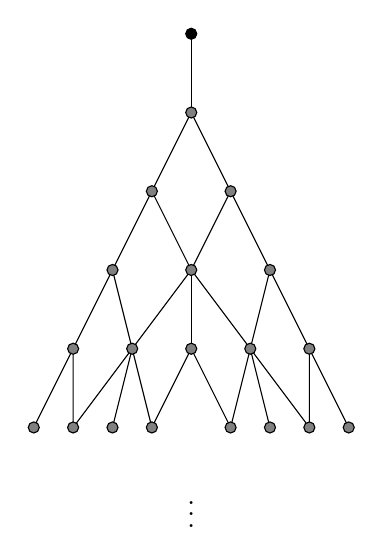
\begin{tikzpicture}[nodes={circle, draw, fill=black!50, inner sep=0pt, minimum width=4pt}]
              \draw (2,-4) -- (1.5,-3) -- (1,-2) -- (0.5,-1) -- (0,0) -- (-0.5,-1) -- (-1,-2) -- (-1.5,-3) -- (-2,-4);
        \draw (1.5,-3) -- (1.5,-4) -- (0.75,-3) -- (0,-2) -- (-0.75,-3) -- (-1.5,-4) -- (-1.5,-3);
        \draw  (1,-4) -- (0.75,-3) -- (0.5,-4) -- (0,-3) -- (-0.5,-4) -- (-0.75,-3) -- (-1,-4);
        \draw (0,-3) -- (0,-2);
        \draw (0.5,-1) -- (0,-2) -- (-0.5,-1);
        \draw (-0.75,-3) -- (-1,-2);
        \draw (0.75,-3) -- (1,-2);
        \draw (0,1) -- (0,0);
        \node[fill=black] at (0,1) {};
        \node at (0,0) {};
        \node at (-0.5,-1) {};
        \node at (0.5,-1) {};
        \node at (0,-2) {};
        \node at (1,-2) {};
        \node at (-1,-2) {};
        \node at (0,-3) {};
        \node at (0.75,-3) {};
        \node at (-0.75,-3) {};
        \node at (1.5,-3) {};
        \node at (-1.5,-3) {};
        \node at (-2,-4) {};
        \node at (-1.5,-4) {};
        \node at (-1,-4) {};
        \node at (-0.5,-4) {};
        \node at (0.5,-4) {};
        \node at (1,-4) {};
        \node at (1.5,-4) {};
        \node at (2,-4) {};
        \node[draw=none, fill=white] at (0,-5) {$\vdots$};
      \end{tikzpicture}
    \end{center}

with the root corresponding to the upper vertex of the square. 

\begin{prop}\label{grad}
Let $\mathfrak{t}$ be a bounded t-structure on $\mathscr{D}$, $\mathscr{P}$ an abelian $\mathbb{Z}$-slicing on $\heartsuit_{\mathfrak{t}}$, $\mathscr{Q}$ the associated $\mathbb{Z} \ltimes \hat{\mathbb{Z}}$-slicing on $\mathscr{D}$, $p$ a perversity. We have: 
\begin{enumerate}
\item if $\mathscr{P}$ is a perverse filtration, then $\mathscr{Q}$ satisfies the assumptions of \hyperref[pipp]{\textbf{Proposition \ref*{pipp}}} with respect to the map $\mathbb{Z} \ltimes \hat{\mathbb{Z}} \overset{f_p}{\longrightarrow} \mathbb{Z} \ltimes \hat{\mathbb{Z}}$ given by $$f_p(n,\phi)=(n+p(\lfloor \phi / 2 \rfloor),-p(\lfloor \phi / 2 \rfloor))$$ 
\item if $\mathscr{P}$ is a grading filtration, then $\mathscr{Q}$ satisfies the assumptions of \hyperref[pipp]{\textbf{Proposition \ref*{pipp}}} with respect to the map $\mathbb{Z} \ltimes \hat{\mathbb{Z}} \overset{g_p}{\longrightarrow} \mathbb{Z} \ltimes \hat{\mathbb{Z}}$ given by $$g_p(n,\phi)=(n+p(\phi),-p(\phi))$$ 
\item if $\mathscr{P}$ is a mixed filtration, then the abelian $\mathbb{Z}$-slicing induced on the heart of the bounded t-structure associated to $(g_p)_{\textnormal{\Libra}}(\mathscr{Q})$ is split 
\end{enumerate}
\end{prop}

\begin{proof}
Let's prove \textit{(2)}. Suppose $g_p(n,\phi) > g_p(m,\psi)$. Then either $m-n< p(\phi) - p(\psi)$ or both $m-n = p(\phi) - p(\psi)$ and $p(\psi) < p(\psi)$. Since by definition of t-structure we can assume $m \ge n$, the second case is absurd while in the first case, since $p$ is monotone, we have $\phi \ge \psi$ and thus by definition of perversity $$m-n<p(\phi)-p(\psi) \le \phi - \psi$$ 
and we get the desired Hom-vanishing by definition of grading filtration. \\

Suppose now $f_p(n,\phi) + 1 > f_p(m,\psi)$ and $(n+1,\phi) < (m,\psi)$. The only non absurd case is $ 1<m-n \le  p(\phi) - p(\psi)$. But then again we have $$2 \le m-n \le p(\phi)-p(\psi) \le \phi - \psi$$
and we can conclude as above. \\

To prove \textit{(1)} consider the monotone map $$\mathbb{Z} \overset{\lfloor * / 2 \rfloor}{\longrightarrow} \mathbb{Z}$$
Applying the slice functor to the latter and starting with a perverse filtration, we get a grading filtration by the properties of the floor function and the thesis follows from part \textit{(2)}. \\ 

Let's prove \textit{(3)}. We have to show that $$\mathscr{P}_{\psi}[1-p(\psi)] \subseteq \mathscr{P}_{\phi }[p(\phi)]^{\perp}$$ 
for $-p(\psi)>-p(\phi)$. We denote $n=p(\phi)-p(\psi)-1$. Assuming again $n \ge 0$, we have $n \ge 0 > p(\psi) - p(\phi) \ge \psi - \phi$ and we can then conclude by definition of mixed filtration. 
\end{proof}

Thus, in the presence of a grading (or perverse) filtration on the heart of a bounded t-structure, associating to a perversity $p$ the bounded t-structure coming from $(g_p)_{\textnormal{\Libra}}(\mathscr{Q})$ defines a morphism of $\mathbb{Z}$-posets $$\Xi^{\textnormal{op}} \longrightarrow \mathfrak{bts}(\mathscr{D})$$
we can restate this as: 

\begin{center}
\twonotes \ \textit{A grading or perverse filtration on the heart of a bounded t-structure on $\mathscr{D}$ induces a presheaf of t-structures on $\mathbb{Z} \times \mathbb{Z}$ with the product order, and thus some kind of a 'non totally ordered $\mathbb{Z} \times \mathbb{Z}$-slicing' on $\mathscr{D}$.}
\end{center}

\begin{center}
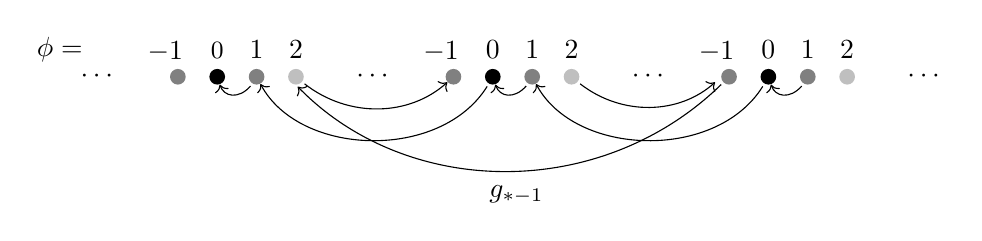
\begin{tikzpicture}

\node at (-5,0) {$\cdots$};
\draw (-4,0) node[circle,fill=gray,inner sep=2pt,label={[xshift=-4.5pt, yshift=-1pt]above: $-1$}] {};
\draw (-3.5,0) node[circle,fill,inner sep=2pt,label={[font=\small]above: $0$}] {};
\draw (-3,0) node[circle,fill=gray,inner sep=2pt,label=above: {$1$}] {} edge[->, bend left=60,looseness=1.5,shorten <=1pt,shorten >=3pt] (-3.5,0);
\draw (-2.5,0) node[circle,fill=lightgray,inner sep=2pt,label=above: {$2$}] {} edge[->, bend right=40,shorten <=1pt,shorten >=3pt] (-0.5,0);

\node at (-1.5,0) {$\cdots$};
\draw (-0.5,0) node[circle,fill=gray,inner sep=2pt,label={[xshift=-4.5pt, yshift=-1pt]above: $-1$}] {};
\draw (0,0) node[circle,fill,inner sep=2pt,label=above: {$0$}] {}  edge[->, bend left=60,shorten <=1pt,shorten >=3pt] (-3,0);
\draw (0.5,0) node[circle,fill=gray,inner sep=2pt,label=above: {$1$}] {} edge[->, bend left=60,looseness=1.5,shorten <=1pt,shorten >=3pt] (0,0);
\draw (1,0) node[circle,fill=lightgray,inner sep=2pt,label=above: {$2$}] {}  edge[->, bend right=40,shorten <=1pt,shorten >=3pt] (2.9,0);
\node at (2,0) {$\cdots$};

\draw (3,0) node[circle,fill=gray,inner sep=2pt,label={[xshift=-4.5pt, yshift=-1pt]above: $-1$}] {} edge[->, bend left=45,shorten <=1pt,shorten >=5pt] (-2.6,0);
\draw (3.5,0) node[circle,fill,inner sep=2pt,label=above: {$0$}] {} edge[->, bend left=60,shorten <=1pt,shorten >=3pt] (0.5,0);
\draw (4,0) node[circle,fill=gray,inner sep=2pt,label=above: {$1$}] {} edge[->, bend left=60,looseness=1.5,shorten <=1pt,shorten >=3pt] (3.5,0);
\draw (4.5,0) node[circle,fill=lightgray,inner sep=2pt,label=above: {$2$}] {};
\node at (5.5,0) {$\cdots$};

\node at (-5.5,0.35) {$\phi=$};
\node at (0.3,-1.5) {$g_{*-1}$};

\end{tikzpicture}
\end{center}

Now, by sending an upper set of $I \in O(\mathbb{Z})$ to its characteristic function $\chi_I$ we get an embedding $$O(\mathbb{Z})^{\textnormal{op}} \hookrightarrow \Xi$$ and the t-structure coming from $(g_{\chi_I})_{\textnormal{\Libra}}(\mathscr{Q})$ is just the tilting of $\mathfrak{t}$ with respect to the torsion pair coming from $I$. \\
The following proposition gives a characterization of the new heart obtained by the above construction. In the case of a mixed filtration, we get a splitting property which is often referred as 'decomposition theorem for perverse sheaves' in literature. \\

\begin{prop}
Let $\mathfrak{t}$ be a bounded t-structure on $\mathscr{D}$, $\mathscr{P}$ a grading filtration on $\heartsuit_{\mathfrak{t}}$, $\mathscr{Q}$ the associated $\mathbb{Z} \ltimes \hat{\mathbb{Z}}$-slicing on $\mathscr{D}$, $p$ a perversity. Denote $\mathfrak{q}$ the bounded t-structure associated to $(g_p)_{\textnormal{\Libra}}(\mathscr{Q})$. Then $\heartsuit_{\mathfrak{q}}$ consists of objects $X \in \mathscr{D}$ so that $$H_{\mathfrak{t}}^{k}(X) \in \mathscr{P}_{p^{-1}(-k)}[k]$$ 
for each $k \in \mathbb{Z}$. Moreover, if $\mathscr{P}$ is a mixed filtration then for each $X \in \heartsuit_{\mathfrak{q}}$ $$X=\bigoplus_{n \in \mathbb{Z}}H_{\mathfrak{t}}^{n}(X)$$ 
\end{prop}

\begin{proof}
This is very similar to \hyperref[tilt1]{\textbf{Proposition \ref*{tilt1}}}: we have that $X \in \heartsuit_{\mathfrak{q}}$ if and only if $$H_{\mathscr{P}}^{\phi}(H_{\mathfrak{t}}^k(X)[-k])[k]=H_{\mathscr{Q}}^{(k,\phi)}(X)=0$$ 
for $p(\phi) \not = -k$. \\
For the second part of the claim, the abelian $\mathbb{Z}$-slicing induced on $\heartsuit_{\mathfrak{q}}$ is split by \hyperref[grad]{\textbf{Proposition \ref*{grad}}} and thus by \hyperref[split]{\textbf{Proposition \ref*{split}}} $$X=\bigoplus_{(k,\phi)}H_{\mathscr{Q}}^{(k,\phi)}(X)=\bigoplus_{n \in \mathbb{Z}}H_{\mathfrak{t}}^{n}(X)$$
where the last equality comes from the first part. 
\end{proof}

\begin{exmp}
Let $$B=\bigoplus_{i\in \mathbb{N}}B_i$$ be an $\mathbb{N}$-graded ring with $B_0$ semisimple. Denote $\mathscr{A}$ the category of $\mathbb{Z}$-graded $B$-modules with only finitely many nonzero graded pieces. For $\phi \in \mathbb{Z}$, denote $\mathscr{P}_{\phi}$ the full subcategory of $\mathscr{A}$ of modules concentrated in degree $\phi$. Clearly, $\mathscr{P}$ defines an abelian $\mathbb{Z}$-slicing on $\mathscr{A}$. Following \cite{kos} we have $$\textnormal{Ext}_{\mathscr{A}}^n(\mathscr{P}_{\phi},\mathscr{P}_{\psi})=0$$
for $n>\psi - \phi$. This means that $\mathscr{P}$ is a mixed filtration and the bounded t-structure on $\mathscr{D}^b(\mathscr{A})$ associated to $(g_1)_{\textnormal{\Libra}}(\mathscr{Q})$ (where $1$ is the identity of $\mathbb{Z}$) is the 'diagonal' (or 'geometric') t-structure which appears in Koszul duality and other areas. 
\end{exmp}

\begin{exmp}
Let $M$ be an $n$-dimensional smooth complex projective variety and consider the $n$-torsion pair $\mathscr{P}$ on $\textnormal{Coh}(M)$ from \hyperref[cohh]{\textbf{Example \ref*{cohh}}}. Using Serre duality and the Grothendieck vanishing theorem, one sees that $\mathscr{P}$, seen as an abelian $\mathbb{Z}$-slicing via the inclusion $[n] \subseteq \mathbb{Z}$, is a perverse filtration. The bounded t-structure associated to $(f_p)_{\textnormal{\Libra}}(\mathscr{Q})$ is the one of perverse coherent sheaves as constructed in \cite{bez}. Following again the proof of \hyperref[t]{\textbf{Proposition \ref*{t}}}, we can use the Harder-Narasimhan filtrations from Gieseker stability to obtain an abelian $J_n$-slicing on the heart of perverse coherent sheaves as done in \cite{perpol}. 
\end{exmp}

Now we somehow review the gluing construction for t-structures in \cite{del}, but generalize it to any slicing. Our language is quite different though, and we formulate the problem very similarly to \cite{glu}. We start with two $\mathbb{Z}$-posets $J,J'$. 

\begin{defn}
Let $\mathscr{P}$ be a $J \ltimes J'$-slicing on $\mathscr{D}$. We call $\mathscr{P}$ \textbf{gluable} if it satisties the assumptions of \hyperref[pipp]{\textbf{Proposition \ref*{pipp}}} with respect to the map $J \ltimes J' \overset{e}{\longrightarrow} J' \ltimes J$ that exchanges coordinates. In this case we denote $$\overline{\mathscr{P}}=e_{\textnormal{\Libra}}(\mathscr{P})$$
\end{defn}

By a simple computation, the gluability condition reads: $\mathscr{P}_{(\phi,\psi)} \subseteq \mathscr{P}_{(\phi',\psi')}^{\perp}$ if $\psi' > \psi$ or both $\psi'+1>\psi$ and $\phi'+1 < \phi$. For example, the first condition is automatic when $\mathbb{Z}$ acts trivially on $J$ (in this case, it follows from the second one). In particular, if $\mathbb{Z}$ acts trivially on $J$, $\mathscr{P}$ is a $J$-slicing on $\mathscr{D}$ and $\mathfrak{t}_{\phi}$ is a bounded t-structure on $\mathscr{P}_{\phi}$ for each $\phi \in J$, then using \hyperref[aab]{\textbf{Proposition \ref*{aab}}} we get a $J \ltimes \mathbb{Z}$-slicing $\mathscr{Q}$ which is gluable if and only if $$\heartsuit_{\mathfrak{t}_{\psi}}[n] \subseteq \heartsuit_{\mathfrak{t}_{\phi}}^{\perp}$$
whenever both $n \le 0$ and $\phi < \psi$. 

\begin{rem}
We have a commutative diagram of $\mathbb{Z}$-posets 
\begin{center}
\begin{tikzcd}[ampersand replacement=\&]
\mathbb{Z} \ltimes \mathbb{Z} \arrow{r}{\sim} \arrow{d}{e} \& \mathbb{Z} \ltimes \hat{\mathbb{Z}} \arrow{d}{g} \\
\mathbb{Z} \ltimes \mathbb{Z} \arrow{r}{\sim}  \& \mathbb{Z} \ltimes \hat{\mathbb{Z}} 
\end{tikzcd}
\end{center}
where the horizontal isomorphism is the one from \hyperref[zet]{\textbf{Remark \ref*{zet}}}. Indeed, a $\mathbb{Z} \ltimes \mathbb{Z}$-slicing on $\mathscr{D}$ is gluable if and only if it induces a grading filtration on the heart of the associated t-structure when seen as a $\mathbb{Z} \ltimes \hat{\mathbb{Z}}$-slicing. 
\end{rem} 

An easy combinatorial calculation finally yelds the following two remarks: 
\begin{itemize}
\item  if $\mathscr{P}$ is a gluable $\hat{\mathbb{Z}} \ltimes \mathbb{Z}$-slicing on $\mathscr{D}$, then $\overline{\mathscr{P}}$ induces a grading filtration on the associated heart, allowing us again to construct new bounded t-structures depending on a perversity. 
\item if $\mathscr{P}$ is a mixed filtration on the heart of a bounded t-structure and $\mathscr{Q}$ is the associated $\mathbb{Z} \ltimes \hat{\mathbb{Z}}$-slicing on $\mathscr{D}$, then $\mathscr{Q}$ is gluable. In this case, looking at $\overline{\mathscr{Q}}$, we get a baric structure on $\mathscr{D}$ which is usually called \textbf{weight decomposition} in literature. 
\end{itemize}
In other words, the chain of implications for a $\mathbb{Z} \ltimes \hat{\mathbb{Z}}$-slicing refines to 
$$\textnormal{mixed} \implies \textnormal{gluable} \implies \textnormal{grading} \implies \textnormal{perverse} $$

%\begin{prop}
%A $J \ltimes J'$-slicing $\mathscr{P}$ on $\mathscr{D}$ is gluable if and only if it satifies the assumptions of \hyperref[pipp]{\textbf{Proposition \ref*{pipp}}} with respect to the identity (as sets) $J \ltimes J' \longrightarrow J \times J'$, where we place the product order on the right member. 
%\end{prop}
%
%\begin{proof}
 % Consider the following commutative diagram of sets
 % \begin{center}
%\begin{tikzcd}[ampersand replacement=\&]
%J \ltimes J' \arrow{r}{e} \arrow{d}{1} \& J \ltimes J' \\
%J \times J' \arrow{r}{e}  \& J \times J' \arrow{u}{1}
%\end{tikzcd}
%  \end{center}
%  The right arrow is a morphism of $\mathbb{Z}$-posets while the down one is an isomorphism of $\mathbb{Z}$-posets, and the thesis follows. 
%\end{proof}
%\begin{prop}
%Let $\mathscr{P}$ be a gluable $J \times J'$-slicing on $\mathscr{D}$. For $i = 1,2$, denote $\mathscr{P}^i=\pi_{\textnormal{\Libra}}^i(\mathscr{P})$, where $J \overset{\pi^1}{\longleftarrow} J \times J' \overset{\pi^2}{\longrightarrow} J'$ are the projections. Then for each $\psi \in J'$, $\mathscr{P}_{\psi}^2$ consists of objects $X \in \mathscr{D}$ so that $$H_{\mathscr{P}^1}^{\phi}(X) \in \mathscr{Q}_{(\phi,\psi)}$$
%for each $\phi \in J$.
%\end{prop}
%
%\begin{proof}
%We have already seen that $X \in \mathscr{P}_{\psi}^2$ if and only if $$H_{\mathscr{P}}^{\lambda}(X)=H_{\mathscr{P}}^{\lambda}(H_{\mathscr{P}^1}^{\pi^1(\lambda)}(X))=0$$
%for $\pi^2(\lambda) \not =\psi$. By fixing $\pi^1(\lambda)=\phi$ and varying $\pi^2(\lambda)$, we get the desired result. 
%\end{proof}
\newpage

\afterpage{\blankpage}
	 \section{Some applications}
\epigraph{\textit{First law of Physical Mathematics: every cloud has a silver lining.}}{Yuri Manin}
\vspace{10 mm}
\subsection{Calabi-Yau categories}

A natural condition to impose on our triangulated category is to behave just like the derived category of a variety, i.e. to posses some form of Serre duality. This is done in \cite{bon}. In particular, accordingly to our string-theoretic motivations, one can define Calabi-Yau triangulated categories as in \cite{kel}, and try to describe their slicings. \\
Suppose that $\mathscr{D}$ is $k$-linear over some field $k$ (we also assume that $\Sigma$ is $k$-linear). 

\begin{center}
\begin{figure}[h]
\begin{tikzpicture}
\node[opacity=0.7] at (6,0) {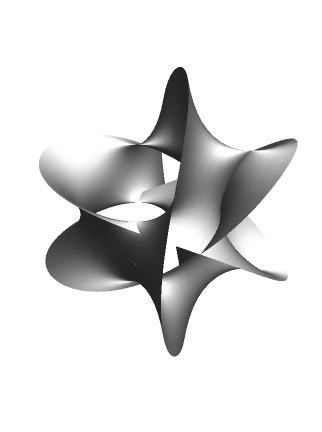
\includegraphics[width=6cm]{Sezione}};  %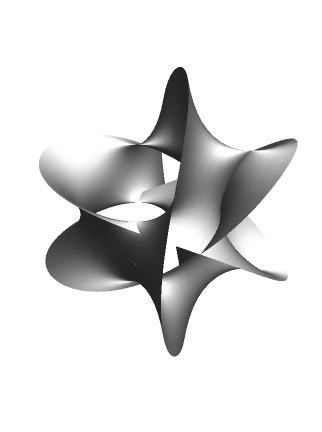
\includegraphics[scale=0.5]{Sezione}
\end{tikzpicture}
\caption{A depiction of a $3$-dimensional real projection of a complex $2$-dimensional section of the Fermat quintic in the $4$-dimensional complex projective space.}
\end{figure}
\end{center}

\begin{defn}
$\mathscr{D}$ is \textbf{Hom-finite} if for each $X,Y \in \mathscr{D}$ the graded $k$-vector space $$\textnormal{Hom}_{\mathscr{D}}^{\bullet}(X,Y)=\bigoplus_{i \in \mathbb{Z}} \textnormal{Hom}_{\mathscr{D}}(X,Y[i])$$ is finite dimensional. 
%If that's the case, we define the \textbf{Euler pairing} $$\chi(X,Y)= \sum_{i \in \mathbb{Z}} (-1)^i \textnormal{dim}_k(\textnormal{Hom}_{\mathscr{D}}(X,Y[i]))$$
\end{defn} 

Suppose moreover that $\mathscr{D}$ is Hom-finite. \\

\begin{defn}
A \textbf{Serre functor} on $\mathscr{D}$ is a $k$-linear autoequivalence $S$ so that there is a natural isomorphism of $k$-linear bifunctors from $\mathscr{D}^{\textnormal{op}} \times \mathscr{D}$ to $\textnormal{Mod}_k$: $$\textnormal{Hom}_{\mathscr{D}}(X,Y) \overset{\varphi_{X,Y}}{\longrightarrow} \textnormal{Hom}_{\mathscr{D}}(Y,S(X))^{\vee}$$
where $*^{\vee}=\textnormal{Hom}_k(*,k)$ denotes the duality functor. \\
If $n \in \mathbb{Z}$, we say that $\mathscr{D}$ is $n$-\textbf{Calabi-Yau} over $k$ if $\Sigma^n$ is a Serre functor on $\mathscr{D}$. We'll often refer to the above isomorphism as \textbf{Serre duality}.
\end{defn} 

First of all, observe that if $S$ is a Serre functor on $\mathscr{D}$, by bifunctoriality we have for each $X,Y \in \mathscr{D}$ a commutative diagram:
\begin{center}
\begin{tikzcd}[ampersand replacement=\&]
 \textnormal{Hom}_{\mathscr{D}}(X,Y)  \arrow{r}{\varphi_{X,Y}} \arrow{d}{S} \& \textnormal{Hom}_{\mathscr{D}}(Y,S(X))^{\vee}  \\ 
\textnormal{Hom}_{\mathscr{D}}(S(X),S(Y)) \arrow{r}{\varphi_{S(X),S(Y)}} \& \textnormal{Hom}_{\mathscr{D}}(S(Y),S^2(X))^{\vee} \arrow{u}{S^{\vee}}
\end{tikzcd}
\end{center}
which will legitimate us to write, as usual, equalities instead of isomorphisms. \\

\begin{exmp}
Let $A$ be a finite-dimensional algebra over $k$. Following \cite{kel}, the bounded derived category of finite dimensional $A$-modules $\mathscr{D}^b(\textnormal{Mod}_A^{\textnormal{fd}})$ has a Serre functor if and only if $A$ is of finite global dimension. In this case, the Serre functor is diven by the Nakayama functor $$\mathscr{L} A^{\vee} \otimes_A *$$ 
\end{exmp}

\begin{prop}
$\mathscr{D}$ admits a Serre functor if and only if for each $X \in \mathscr{D}$ the functor $\textnormal{Hom}_{\mathscr{D}}(X,*)^{\vee}$ from $\mathscr{D}^{\textnormal{op}}$ to $\textnormal{Mod}_k$ is representable. Moreover, the Serre functor, if it exists, is unique up to natural isomorphism of $k$-linear functors.
\end{prop}

\begin{proof}
Clearly, if $S$ if a Serre functor on $\mathscr{D}$, $S(X)$ represents $\textnormal{Hom}_{\mathscr{D}}(X,*)^{\vee}$. Conversely, for each $X \in \mathscr{D}$, choose a representative $S(X)$ for the functor $\textnormal{Hom}_{\mathscr{D}}(X,*)^{\vee}$ and a natural isomorphism of $k$-linear functors $$\textnormal{Hom}_{\mathscr{D}}(*,S(X)) \overset{\varphi_X}{\longrightarrow} \textnormal{Hom}_{\mathscr{D}}(X,*)^{\vee}$$
and this is the data that gives the desired Serre functor. \\
For the second part of the claim, if $S$ and $S'$ are Serre functors, then for each $X \in \mathscr{D}$, $S(X)$ and $S'(X)$ both represent the functor $\textnormal{Hom}_{\mathscr{D}}(X,*)^{\vee}$ and thus $S=S'$ by the Yoneda lemma. 
\end{proof}

\begin{prop}
Let $S$ be a Serre functor on $\mathscr{D}$. Then: 
\begin{enumerate}
\item $S$ commutes (up to natural isomorphism) with all the autoequivalences of $\mathscr{D}$
\item $S$ is a triangle functor 
\end{enumerate}   
\end{prop}

\begin{proof}
Pick an autoequivalence $F$ of $\mathscr{D}$. For each $X, Y \in \mathscr{D}$, using Serre duality we get: 
\begin{align*}
\textnormal{Hom}_{\mathscr{D}}(X,F(S(Y))) & =   \textnormal{Hom}_{\mathscr{D}}(F^{-1}(X),S(Y)) \\
 & =  \textnormal{Hom}_{\mathscr{D}}(Y,F^{-1}(X))^{\vee} \\
& = \textnormal{Hom}_{\mathscr{D}}(F(Y),X)^{\vee} \\
& =  \textnormal{Hom}_{\mathscr{D}}(X,S(F(Y)))
\end{align*}
Using the Yoneda lemma we conclude $FS(Y)=SF(Y)$ naturally, as desired. \\
Now we prove \textit{(2)}. First of all, using \textit{(1)}, there is an isomorphism $S \Sigma = \Sigma S$. Pick a distinguished triangle $X \overset{f}{\longrightarrow} Y \overset{g}{\longrightarrow} Z \longrightarrow $ in $\mathscr{D}$. Now, since for each $E \in \mathscr{D}$ $$\textnormal{Hom}_{\mathscr{D}}(E,*)=\textnormal{Hom}_{\mathscr{D}}(*,S(E))^{\vee}$$ 
and $\textnormal{Hom}_{\mathscr{D}}(*,S(E))^{\vee}$ is cohomological, we have that the triangle $S(X) \longrightarrow S(Y) \longrightarrow S(Z) \longrightarrow$ is special. Putting $C=\textnormal{cone}(S(f))$, we get a distinguished triangle $S(X) \longrightarrow S(Y) \longrightarrow C \overset{h}{\longrightarrow}$. By applying the Hom-functors to these two triangles and using Serre duality we get a commutative diagram with exact rows and columns: 
\begin{center}
\scalebox{0.8}{
\begin{tikzcd}[ampersand replacement=\&]
 \cdots \arrow{r} \& \textnormal{Hom}_{\mathscr{D}}(X[1],Y) \arrow{r} \arrow{d} \& \textnormal{Hom}_{\mathscr{D}}(C,S(Y)) \arrow{r} \arrow{d} \&  \textnormal{Hom}_{\mathscr{D}}(Y,Y) \arrow{r} \arrow{d} \& \cdots \\
\cdots \arrow{r} \& \textnormal{Hom}_{\mathscr{D}}(X[1],Z) \arrow{r} \arrow{d} \& \textnormal{Hom}_{\mathscr{D}}(C,S(Z)) \arrow{r}{d} \arrow{d}{\delta} \&  \textnormal{Hom}_{\mathscr{D}}(Y,Z) \arrow{r} \arrow{d} \& \cdots \\
\cdots \arrow{r} \& \textnormal{Hom}_{\mathscr{D}}(X,X) \arrow{r} \& \textnormal{Hom}_{\mathscr{D}}(C,S(X)[1]) \arrow{r} \&  \textnormal{Hom}_{\mathscr{D}}(Y,X[1]) \arrow{r}  \& \cdots \\
\end{tikzcd}
}
\end{center}
By some diagram chasing involving  \hyperref[a]{\textbf{Proposition \ref*{a}}}, we get a morphism $C \overset{a}{\longrightarrow} S(Z)$ so that $d(a)=g$ and $\delta(a)=h$. This means that the following is a morphism of special triangles: 
\begin{center}
\begin{tikzcd}[ampersand replacement=\&]
S(X) \arrow{r} \arrow{d}{1} \& S(Y) \arrow{r} \arrow{d}{1} \& C \arrow{r} \arrow{d}{a} \& S(X)[1] \arrow{d}{1} \\
S(X) \arrow{r}\& S(Y) \arrow{r}  \& S(Z) \arrow{r}  \& S(X)[1]  
\end{tikzcd}
\end{center}
Applying \hyperref[c]{\textbf{Proposition \ref*{c}}} we get $C=S(Z)$, as desired. 
\end{proof}

\begin{exmp}
If $M$ is an $n$-dimensional complex smooth projective variety, then the classical Serre duality in geometry tells us that the twist $* \otimes \omega_M[n]$ (where $\omega_M$ is the canonical bundle) is a Serre functor on $\mathscr{D}^b(\textnormal{Coh}(M))$. If $M$ is moreover a Calabi-Yau variety (i.e. the canonical bundle $\omega_M=\mathcal{O}_M$ is trivial) then we see that $\mathscr{D}^b(\textnormal{Coh}(M))$ is $n$-Calabi-Yau over $\mathbb{C}$, which is the reason of our nomenclature.  
\end{exmp}
%
%Observe that if $A \subseteq \mathscr{D}$ is a full subcategory and $S$ is a Serre functor, then $S(^{\perp}A)=A^{\perp}$. \\
%
%\begin{prop}
%Suppose that $\mathscr{D}$ has a Serre functor $S$ and that $J$ acts trivially on $\mathbb{Z}$. Let $\mathscr{P}$ be a $J$-slicing on $\mathscr{D}$. Then $\mathscr{P}_{\phi}$ is admissible and has a Serre functor for each $\phi \in J$. 
%\end{prop}
%
%\begin{proof}
%Since $\mathscr{P}_{\phi}$ is a t-structure on $\mathscr{P}_{]-\infty, \phi]}$ fixed by translation and the same holds for $\mathscr{P}_{]-\infty, \phi]}$ in $\mathscr{D}$, by ??? we can suppose $J=[2]$. Pick a t-structure $\mathfrak{t}$ on $\mathscr{D}$ fixed by translation and consider the $[2]$-slicing $\mathscr{P}=\{ \mathfrak{t}^{\perp}, \mathfrak{t} \}$. By the above observation, acting by $S$ on $\mathscr{P}$ we obtain a $[2]$-slicing $$S.\mathscr{P}=\{ S(\mathfrak{t}$$
%\end{proof}

Now, observe that we allow 'negative dimension' ($n \le 0$) in the definition of $n$-Calabi-Yau categories. Such categories exist (see \cite{hol}) and provide a counterexample to the existence of bounded t-structures, as shown below. 

\begin{prop}
Suppose that $\mathscr{D}$ is $n$-Calabi-Yau with $n<0$. Then any t-structure on $\mathscr{D}$ is fixed by translation. In particular, $\mathfrak{bts}(\mathscr{D})=\emptyset$. 
\end{prop}

\begin{proof}
Let $\mathfrak{t}$ be a t-structure on $\mathscr{D}$. For each $X \in \heartsuit_{\mathfrak{t}}$, using Serre duality  $$\textnormal{End}_{\mathscr{D}}(X)=\textnormal{Hom}_{\mathscr{D}}(X[-n],X)^{\vee}$$
Since $n<0$, the latter is zero and thus $X=0$. By arbitrariness of $X$, $\heartsuit_{\mathfrak{t}}=0$, as desired. \\
The second claim follows from the fact that if a t-structure is fixed by translation then it has zero heart, and thus can't be bounded. 
\end{proof}

\begin{prop}\label{tta}
Suppose that $\mathscr{D}$ is $n$-Calabi-Yau. Suppose moreover that one of the following conditions holds: 
\begin{enumerate} 
\item $n \le 1$ 
\item the action of $\mathbb{Z}$ on $J$ is trivial 
\end{enumerate}  
Then any $J$-slicing on $\mathscr{D}$ is hereditary. 
\end{prop}

\begin{proof}
Pick $X \in \mathscr{P}_{\phi}$, $Y \in \mathscr{P}_{\psi}$ and suppose $\phi + 1 < \psi$ in $J$. Then using Serre duality we get $$\textnormal{Hom}_{\mathscr{D}}(X,Y)=\textnormal{Hom}_{\mathscr{D}}(Y,X[n])^{\vee}$$
Now, $X[n]$ is semistable of phase $\phi + n $ with respect to $\mathscr{P}$. If condition \textit{(1)} holds, then $\phi + n \le \phi + 1 < \psi$. It condition \textit{(2)} holds, then $\phi + n = \phi < \psi$. In either case, the latter is zero, as desired. 
\end{proof}

\begin{prop}\label{ttb}
Let $M$ be an $n$-dimensional Calabi-Yau variety and suppose that the action of $\mathbb{Z}$ on $J$ is trivial. Then any $J$-slicing on $\mathscr{D}^b(\textnormal{Coh}(M))$ is trivial\footnote{A $J$-slicing $\mathscr{P}$ on $\mathscr{D}$ is called trivial if $\mathscr{P}_{\phi}=\mathscr{D}$ for some $\phi \in J$.}.
\end{prop}

\begin{proof}
Denote $\mathscr{D}=\mathscr{D}^b(\textnormal{Coh}(M))$ and let $\mathscr{P}$ be a $J$-slicing on $\mathscr{D}$. Now the structure sheaf $\omega_M=\mathcal{O}_M$ and the skyscraper sheaves of points $\mathcal{O}_x$ (with $x \in M$) are indecomposable in $\textnormal{Coh}(M)$ and, since the latter is closed under direct summands in $\mathscr{D}$ by \hyperref[ttc]{\textbf{Proposition \ref*{ttc}}}, they are indecomposable in $\mathscr{D}$ as well. But then they are semistable with respect to $\mathscr{P}$ by \hyperref[tta]{\textbf{Proposition \ref*{tta}}}. Now, using Serre duality, for each $x \in M$ $$\textnormal{Hom}_{\mathscr{D}}(\mathcal{O}_x,\mathcal{O}_M[1])=\textnormal{Hom}_{\mathscr{D}}(\mathcal{O}_M,\mathcal{O}_x)^{\vee} \not = 0 $$
and thus all those sheaves must have the same phase $\phi$. This means that if $\psi \not = \phi$, then the subcategory $\mathscr{P}_{\psi}$ is orthogonal (either on right or left) to all the skyscraper sheaves and their translations, and thus $\mathscr{P}_{\psi}=0$. In other words, $\mathscr{P}_{\phi}=\mathscr{D}$, as desired.  
\end{proof}

\begin{prop}\label{tte}
Let $M$ be an $n$-dimensional Calabi-Yau variety. If there is a nontrivial $J$-slicing on $\mathscr{D}^b(\textnormal{Coh}(M))$ then $J=\mathbb{Z} \ltimes I$ for some totally ordered set $I$.
\end{prop}

\begin{proof}
If $\mathscr{P}$ is a nontrivial $J$-slicing, applying the slice functor to the morphism $J \longrightarrow I(J)$ we get a trivial $I(J)$-slicing by \hyperref[ttb]{\textbf{Proposition \ref*{ttb}}} and we conclude using \hyperref[ttd]{\textbf{Proposition \ref*{ttd}}}.
\end{proof}

Now we deal with elliptic curves (i.e. Calabi-Yau varieties of dimension $1$). All the algebro-geometric facts stated below are taken from \cite{ati}. Let $M$ be a complex elliptic curve and denote $\mathscr{D}=\mathscr{D}^b(\textnormal{Coh}(M))$. Denote moreover $\overline{\mathbb{Q}}=\mathbb{Q} \sqcup \{ \infty \}$ with the usual order. If $q=\frac{a}{b} \in \overline{\mathbb{Q}}=\mathbb{Q} \sqcup \{ \infty \}$ with $a \not = 0$ and $b>0$ (or $a=0$, $b=1$, or $a=1$, $b=0$) then we define $E_q$ as the set of indecomposable coherent sheaves on $M$ of degree $a$ and rank $b$. If $X \not = Y \in E_q$ then $$\textnormal{Hom}_{\mathscr{D}}(X,Y)=\textnormal{Hom}_{\mathscr{D}}(Y,X)=0$$
and if $p>q$ then for each $X \in E_p$, $Y \in E_q$ $$\textnormal{Hom}_{\mathscr{D}}(X,Y)=0 \not = \textnormal{Hom}_{\mathscr{D}}(Y,X)=\textnormal{Hom}_{\mathscr{D}}(X,Y[1])^{\vee}$$ We denote the set of all indecomposable coherent sheaves on $M$ by $$E=\coprod_{q \in \overline{\mathbb{Q}}} E_q$$ 
Now, $\textnormal{Coh}(M)$ is a Krull-Schmidt category, and thus every coherent sheaf is direct sum of indecomposable ones. This means that if we choose a total order on each set $E_q$ in an arbitrary way and take the lexicographical coproduct order on $E$, then $$\mathscr{M}_X^0= \langle X \rangle $$ 
with $X \in E$ defines an abelian $E$-slicing $\mathscr{M}^0$ on $\textnormal{Coh}(M)$ which by \hyperref[v]{\textbf{Proposition \ref*{v}}} induces a $\mathbb{Z} \ltimes E$-slicing $\mathscr{M}$ on $\mathscr{D}$. We call $\mathscr{M}$ the \textbf{Mumford-Takemoto} slicing (beware that it depends on the choices made for $E$). The name comes from the fact that applying the slice functor to the projection $$E \longrightarrow \overline{\mathbb{Q}}$$ one obtains Mumford stability from the introduction. We now show that the Mumford-Takemoto slicing is indeed the 'finest' one. 

\begin{prop}
Let $\mathscr{P}$ be a nontrivial $J$-slicing on $\mathscr{D}$. Then there is a choice for $E$ and a morphism of $\mathbb{Z}$-posets $\mathbb{Z} \ltimes E \overset{f}{\longrightarrow} J$ so that $$\mathscr{P}=f_{\textnormal{\Libra}}(\mathscr{M})$$
\end{prop}

\begin{proof}
Pick $q \in \overline{\mathbb{Q}}$. Each $X \in E_q$ is indecomposable and thus, by \hyperref[tta]{\textbf{Proposition \ref*{tta}}} ($n=1$), is semistable with respect to $\mathscr{P}$ of some phase $f(E_q) \in J$. Pulling back the ordering on $J$  we get a partial order on $E_q$, and thus an order on the whole $E$. We can extend the latter to a total order using the Zorn's lemma. By the hom-vanishing properties above we have a morphism of posets $E \overset{f}{\longrightarrow} J$ which extends to a morphism of $\mathbb{Z}$-posets $\mathbb{Z} \ltimes E \overset{f}{\longrightarrow} J$. By definition, for each $\phi \in J$ we have $(f_{\textnormal{\Libra}}(\mathscr{M}))_{\phi} \subseteq \mathscr{P}_{\phi}$ and we conclude using \hyperref[fat]{\textbf{Proposition \ref*{fat}}}.
\end{proof}

In particular, using \hyperref[u]{\textbf{Proposition \ref*{u}}} we get all the bounded t-structures on $\mathscr{D}$, which are all, up to translation, tiltings (with respect to some split torsion pairs) of the standard one and have hearts with bounded derived category equivalent to $\mathscr{D}$ by \hyperref[equiv]{\textbf{Remark \ref*{equiv}}}!  

\newpage
\subsection{Exceptional collections}
In this section, we give a way to build up semiorthogonal decompositions and t-structures with finite length hearts from a very simple set of data. The main reference is \cite{hel}. \\ 
Now, let $k$ be a field and suppose that $\mathscr{D}$ is $k$-linear and Hom-finite. Denote $\mathscr{D}(k)=\mathscr{D}^b(\textnormal{Mod}_k^{\textnormal{fin}})$ the bounded derived category of finite-dimensional $k$-vector spaces. First of all, by \hyperref[trala]{\textbf{Example \ref*{trala}}} $\mathscr{D}(k)$ is equivalent to the category of finite-dimensional $\mathbb{Z}$-graded $k$-vector spaces, and we'll implicitly use this identification for the rest of the section. \\
Now, we have a bifunctor $\mathscr{D}(k) \times \mathscr{D} \longrightarrow \mathscr{D}$ which sends $V=\oplus_{i \in \mathbb{Z}}V_i$ and $X \in \mathscr{D}$ to $$V \otimes X=\bigoplus_{i \in \mathbb{Z}} X[-i]^{\oplus \textnormal{dim}_k(V_i)}$$ 
Moreover, we have by an easy check an isomorphism of functors $$\textnormal{Hom}_{\mathscr{D}}^{\bullet}(Y,V \otimes X)=V \otimes \textnormal{Hom}_{\mathscr{D}}^{\bullet}(Y,X)$$
where the second tensor product is the one in the category of graded vector spaces. Thus, for $X,Y \in \mathscr{D}$ we have 
\begin{align*}
\textnormal{End}_{\mathscr{D}(k)}(\textnormal{Hom}_{\mathscr{D}}^{\bullet}(X,Y)) & = \textnormal{Hom}_{\mathscr{D}}^{\bullet}(X,Y)^{\vee} \otimes \textnormal{Hom}_{\mathscr{D}}^{\bullet}(X,Y)  \\
&=\textnormal{Hom}_{\mathscr{D}}^{\bullet}(X,\textnormal{Hom}_{\mathscr{D}}^{\bullet}(X,Y)^{\vee} \otimes Y) \\
&=\textnormal{Hom}_{\mathscr{D}}^{\bullet}(\textnormal{Hom}_{\mathscr{D}}^{\bullet}(X,Y)\otimes X,Y)
\end{align*}
The identity in the first member induces morphisms in $\mathscr{D}$: 
$$X \longrightarrow \textnormal{Hom}_{\mathscr{D}}^{\bullet}(X,Y)^{\vee} \otimes Y$$
$$\textnormal{Hom}_{\mathscr{D}}^{\bullet}(X,Y) \otimes X[-1] \longrightarrow Y[-1]$$
We denote $R_YX$ (resp. $L_XY$) the cone of the first (resp. second) morphism and call it the \textbf{right} (resp. \textbf{left}) \textbf{mutation} of $X$ induced by $Y$ (resp. of $Y$ induced by $X$). \\

\begin{defn} 
An object $E \in \mathscr{D}$ is called \textbf{exceptional} if the functor $* \otimes E$ is fully faithful, or, in other words, if $$\textnormal{dim}_k\textnormal{Hom}_{\mathscr{D}}(E,E[i])=\begin{cases} 1 & i=0 \\ 0 & \textnormal{otherwise} \end{cases}$$ An \textbf{exceptional collection} is a finite sequence of exceptional objects $\{ E_0, \cdots , E_n \}$ so that $$\textnormal{Hom}^{\bullet}_{\mathscr{D}}(E_i,E_j)=0 \  for \ i>j$$
We call an exceptional collection 
\begin{itemize}
\item \textbf{full} if $\mathscr{D}$ is the thick subcategory generated by the collection
\item \textbf{ext} if $\textnormal{Hom}_{\mathscr{D}}(E_i,E_j[n])=0$ for $i<j$ and $n \le 0$
%\item \textbf{strong} if $\textnormal{Hom}_{\mathscr{D}}(E_i,E_j[n])=0$ for $i < j$ and $n \not = 0$
\end{itemize}
\end{defn}

If $E$ is an exceptional object, then by \hyperref[d]{\textbf{Proposition \ref*{d}}} $\langle E \rangle$ consists of direct sums of copies of $E$ and is equivalent to the category of finite dimensional $k$-vector spaces.  \\

\begin{prop}\label{mim}
Let $\mathfrak{e}=\{  E_0, \cdots , E_n \}$ an exceptional collection on $\mathscr{D}$. Then:
\begin{enumerate}
\item $\mathscr{R}^{\mathfrak{e}}=\{ \langle \langle E_0 \rangle \rangle , \cdots , \langle \langle E_n \rangle \rangle, ^{\perp}\langle \langle \mathfrak{e} \rangle \rangle \}$ is an $[n+1]$-slicing on $\mathscr{D}$ with $$\tau_{\mathscr{R}^{\mathfrak{e}}}^{\ge i}(X)=R_{E_i}R_{E_{i-1}} \cdots R_{E_0}X[i]$$
\item  $\mathscr{L}^{\mathfrak{e}}=\{ \langle \langle E_0 \rangle \rangle , \cdots , \langle \langle E_n \rangle \rangle, \langle \langle \mathfrak{e} \rangle \rangle ^{\perp}\}$ is an $[n+1]^{\textnormal{op}}$-slicing on $\mathscr{D}^{\textnormal{op}}$ with $$\tau_{\mathscr{L}^{\mathfrak{e}}}^{\ge i}(X)=L_{E_i}L_{E_{i+1}} \cdots L_{E_n}X$$
\end{enumerate}
%For $0 \le i \le n$ denote $\mathscr{P}_i$ the thick subcategory generated by $E_i$ (or, in other words, the full subcategory of direct sums of translations of $E_i$). Then $\mathscr{P}$ is a $[n]$-slicing on $\mathscr{D}$ with equivalences $\mathscr{P}_i=\mathscr{D}(k)$.
\end{prop}

\begin{proof}
We'll just show \textit{(1)}, the other claim is proved similarly. Pick $0 \not = X \in \mathscr{D}$ and denote $$X_i=R_{E_{n-i}}R_{E_{n-i-1}} \cdots R_{E_0}X[i]$$ (we set $X_{n+1}=X$). Then by definition we have a distinguished triangle for each $0 \le i \le n$ $$X_i \longrightarrow X_{i+1} \longrightarrow \textnormal{Hom}_{\mathscr{D}}^{\bullet}(X_{i+1},E_{n-i})^{\vee} \otimes E_{n-i}[i+1] \longrightarrow$$ 
Applying the cohomological functor $\textnormal{Hom}_{\mathscr{D}}^{\bullet}(*,E_{n-i})$ to the above triangle we see that $\textnormal{Hom}_{\mathscr{D}}^{\bullet}(X_i,E_{n-i})=0$. But then, applying $\textnormal{Hom}_{\mathscr{D}}^{\bullet}(*,E_j)$ with $j<n-i$ we see inductively that $\textnormal{Hom}_{\mathscr{D}}^{\bullet}(X_i,E_j)=0$. In particular, $\textnormal{Hom}_{\mathscr{D}}^{\bullet}(X_0,E_i)=0$ for all $i$ which means $X_0 \in ^{\perp}\langle \langle \mathfrak{e} \rangle \rangle$, and this concludes the construction of the desired Postnikov tower. 
\end{proof}

\begin{prop}
Let $\mathfrak{e}=\{  E_0, \cdots , E_n \}$ a full exceptional collection on $\mathscr{D}$. Then $$K_0(\mathscr{D})=\mathbb{Z}^{n+1}$$ 
with $\mathfrak{e}$ as generators. In particular, all full exceptional collections have the same length. 
\end{prop}

\begin{proof}
We have $K_0(\textnormal{Mod}_k^{\textnormal{fin}})=K_0(\mathscr{D}(k))=\mathbb{Z}$ and using \hyperref[mam]{\textbf{Proposition \ref*{mam}}} on the semiorthogonal decomposition $\mathscr{R}^{\mathfrak{e}}$ we get the result. 
\end{proof}

If $\mathfrak{e}=\{  E_0, \cdots , E_n \}$ is an exceptional collection, considering the standard t-structure on $\mathscr{D}(k)$ and applying \hyperref[aab]{\textbf{Proposition \ref*{aab}}} we see that $$\mathscr{Q}_{(i,k)}=\langle E_i[k] \rangle $$ $$\mathscr{Q}_{\infty}=^{\perp}\langle \langle \mathfrak{e} \rangle \rangle$$ defines a $([n] \ltimes \mathbb{Z}) \sqcup \{ \infty \}$-slicing $\mathscr{Q}$ on $\mathscr{D}$ (we make $\mathbb{Z}$ fix $\infty$). The component at $\infty$ (i.e. $^{\perp}\langle \langle \mathfrak{e} \rangle \rangle$) is called \textbf{Kuznetsov component} and is an important invanriant for triangulated categories possessing an exceptional collection. Clearly, the collection is full if and only if the Kuznetsov component vanishes, and in this case $\mathscr{Q}$ is just a $[n] \ltimes \mathbb{Z}$-slicing. Moreover, the collection is full and ext if and only if $\mathscr{Q}$ is gluable, and considering $\overline{\mathscr{Q}}$ we obtain a bounded t-structure whose heart is $\langle \mathfrak{e} \rangle$. \\

\begin{exmp}
Consider a smooth hypersurface $M$ in $\mathbb{CP}^{n+1}$ of degree $d \le n+2$. Then $\mathscr{D}^b(\textnormal{Coh}(M))$ has an exceptional collection of length $n+1-d$, which is the pullback of the one from \hyperref[kuzz]{\textbf{Example \ref*{kuzz}}}. If $d$ divides $n+2$, then the associated Kuznetsov component is a Calabi-Yau triangulated category of dimension $(n+2)(d-2)/d$, as shown in \cite{kuzz} and thus can be thought as a categorification of the Jacobian variety. Indeed, one can prove Torelli-type theorems in this context: for cubic fourfolds, see \cite{macc}. 
\end{exmp}

\begin{prop}\label{mom}
Let $\mathfrak{e}=\{ E_0, \cdots , E_n \}$ be a full ext exceptional collection on $\mathscr{D}$. Then $\langle \mathfrak{e} \rangle$ is an abelian category of finite length (i.e. both artinian and noetherian) whose simple objects (up to isomorphism) are $E_0, \cdots , E_n$. \\
\end{prop}

\begin{proof}
First of all, $\langle \mathfrak{e} \rangle$ is abelian since it is the heart of a t-structure. Since we obtained $\langle \mathfrak{e} \rangle$ from a $\mathbb{Z} \ltimes [n]$-slicing, we have that $\{ \langle E_0 \rangle , \cdots , \langle E_n \rangle \}$ is an $n$-torsion pair on $\langle \mathfrak{e} \rangle$. Pick $0 \not = X \in \langle \mathfrak{e} \rangle$ and consider its Harder-Narasimhan filtration $$0=X_0 \subseteq \cdots \subseteq X_m=X$$ 
Now for each $i$, $X_i / X_{i-1} = E_{k_i}^{\oplus t_i}$ for some $k_i$, $t_i$. If $t_i > 1$, then there is an $X_{i-1} \subseteq Y \subseteq X_i$ so that $Y / X_{i-1}=E_{k_i}$ and $X_i / Y = E_{k_i}^{t_i-1}$. Iterating this argument, we get a filtration of $X$ whose factors are all in $\mathfrak{e}$. If we show that the $E_i$'s are simple, this is the desired Jordan-H{\"o}lder filtration. Let's show that the objects in $\mathfrak{e}$ are simple. Pick a subobject $0 \not = A \subseteq E_i$. By looking at the first step of the Harder-Narasimhan filtration, there is a $j$ and an inclusion $E_j \subseteq A$. But by definition of ext exceptional collection, we have $i=j$ and thus $A=E_i$, as desired. Since we have already constructed Jordan-H{\"o}lder filtrations, we get the the finite-length property. 
\end{proof}

\begin{exmp}\label{kuzz}
By \hyperref[mim]{\textbf{Proposition \ref*{mim}}} and \hyperref[ttb]{\textbf{Proposition \ref*{ttb}}} we see that Calabi-Yau varieties cannot have full exceptional collections on the bounded derived category of their coherent sheaves. However, using the Euler exact sequences, one sees that $$\{ \mathcal{O}_{\mathbb{CP}^n}, \mathcal{O}_{\mathbb{CP}^n}(1)[-1], \cdots, \mathcal{O}_{\mathbb{CP}^n}(n)[-n] \}$$ is an ext full exceptional collection on $\mathscr{D}^b(\textnormal{Coh}(\mathbb{CP}^n))$ (see \cite{hel}). In this case, the abelian category obtained from \hyperref[mom]{\textbf{Proposition \ref*{mom}}} is equivalent to the bounded derived category of finite-dimensional modules over the complex path algebra of the quiver 
\begin{center}
\begin{tikzcd}[ampersand replacement=\&]
\bullet  \arrow[bend left=50]{r}{\alpha_0^0}[swap]{\vdots} \arrow[bend right=50]{r}[swap]{\alpha_0^n} \& \bullet \& \cdots \& \bullet  \arrow[bend left=50]{r}{\alpha_{n-1}^0}[swap]{\vdots} \arrow[bend right=50]{r}[swap]{\alpha_{n-1}^n} \& \bullet
\end{tikzcd}
\end{center}
with relations $\alpha_{i+1}^j \alpha_i^k=\alpha_{i+1}^k\alpha_i^j$.
\end{exmp}

Thus, for example, if $\mathfrak{e}$ is a full ext exceptional collection, one can choose $n+1$ elements in $\mathbb{H}$ and apply the machine of \hyperref[brie]{\textbf{Example \ref*{brie}}} to construct $\mathbb{R}$-slicings on $\mathscr{D}$. This is what is done in \cite{mac} in the case of $\mathscr{D}^b(\textnormal{Coh}(\mathbb{CP}^1))$ with the exceptional collection from the above example.

%\begin{defn}
%Let $\mathfrak{e}=\{E_0, \cdots , E_n \}$ be an exceptional collection on $\mathscr{D}$, $0 \le i < n$. The $i$-\textbf{th right mutation} of that exceptional collection is the exceptional collection $$R_i(\mathfrak{e})=\{  E_0, \cdots, E_{i-1}, E_{i+1}, R_{E_{i+1}}E_i,E_{i+2}, \cdots,E_n \}$$
%\end{defn}
%
%Recall that the braid group $B_{n+1}$ is defined as the free group on generators $\sigma_0, \cdots, \sigma_{n-1}$ with relations 
%\begin{align*}
%\sigma_i \sigma_j&=\sigma_j \sigma_i \ &for \ | i-j | >1 \\
%\sigma_i \sigma_{i+1} \sigma_i&=\sigma_{i+1} \sigma_i \sigma_{i+1} \ &for \ 0 \le i < n-1
%\end{align*}
%
%\begin{prop}
%The braid group $B_{n+1}$ acts on the set of exceptional collections on $\mathscr{D}$. This action preserves fullness. 
%\end{prop}
%
%\begin{proof}
%We define the action on the generators as $$\sigma_i.\mathfrak{e}=R_i(\mathfrak{e})$$
%and we have to check that it is well-defined. Clearly, the first relation of the braid group is satistied. For the second relation, it suffices to show that for an exceptional collection $\{ E_0, E_1, E_2 \}$ we have $$R_{R_{E_2}E_1}R_{E_2}E_0=R_{E_2}R_{E_1}E_0$$
%By definition we have a distinguished triangle $$E_0 \longrightarrow \textnormal{Hom}_{\mathscr{D}}^{\bullet}(E_0,E_1)^{\vee} \otimes E_1 \longrightarrow R_{E_1}E_0 \longrightarrow $$ 
%Now, since $\textnormal{Hom}_{\mathscr{D}}^{\bullet}(E_0,E_1)=\textnormal{Hom}_{\mathscr{D}}^{\bullet}(R_{E_2}E_0,R_{E_2}E_1)$, applying the triangle functor $R_{E_2}*$ to the above triangle we get distinguished triangle: 
%\begin{center}
%
%\scalebox{0.9}{
%$R_{E_2}E_0 \longrightarrow \textnormal{Hom}_{\mathscr{D}}^{\bullet}(R_{E_2}E_0,R_{E_2}E_1)^{\vee} \otimes R_{E_2}E_1 \longrightarrow R_{E_2}R_{E_1}E_0 \longrightarrow $
%}
%\end{center}
%which is what we wanted. 
%\end{proof}
%
%FALLO COI SINISTRII!!! O FORSE NO STICAZZ\\
%Now, $B_{n+1}$ contains the following distinguished element: 
%$$\delta=(\sigma_0 \cdots \sigma_{n-1}) \cdots (\sigma_0 \sigma_1) \sigma_0$$
%which satisfies $\delta^{-1} \sigma_i \delta = \sigma_{n-i}$ for all $i$. If $\mathfrak{e}$ is an exceptional collection, we call $\delta.\mathfrak{e}$ the \textbf{dual collection}. Explicitly, $$\delta.\mathfrak{e}=\{E_n, R_{E_n}E_{n-1}, \cdots , R_{E_n} \cdots R_{E_1}E_0 \}  $$\\
%
%\begin{prop}
%Let $\mathfrak{e}=\{E_0, \cdots , E_n \}$ be a full strong exceptional collection and denote $\delta.\mathfrak{e}=\{F_0, \cdots , F_n \}$. Then 
%\end{prop}

\begin{exmp}
This is vague and in part conjectural. Fix a field $k$ and denote $\mathscr{D}\textnormal{TM}_k$ the triangulated category of mixed Tate $\mathbb{Q}$-motives over $k$. Following \cite{lev}, the Tate objects $\{ \mathbb{Q}(n) \}_{n \in \mathbb{Z}}$ form an 'infinite full exceptional collection': this means that $$\mathscr{P}_{\phi}=\langle \langle \mathbb{Q}(\phi) \rangle \rangle $$ 
with $\phi \in \mathbb{Z}$ defines a baric structure (i.e. a $\hat{\mathbb{Z}}$-slicing) with equivalences $\mathscr{P}_{\phi} = \mathscr{D}(\mathbb{Q})$, and thus a $\hat{\mathbb{Z}} \ltimes \mathbb{Z}$-slicing $\mathscr{Q}$ on $\mathscr{D}\textnormal{TM}_k$. The collection being ext (i.e. $\mathscr{Q}$ being gluable) means that $$0=\textnormal{Hom}_{\mathscr{D}\textnormal{TM}_k}(\mathbb{Q}(i),\mathbb{Q}(j)[n])=K_{2(j-i)-n}(k)^{(j-i)}$$
for $i<j$ and $n \le 0$, where $K_a(k)$ is the $a$-th higher $K$-theory group of the point $\textnormal{Spec}(k)$ and $K_a(k)^{(b)}$ is the weight $b$ summand of $K_a(k) \otimes_{\mathbb{Z}} \mathbb{Q}$ with respect to the Adams action (in other words, $K_a(k)^{(b)}$ is the $a$-th $b$-codimensional Bloch's higher Chow group of $\textnormal{Spec}(k)$ with rational coefficients). \\
This means that $\mathscr{Q}$ is gluable if and only if the Beilinson-Soul\'e conjecture holds over $k$ and the t-structure coming from $\overline{\mathscr{Q}}$ is the conjectural motivic t-structure of Tate motives. Since in this case we get a grading filtration on the heart of the latter, using \hyperref[grad]{\textbf{Proposition \ref*{grad}}} one can also define 'perverse motivic' t-structures depending on a perversity, as done in \cite{soer2}. \\
Moreover, if $k$ is a number field, a celebrated computation due to Borel shows that not only the latter conjecture holds over $k$ but the t-structure of Tate motives (whose heart we denote $\textnormal{TM}_k$) is hereditary and hence, by  \hyperref[equiv]{\textbf{Remark \ref*{equiv}}}, there is a triangulated equivalence $$\mathscr{D}^b(\textnormal{TM}_k)=\mathscr{D}\textnormal{TM}_k$$
This result, conjectured in \cite{lev}, appears with a different proof in \cite{wild}. 
\end{exmp}


\afterpage{\blankpage}
\clearpage 
\bibliographystyle{alpha}
\bibliography{tesi}
\end{document}
